\chapter{Декларативная Вычислительная Модель}

\epigraph{``Non sunt multiplicanda entia praeter necessitatem.'' \\ \emph{``Не следует множить сущее без необходимости.''}}{--- Бритва Оккама, \emph{Уильям Оккам (1285-1349?)}}

Программирование состоит из трёх частей:

\begin{itemize}
\item{Первое --- \emph{модель вычисления} --- формальная система, определяющая язык и то, как исполняются конструкции языка (например, выражения и определения) в абстрактной машине. В контексте этой книге нам интересны модели вычислений, полезные и интуитивные для программистов. Смысл этого абзаца станет более ясным позже, когда мы определим одну из моделей вычислений.}

\item{Второе, набор техник программирования и принципы архитектуры программ, создаваемых в языке вычислительной модели. Иногда мы будем называть это \emph{моделью программирования (programming model)}. Модель программирования всегда строится на основе вычислительной модели.}

\item{Третье, набор техник рассуждения, позволяющих выводить умозаключения о программах, что в свою очередь, позволит укрепить уверенность в том, что эти программы ведут себя корректно и подсчитать эффективность программ.}
\end{itemize}

Вышеприведённое определение вычислительной модели является очень общим. Не все вычислительные модели, определённые подобным образом будут полезны для программистов. Что такое разумная вычислительная модель? Интуитивно мы можем сказать, что разумная вычислительная модель --- это модель, отвечающая нескольким параметрам:

\begin{enumerate}
\item{модель может быть использована для решения большинства проблем,}
\item{модель обладает прямолинейными и практичными техниками рассуждения и}
\item{модель, которую можно эффективно реализовать.}
\end{enumerate}

Позже мы вернёмся к этому вопросу и поговорим о нём поподробнее. Первой и самой простой вычислительной моделью, которую мы будем изучать, является \emph{декларативное программирование (declarative programming)}. Сейчас мы определим декларативное программирование как вычисление функций через частичные структуры данных. Иногда такой подход называют программированием \emph{без состояний (stateless)}, в противоположность программированию с \emph{состояниями (stateful)} (также называемому как \emph{императивное} программирование), рассматриваемому в Главе 6.

Декларативная модель, упоминаемая в этой главе, --- это одна из наиболее фундаментальных моделей вычисления. Она включает в себя идею, лежащую в основе двух главных декларативных парадигм, а именно, функциональное и логическое программирование. Декларативная модель включает в себя программирование с использованием функций поверх завершённых значений, как в Scheme и Standard ML. Также, она включает в себя детерминированную логику программирования, как в Prolog при программировании без поиска. И наконец, декларативная модель может использоваться при параллельном программировании без потери положительных сторон (смотрите Главу 4).

Декларативное программирование --- это большая область, большинство идей в более выразительных вычислительных моделях уже находятся здесь, хотя бы в зачаточной форме. Поэтому декларативное программирование представлено в двух главах. Эта глава определяет вычислительную модель и практические языки, основанные на ней. Следующая глава, Глава 3, служит в качестве введения в техники программирования этого языка. Последующие главы расширяют базовую модель дополнительными концепциями. Некоторые наиболее важные --- это обработка исключений, параллелизм, компоненты (для больших программ), возможности (инкапсуляции и безопасности) и состояние (введение в объекты и классы). В контексте параллелизма, мы будем разговаривать о работе с данными, о ленивых программах, о передаче сообщений, об активных объектах, о мониторах и транзакциях. Также мы поговорим об архитектуре пользовательского интерфейса, о дистирбуции (включая отказоустойчивость) и ограничениях (включая поиск).

\subsection*{Структура главы}

Эта глава состоит из семи разделов:

\begin{itemize}
\item{В Разделе 2.1 рассматривается определение синтаксиса и семантики практических языков программирования. Синтаксис определяется через контекстно-независимое грамматическое расширение с языковыми ограничениями. Семантика определена в двух шагах: транслированием практического языка в простой язык ядра с последующей подачей семантики языка ядра. Эти техники будут использоваться на протяжении всей книги. Эта глава использует их для определения декларативной модели вычисления.}

\item{Следующие три раздела определяют синтаксис и семантику декларативной модели:

  \begin{itemize}
\item{В Разделе 2.2 рассматриваются структуры данных: единое присваиваемое хранилище и его содержимое, частичные значения и переменные, хранящие поток данных.}

\item{В Разделе 2.3 рассматривается определение синтаксиса языка ядра.}

\item{В Разделе 2.4 рассматривается семантика языка ядра в терминах простой абстрактной машины. Семантики спроектированы так, чтобы быть интуитивными и давать возможность непосредственного рассуждения о корректности и сложности.}
  \end{itemize}
}

\item{В Разделе 2.5 определён практичный язык программирования на базе языка ядра.}

\item{В Разделе 2.6 декларативная модель расширяется \emph{обработкой исключений (exception handling)}, позволяющей программам обрабатывать непредсказуемые и исключительные ситуации.}

\item{В Разделе 2.7 тема декларативной модели расширена, что позволит заинтересованным читателям углубить знания этой модели.}
\end{itemize}

\section{Определение практичных языков программирования}

Языки программирования гораздо проще чем естественные языки, но, всё же они могут обладать удивительно богатым синтаксисом, наборами абстракций и библиотек. Это особенно справедливо в отношении языков, используемых для решения задач из реального мира, эти языки мы будем называть \emph{практичными (practical)} языками. Практичный язык подобен ящику с инструментами опытного механика: много инструментов для различных целей и все инструменты используются по своим назначениям.

В этом разделе раскрываются понятия, используемые на протяжении всей книги: то, как мы представляем синтаксис (``грамматику'') и семантику (``значение'') практичного языка программирования. С этой базой мы готовы перейти к первой вычислительной модели в этой книге, а именно --- модель декларативного вычисления. Мы будем продолжать использовать эти техники на протяжении всей книги для определения вычислительных моделей.

\subsection{Синтаксис языка}

Синтаксис языка определяет \emph{корректность (legal)} программ, то есть, программы, которые можно удачно запустить на исполнение. Но что именно делает запущенная программа нас, в данный момент, не волнует. Это семантика и она будет рассматриваться в следующем разделе.

\subsubsection{Грамматика}

Грамматика --- это набор правил, определяющих конструирование 'предложений' из 'слов'. Грамматика может использоваться как для естественных языков, таких как Английский или Шведский, так и для искусственных языков, таких как языки программирования. Для языков программирования, 'предложения' обычно называются 'определениями' и 'слова' обычно называются 'лексемами'. Также как и слова состоят из букв, также и лексемы состоят из символов. Получается структура, состоящая из двух уровней:

\begin{quote}
определение ('предложение') = последовательность лексем ('слов') \\
лексема ('слово') = последовательность символов ('букв')
\end{quote}

\begin{figure}
  \begin{tikzpicture}[node distance=5mm and 5mm,terminal/.append style={rectangle,rounded corners=3mm}]
  \node (Seqofchar) at (0, 10) [text width=3cm, left] {\emph{пос\-ле\-до\-ва\-тель\-ность символов}};
  \node (Tokenizer) at (0, 8)  [shape=rectangle, draw] {Создание лексем};
  \node (Seqoftokens) at (0, 7) [text width=3cm, left] {\emph{пос\-ле\-до\-ва\-тель\-ность лексем}};
  \node (Parser) at (0, 6) [shape=rectangle, draw] {Разборщик};
  \node (ParserTree) at (0, 4) [text width=3cm, left] {\emph{дерево разбора, представляющее определение}};
  \node (FirstStage) at (7, 10) [text width=10cm] {\lstinline|[f u n $'${$'$ $'$F$'$ a c t $'$ $'$ $'$N$'$ $'$}$'$ $'$\n$'$ $'$ $'$ i f $'$ $'$ $'$N$'$ $'$=$'$ $'$=$'$ 0 $'$ $'$ t h e n $'$ $'$ 1 $'$\n$'$ $'$ $'$ e l s e $'$ $'$ N $'$*$'$ $'${$'$ $'$F$'$ a c t $'$ $'$ $'$N$'$ $'$-$'$ 1 $'$}$'$ $'$ $'$ e n d $'$\n$'$ e n d]|};
  \node (SecondStage) at (7, 7) [text width=10cm] {\lstinline|$'$fun$'$ $'${$'$ $'$Fact$'$ $'$N$'$ $'$}$'$ $'$if$'$ $'$N$'$ $'$==$'$ $'$0$'$ $'$then$'$ $'$else$'$ $'$N$'$ $'$*$'$ $'${$'$ $'$Fact$'$ $'$N$'$ $'$-$'$ $'$1$'$ $'$}$'$ $'$end$'$ $'$end$'$|};

  \node (FirstFun) at (4, 4) {\lstinline|fun|};
  \node (FirstFact) [below left=of FirstFun] {\lstinline|Fact|};
  \node (FirstN) [below=of FirstFun] {\lstinline|N|};
  \node (If) [below right=of FirstFun] {\lstinline|if|};
  \node (TwoEquals) [below left=of If] {\lstinline|==|};
  \node (SecondN) [below left=of TwoEquals] {\lstinline|N|};
  \node (Zero) [below=of TwoEquals] {\lstinline|0|};
  \node (FirstOne) [below=of If] {\lstinline|1|};
  \node (Multiple) [below right=of If] {\lstinline|*|};
  \node (ThirdN) [below left=of Multiple] {\lstinline|N|};
  \node (SecondFact) [below right=of Multiple] {\lstinline|Fact|};
  \node (Minus) [below=of SecondFact] {\lstinline|-|};
  \node (FourthN) [below left=of Minus] {\lstinline|N|};
  \node (SecondOne) [below right=of Minus] {\lstinline|1|};
  \draw [->] (0, 10) -- (Tokenizer);
  \draw [->] (Tokenizer) -- (Parser);
  \draw [->] (Parser) -- (0, 4);
  \draw [->] (FirstFun) -- (FirstFact);
  \draw [->] (FirstFun) -- (FirstN);
  \draw [->] (FirstFun) -- (If);
  \draw [->] (If) -- (TwoEquals);
  \draw [->] (If) -- (FirstOne);
  \draw [->] (If) -- (Multiple);
  \draw [->] (Multiple) -- (ThirdN);
  \draw [->] (Multiple) -- (SecondFact);
  \draw [->] (SecondFact) -- (Minus);
  \draw [->] (Minus) -- (FourthN);
  \draw [->] (Minus) -- (SecondOne);
  \draw [->] (TwoEquals) -- (SecondN);
  \draw [->] (TwoEquals) -- (Zero);
\end{tikzpicture}
\caption{Из символов в определения}
\label{figure:From_characters_to_statements}
\end{figure}

Грамматику можно использовать как для конструирования определений, так и для лексем. Рис.~\ref{figure:From_characters_to_statements} содержит пример, показывающий как введённые символы трансформируются в определение. Пример, который содержит рисунок, формирует определение \lstinline|Fact|:

\begin{lstlisting}
fun {Fact N}
   if N==0 then 1
   else N*{Fact N-1} end
end
\end{lstlisting}

Ввод --- это последовательность символов, где $'$ $'$ обозначает пробел и $'$\lstinline|\n|$'$ обозначает переход на новую строку. Вначале символы трансформируются в последовательность лексем, а затем в дерево разбора. Синтаксиc обеих последовательностей на картинке совместим с синтаксисом списка, который мы будем использовать на протяжении всей книги. Последовательность является ``плоской'', но дерево разбора показывает структуру определения. Программа, принимающая последовательность символов и возвращающая последовательность лексем называется \emph{токенизером} или \emph{лексическим анализатором}. Программа, получающая последовательность лексем и возвращающая дерево разбора называется \emph{парсером (parser)}.

\subsubsection{Расширенная Форма Бэкуса-Наура}

Одной из наиболее широко применяемых нотаций для определения грамматик является Расширенная Форма Бэкуса-Наура (сокращённо РБНФ), в честь их изобретателей Джона Бэкуса и Питера Наура. В РБНФ различаются терминальные символы и нетерминальные символы. \emph{Терминальный символ (terminal symbol)} --- это просто лексема. \emph{Нетерминальный символ (nonterminal symbol)} представляет последовательность лексем. Нетерминальность определена в обозначениях грамматических правил, которые определяют как происходит расширение до лексем. Например, следующее правило определяет нетерминальный \lstinline|$\langle$digit$\rangle$|:

\begin{lstlisting}
$\langle$digit$\rangle$ ::= 0 | 1 | 2 | 3 | 4 | 5 | 6 | 7 | 8 | 9
\end{lstlisting}

Здесь определено, что \lstinline|$\langle$digit$\rangle$| определяет один из десяти лексем 0, 1, ..., 9. Символ ``\lstinline!|!'' читается как ``или''; он обозначает взятие одной из альтернатив. Грамматические правила могут отсылаться к другим нетерминалам. Например, мы можем определить нетерминал \lstinline|$\langle$int$\rangle$|, определяющий написание положительных целых чисел:

\begin{lstlisting}
$\langle$int$\rangle$ ::= $\langle$digit$\rangle$ { $\langle$digit$\rangle$ }
\end{lstlisting}

Это правило говорит о том, что целочисленное --- это число, с последующим нулём или более цифр. Скобки ``\lstinline|{ ... }|'' обозначают необходимость повторения всего, что находится внутри неограниченное количество раз, включая ноль раз.

\subsubsection{Как читать грамматики}

Чтение грамматики начинается с любого нетерминального символа, например \lstinline|$\langle$int$\rangle$|. Чтение соответствующего грамматического правила слева направо даёт последовательность лексем по следующей схеме:

\begin{itemize}
\item{Любой встреченный терминальный символ добавляется к последовательности.}

\item{Для каждого встреченного нетерминального символа считывается его грамматическое правило и осуществляется замена нетерминального символа последовательностью лексем в которые расширяется этот символ.}

\item{Если у нас есть выбор (обозначается как \lstinline!|!), то можно выбрать одну из альтернатив.}
\end{itemize}

Грамматика может использоваться как для проверки корректности, так и для создания определений.

\subsubsection{Контекстно-независимые и контекстно-зависимые грамматики}

Каждый хорошо определённый набор определений называется \emph{формальным языком (formal language)}, или, для краткости, \emph{языком (language)}. Например, набор всех возможных определений, сгенерированных грамматикой и один нетерминальный символ - являются языком. Техники определения грамматики можно классифицировать по их выразительности, то есть, разновидностью языков, генерируемых с их помощью. Например, приведённая выше РБНФ нотация определяет класс грамматик под названием \emph{контекстно независимых (context-free)} грамматик. Причина, по которой они так названы заключается в том, что расширение нетерминала, например \lstinline|$\langle$digit$\rangle$|, всегда будет обозначать одно и то же, вне зависимости от того, где он был использован.

Для большинства практичных языков программирования, обычно, используется контекстно-зависимая грамматика, генерирующая все корректные программы и не более того. Например, в большинстве языках переменные определяются до использования. Это условие нельзя выразить в контекстно-независимой грамматике поскольку нетерминалы, использующие переменные, должны использовать только предварительно определённые переменные. Это контекстная зависимость. Грамматика, содержащая нетерминалы, использующие зависимость от контекста где они были использованы, называется \emph{контекстно - чувствительной (context-sensitive)} грамматикой.

\begin{figure}
  \begin{tikzpicture}[node distance=5mm and 5mm,terminal/.append style={rectangle,rounded corners=3mm}]
    \node (WithEBNF) [shape=rectangle, text width=3cm, draw] {Контекстно-независимая грамматика \\ (например, с РБНФ)};
    \node (PlusNode) [below=of WithEBNF] {+};
    \node (ExtraConditions) [below=of PlusNode, shape=rectangle, text width=3cm, draw] {Набор дополнительных условий};
    \node (WithEBNFDescriptions) [right=of WithEBNF, text width=8cm] {\emph{- Легко читать и понимать} \\ \emph{- Определяет надмножество языка}};
    \node (ExtraConditionsDescriptions) [right=of ExtraConditions, text width = 8cm] {\emph{- Ограничения на конструкции, накладываемые языком \\ (например, переменные должны быть объявлены до того, как они будут использоваться)} \\ \emph{- Делает грамматику контекстно-чувствительной}};
\end{tikzpicture}
\caption{Контекстно-независимый подход к синтаксису языка}
\label{figure:context-free_approach}
\end{figure}


Таким образом, синтаксис большинства практических языков программирования определяется в двух частях (смотрите Рис.~\ref{figure:context-free_approach}): как контекстно - независимая грамматика и набор из дополнительных ограничений, предусмотренных в языке. Контекстно-независимая грамматика, для упрощения чтения и понимания, хранится в некой более выразительной нотации. Она обладает важным свойством локальности: для того, чтобы понять нетерминальный символ достаточно изучить правила, определяющие этот символ; правила (возможно более многочисленные) использующие эти переменные можно игнорировать. Контекстно-независимая грамматика модифицируется введением дополнительных условий, похожих на ограничение определение-до-использования для переменных. С учётом этих условий мы получаем контекстно - чувствительную грамматику.

\subsubsection{Неоднозначность}

Контекстно-независимая грамматика может быть \emph{неоднозначной ({\selectlanguage{english}ambiguous})}, то есть, возможны несколько деревьев разбора, соответствующих заданной последовательности лексем. Например, вот простая грамматика для арифметических выражений со сложением и умножением:

\begin{lstlisting}
$\langle$exp$\rangle$ ::= $\langle$int$\rangle$ | $\langle$exp$\rangle$ $\langle$op$\rangle$ $\langle$exp$\rangle$
$\langle$op$\rangle$ ::= + | *
\end{lstlisting}

\begin{figure}
  \begin{tikzpicture}[node distance=5mm and 5mm,terminal/.append style={rectangle,rounded corners=3mm}]
    \node (FirstMultiple) at (4, 3) {\lstinline|*|};
    \node (FirstTwo) [below left = of FirstMultiple] {\lstinline|2|};
    \node (FirstPlus) [below right = of FirstMultiple] {\lstinline|+|};
    \node (FirstThree) [below left = of FirstPlus] {\lstinline|3|};
    \node (FirstFour) [below right = of FirstPlus] {\lstinline|4|};
    \draw [->] (FirstMultiple) -- (FirstTwo);
    \draw [->] (FirstMultiple) -- (FirstPlus);
    \draw [->] (FirstPlus) -- (FirstThree);
    \draw [->] (FirstPlus) -- (FirstFour);
    
    \node (SecondPlus) at (9, 3) {\lstinline|+|};
    \node (SecondMultiple) [below left = of SecondPlus] {\lstinline|*|};
    \node (SecondFour) [below right = of SecondPlus] {\lstinline|4|};
    \node (SecondTwo) [below left = of SecondMultiple] {\lstinline|2|};
    \node (SecondThree) [below right = of SecondMultiple] {\lstinline|3|};
    \draw [->] (SecondPlus) -- (SecondMultiple);
    \draw [->] (SecondPlus) -- (SecondFour);
    \draw [->] (SecondMultiple) -- (SecondTwo);
    \draw [->] (SecondMultiple) -- (SecondThree);
    
\end{tikzpicture}
\caption{Неоднозначность в контекстно-независимой грамматике}
\label{figure:context-free_ambiguity}
\end{figure}


Выражение \lstinline|2*3+4| содержит два дерева разбора, зависящих от того как считываются два вхождения \lstinline|$\langle$exp$\rangle$|. Рис.~\ref{figure:context-free_ambiguity} показывает эти два дерева. В первом дереве первый \lstinline|$\langle$exp$\rangle$| равен \lstinline|2| и второй \lstinline|$\langle$exp$\rangle$| равен \lstinline|3+4|. В другом дереве, \lstinline|2*3| и \lstinline|4| соответственно.

Обычно, неоднозначность --- нежелательное свойство грамматики, поскольку неоднозначность не даёт возможности узнать какую программу мы получим на выходе. Для выражения \lstinline|2*3+4|, два дерева разбора дадут различные результаты при вычислении выражения: одно дерево вернёт \lstinline|14| (результат вычисления \lstinline|2*(3+4)|), а другое вернёт \lstinline|10| (результат вычисления \lstinline|(2*3)+4|). Иногда правила грамматики можно переписывать для удаления неоднозначности, но, этот подход может привести к усложнению правил. Более удачный подход заключается в добавлении дополнительных условий. Эти условия ограничивают парсер так, что остаётся только одно дерево разбора. Здесь мы говорим об устранении \emph{неоднозначности (disambiguate)} грамматики.

Для выражений с такими двоичными операторами, как арифметические выражения упомянутые выше, обычным подходом является добавление двух условий, \emph{приоритет (precedence)} и \emph{ассоциативность ({\selectlanguage{english}associativity})}:

\begin{itemize}
\item{Приоритет --- это свойство выражения с различными операторами, например \lstinline|2*3+4|. Каждый оператор обладает своим уровнем \emph{приоритета (precedence level)}. Операторы с высоким приоритетом вставляются в дерево разбора так глубоко, насколько это возможно, то есть, как можно дальше от корня дерева. Если \lstinline|*| обладает более высоким приоритетом по сравнению с \lstinline|+|, то будет выбрано дерево разбора \lstinline|(2*3)+4|, а не дерево \lstinline|2*(3+4)|. Если \lstinline|*| расположено глубже чем \lstinline|+|, то мы говорим, что \lstinline|*| обладает \emph{более крепкой привязкой (binds tighter)} чем \lstinline|+|.}

\item{Ассоциативность --- это свойство выражения с одним оператором, например \lstinline|2-3-4|. В этом случае приоритета оказывается недостаточно для устранения двусмысленности, поскольку все операторы обладают одинаковым приоритетом. Мы должны осуществить выбор между деревом \lstinline|(2-3)-4| и \lstinline|2-(3-4)|. Ассоциативность определяет какой именно оператор будет привязываться крепче: левый или правый. Если ассоциативность \lstinline|-| равна \lstinline|left|, то будет выбрано дерево \lstinline|(2-3)-4|. Если ассоциативность \lstinline|-| равна \lstinline|right|, то будет выбрано дерево \lstinline|2-(3-4)|.}
\end{itemize}

Приоритет и ассоциативность --- это достаточные условия для устранения двусмысленности всех выражений с заданными операторами. В приложении C даны приоритеты и ассоциативности для всех операторов, которые были использованы в этой книге.

\subsubsection{Синтаксическая нотация, используемая в этой книге}

В этой главе и на протяжении всей оставшейся книги, каждый новый тип данных и конструкция языка будут вводиться с маленькой синтаксической диаграммой, демонстрирующей взаимосвязь с языком. Синтаксическая диаграмма будет представлять грамматические правила для простой контекстно-независимой грамматики лексем. Нотация разработана так, чтобы удовлетворять двум базовым принципам:

\begin{itemize}
\item{Все грамматические правила находятся на своих местах. Последующая информация не будет вносить изменения в грамматическое правило. То есть, мы никогда не дадим некорректное грамматическое правило просто для ``упрощения'' представления.}

\item{Глядя на грамматическое правило всегда можно сказать, определяет ли оно полностью нетерминальный символ или задаёт только частичное определение. Частичные определения всегда заканчиваются многоточием ``...''.}
\end{itemize}

Все использованные синтаксические диаграммы подытожены в Приложении C. Кроме того, в этом приложении дан лексический синтаксис лексем, то есть, синтаксис лексем в символах. Вот пример, содержащий синтаксичесую диаграмму двух грамматик, иллюстрирующих нашу нотацию:

\begin{lstlisting}
$\langle$statement$\rangle$ ::= skip | $\langle$expression$\rangle$ $'$=$'$ $\langle$expression$\rangle$ | ...
$\langle$expression$\rangle$ ::= $\langle$variable$\rangle$ | $\langle$int$\rangle$ | ...
\end{lstlisting}

Эти правила задают частичное определение двух нетерминалов, \lstinline|$\langle$statement$\rangle$| и \lstinline|$\langle$expression$\rangle$|. Первое правило говорит что определение может быть ключевым словом \lstinline|skip|, или двумя выражениями разделёнными символом равенства \lstinline|=| или чем-нибудь ещё. Второе правило говорит, что выражение может быть переменной, целочисленным выражением или чем-нибудь ещё. Для того, чтобы избежать недоразумения с синтаксисом грамматических правил, появляющиеся в тексте символы всегда будут заключаться в одинарные кавычки. Например, символ равенства показан как \lstinline|$'$=$'$|. Ключевые слова не закавычиваются, поскольку для них невозможны недоразумения. Существование нескольких вариантов в грамматическом правиле задаётся вертикальной чертой \lstinline!|!.

Вот второй пример задающий остальную нотацию:

\begin{lstlisting}
$\langle$statement$\rangle$ ::= if $\langle$expression$\rangle$ then $\langle$statement$\rangle$
               { elseif $\langle$expression$\rangle$ then $\langle$statement$\rangle$ }
               [ else $\langle$statement$\rangle$ ] end | ...
$\langle$expression$\rangle$ ::= $'$[$'$ { $\langle$expression$\rangle$ }+ $'$]$'$ | ...
$\langle$label$\rangle$ ::= unit | true | false | $\langle$variable$\rangle$ | $\langle$atom$\rangle$
\end{lstlisting}

Первое правило задаёт определение \lstinline|if|. Есть необязательная последовательность \lstinline|elseif| условий, то есть, возможны любое количество вхождений \lstinline|elseif| включая ноль. Для этого служат фигурные кавычки \lstinline|{ ... }|. Далее следует необязательное условие \lstinline|else|, то есть, \lstinline|else| может входить ноль или один раз. Это обозначено квадратными скобками \lstinline|[ ... ]|. Второе правило определяет синтаксис списков. Списки должны содержать хотя бы один элемент, например, \lstinline|[5 6 7]| --- это корректный список, но \lstinline|[ ]| --- не корректный список (заметьте пробел, разделяющий \lstinline|[| и \lstinline|]|). Что обозначается как \lstinline|{ ... }+|. Третье правило определяет синтаксис меток записей. Это завершённое определение. Возможны только пять вариантов и не более того.

\subsection{Семантики языка}\label{subsection:language_semantics}

Семантика языка определяет действия программы при выполнении. В идеале семантика должна определяться в простой математической структуре, позволяющей нам рассуждать о программе (включая корректность, время исполнения и потребление памяти) без введения каких-либо посторонних деталей. Возможно ли достичь этого в практическом языке без переусложнения семантики? Техника, используемая нами, в случае языка ядра, даёт положительный ответ на этот вопрос.

Современные языки программирования эволюционировали на протяжении более чем пяти десятилетий накопления опыта. За это время были построены решения для сложных задач реального мира.\footnote{Словесный оборот ``пять десятилетий'' несколько произволен. Мы взяли за точку отсчёта первый работающий компьютер, который позволял сохранять программы, Манчестер Марк 1. В соответствии с документами лаборатории он выполнил свою первую программу 21 Июня, 1948 года \cite{178}.} Современные программы могут быть довольно сложными, достигающими размеров в миллионы строк кода, написанными большими командами программистов на протяжении долгих лет. С нашей точки зрения, языки, которые позволяют масштабироваться до таких уровней сложности являются успешными хотя бы потому, что моделируют некоторые важные аспекты того, как следует конструировать сложные программы. С этой точки зрения эти языки перестают быть независимыми конструкциями в разуме человека. Поэтому было бы неплохо изучить их научным способом, то есть, объяснить их поведение в терминах простой нижележащей модели. Эта мотивация лежит в основе подхода языка ядра.


\subsubsection{Подход языка ядра}

\begin{figure}
  \begin{tikzpicture}[node distance=5mm and 5mm,terminal/.append style={rectangle,rounded corners=3mm}]
    \node (PracticalLanguage) [shape=rectangle, draw] at (2, 5)  {Практический язык};
    \node (ShortCode) [ text width=4cm, shape = rectangle, draw, dotted] at (5, 4) {\lstinline|fun {Sqr X} X*X end| \\ \lstinline|B={Sqr {Sqr A}}|};
    \node (Translation) at (0, 3) {\emph{Трансляция}};
    \node (KernelLanguage) [shape=rectangle, draw] at (2, 2) {Язык ядра};
    \draw [->] (PracticalLanguage) -- (KernelLanguage);
    \node (LongCode) [ text width=4cm, shape = rectangle, draw, dotted] at (5, -1) {
      \lstinline|proc {Sqr X Y}| \\
      \lstinline|   {$'$*$'$ X X Y}| \\
      \lstinline|end| \\
      \lstinline|| \\
      \lstinline|local T in| \\
      \lstinline|   {Sqr A T}| \\
      \lstinline|   {Sqr T B}| \\
      \lstinline|end|};
    \node [text width=5cm] at (10, 5) {\emph{- Обеспечивает удобные абстракции для программиста}};
    \node [text width=5cm] at (10, 3.5) {\emph{- Может расширяться лингвистическими абстракциями}};
    \node [text width=5cm] at (10, 2) {\emph{- Содержит минимальный набор интуитивных концепций}};
    \node [text width=5cm] at (10, 0.5) {\emph{- Для программиста легко понимать программы и рассуждать о них}};
    \node [text width=5cm] at (10, -1.5) {\emph{- Обладает формальной семантикой (например, операционной, аксиоматической или денотационной семантиками)}};
    
%    \node (FirstMultiple) [] at (4, 3) {\lstinline|*|};
%    \node (ExtraConditions) [below=of PlusNode, shape=rectangle, text width=3cm, draw, dashed] {Набор дополнительных условий};
\end{tikzpicture}
\caption{Подход языка ядра к семантикам}
\label{figure:kernel_language_semantics_approach}
\end{figure}

Эта книга использует подход языка ядра для определения семантик языков программирования. В этом подходе все конструкции языков определены в терминах трансляций в центральный язык, известный как язык ядра. Подход языка ядра состоит из двух частей (смотрите Рис.~\ref{figure:kernel_language_semantics_approach}):

\begin{itemize}
\item{Первое: определяется очень простой язык, называемый как \emph{язык ядра (kernel language)}. Этот язык должен быть простым для рассуждений, его реализация не должна занимать много места и должна быть достаточно эффективной. Язык ядра и структуры данных, которыми манипулирует этот язык, вместе образуют \emph{модель вычисления ядра (kernel computation model)}.}

\item{Второе: определить схему трансляции из полноценного языка программирования в язык ядра. Каждая грамматическая конструкция в полноценном языке транслируется в язык ядра. Трансляция должна быть как можно более простой. Есть две разновидности трансляций, а именно, \emph{лингвистическая абстракция (linguistic abstraction)} и \emph{синтаксический сахар (syntactic sugar)}. Они обе будут описаны ниже.}
\end{itemize}

Подход языка ядра будет использоваться на протяжении всей книги. Каждая вычислительная модель обладает своим языком ядра, который строится на предыдущем языке через добавление ещё одной концепции. Первый язык ядра, уже показанный в этой главе, называется \emph{декларативным языком ядра (declarative kernel language)}. Позже в этой книге будут продемонстрированы множество различных языков ядра.

\subsubsection{Формальные семантики}

Подход языка ядра позволяет определять семантики языка ядра так, как нам заблагорассудится. Существует четыре широко используемых подхода в семантиках языка:

\begin{itemize}
\item{\emph{Операционная семантика (operational semantics)} показывает как исполняется определение в терминах абстрактной машины. Этот подход всегда работает хорошо, поскольку все языки исполняются на компьютере.}

\item{\emph{Аксиоматичная семантика (axiomatic semantics)} формулирует семантику определения как взаимосвязь между входным состоянием (ситуация до исполнения определения) и выходным состоянием (ситуация после исполнения определения). Это отношение указывается как логическое утверждение. Данный способ очень хорош для рассуждений о последовательностях определений, поскольку выходное утверждение одного определения является входным утверждением для другого определения. Такая семантика хорошо работает и для моделей с состояниями, поскольку состояние - это последовательность значений. Раздел 6.6 в Главе 6 раскрывает аксиоматическую семантику для модели с состоянием.}

\item{\emph{Денотационная семантика (denotational semantics)} описывает определение как функцию над предметной абстракцией. Хорошо работает для декларативных моделей, но может использоваться и для других моделей. Усложняется при использовании с параллельными языками. Разделы 2.7.1 и 4.9.2 описывают функциональное программирование, очень близкое к денотационной семантике.}

\item{\emph{Логическая семантика} описывает определение как модель логической теории. Хорошо работает для декларативных и реляционно вычислительных моделей, но трудна в применении к другим моделям. Раздел 9.3 раскрывает логическую семантику декларативной и реляционно вычислительных моделей.}
\end{itemize}

Значительная часть теории лежащей в основе этих различных семантик, в основном, интересна математикам, а не программистам. Изучение этих теорий лежит за пределами этой книги. Основной формальной семантикой, в этой книге, будет операционная семантика. Мы определим её для каждой вычислительной модели. Она достаточно детализирована для того, чтобы быть полезной в рассуждениях о корректности и сложности, и достаточно абстрактна для того, чтобы избежать ненужного загромождения. В Главе 13 все операционные семантики собраны в единый формализм с компактной и читаемой нотацией.

На протяжении всей книги мы дадим информационную семантику для каждой новой языковой конструкции и часто мы будем подробно обсуждать программы. Эти информационные сведения всегда основываются на операционной семантике.

\subsubsection{Лингвистическая абстракция}

И языки программирования и естественные языки могут развиваться исходя из их требований. При использовании языка программирования, в один момент у нас может появиться потребность расширить язык, то есть, добавить в язык новую лингвистическю конструкцию. Например, декларативная модель этой главы не обладает конструкциями циклов. Раздел 3.6.3 определяет конструкцию \lstinline|for| выражающую некоторые разновидности циклов, полезных для написания декларативных программ. Новая конструкция --- это и абстракция и дополнение к синтаксису языка. Поэтому мы называем её \emph{лингвистической абстракцией (linguistic abstraction)}. Практичные языки программирования состоят из наборов лингвистических абстракций.

В определении лингвистической абстракции есть две фазы. Первая, определение новой грамматической конструкции. Вторая, определение её трансляции в язык ядра. Язык ядра не изменяется. В этой книге даны много примеров полезных лингвистических абстракций, например, функций (\lstinline|fun|), циклов (\lstinline|for|), ленивых функций (\lstinline|fun lazy|), классов (\lstinline|class|), реентерабельных блокировок (\lstinline|lock|) и многих других.\footnote{Логические шлюзы (\lstinline|gate|) для описание цепей, почтовые ящики (\lstinline|receive|) для передачи сообщений в параллельном программировании, и каррирование и сравнение списков как в современных функциональных языках, смотрите Haskell.} Некоторые из них являются частью системы Mozart. Другие могут быть добавлены в Mozart с помощью \lstinline|gump| --- инструмента для генерации парсеров \cite{104}. Использование этого инструмента лежит за пределами этой книги.

Простым примером лингвистической абстракции является синтаксис функции, использующая ключевое слово \lstinline|fun|. Этот вопрос освещён в Разделе 2.5.2. Мы уже писали программы с использованием функций в Главе \ref{chapter:introduction_to_programming_concepts}. Но декларативный язык ядра этой главы обладает только процедурным синтаксисом. Процедурный синтаксис для ядра был выбран по причине точных аргументов и допустимости множественного вывода. Кроме того, есть более глубокие причины, они будут раскрыты позже в этой главе. Но, поскольку синтаксис функций очень удобен, мы добавили его как лингвистическую абстракцию.

Мы определяем синтаксис и для определений и вызовов функций, и для трансляции в определения и вызовы процедуры. Трансляция позволяет нам ответить на все вопросы о вызовах функций. Например, что именно обозначает \lstinline|{F1 {F2 X} {F3 Y}}| (вложенные вызовы функции)? Может быть так обозначен порядок вызовов функций? Если это так, то что такое порядок? Есть много вероятностей. Некоторые языки оставляют вычисление аргументов неопределённым, но подразумевается, что аргументы функции вычисляются до функции. Другие языки предполагают что аргумент вычисляется только тогда, когда будет нужен результат. Поэтому такая простая вещь как вызовы вложенных функций не обязательно имеют очевидную семантику. Трансляция проясняет значение семантики.

Лингвистические абстракции удобны не только для увеличения выразительности программ. Кроме выразительности они улучшают такие показатели как корректность, безопасность и эффективность. Скрывая реализацию абстракции от программиста, лингвистическая поддержка делает невозможной неправильное применение абстракции. Компилятор может использовать эту информацию для генерации более эффективного кода.

\subsubsection{Синтаксический сахар}

Иногда бывает удобно создать сокращённое обозначение для часто используемых идиом. Это обозначение --- часть синтаксиса языка и определяется грамматическими правилами. Такое обозначение называется \emph{синтаксическим сахаром (syntactic sugar)}. Синтаксический сахар --- это аналог лингвистической абстракции в том смысле, что производится транслирование в полный язык. Но, синтаксический сахар нельзя путать с лингвистической абстракцией: синтаксический сахар не создаёт новую абстракцию, синтаксический сахар уменьшает размер текста программы и улучшает читаемость программы.

Мы дадим пример синтаксического сахара, основанного на определении \lstinline|local|.



Локальные переменные всегда можно определить пользуясь определением \lstinline|local X in ... end|. Когда это определение используется внутри другого, то будет удобно иметь синтаксический сахар, позволяющий обойтись без ключевых слов \lstinline|local| и \lstinline|end|. Вместо:

\begin{lstlisting}
if N==1 then [1]
else
   local L in
      ...
   end
end
\end{lstlisting}

мы можем написать:

\begin{lstlisting}
if N==1 then [1]
else L in
   ...
end
\end{lstlisting}

что и короче и более читаемо чем полная запись. Другие примеры синтаксического сахара даны в Разделе 2.5.1.

\subsubsection{Архитектура языка}

Лингвистические абстракции --- это базовый инструмент в проектировании архитектуры языка. Любые абстракции, определяемые нами, проходят три фазы в своём жизненном цикле. Первая фаза --- при определении абстракции не существует лингвистической поддержки, то есть, в языке не существует синтаксиса, спроектированного для удобства использования. В некоторый момент времени мы решаем, что абстракция могла бы быть удобной и базовой, тогда мы можем создать лингвистическую поддержку. Далее абстракция становится лингвистической абстракцией. Это исследовательская фаза, то есть, лингвистическая абстракция ещё не подтверждена как часть языка. Если лингвистическая абстракция оказалась удачной, то есть, облегчает программирование и удобна для программистов, то она становится частью языка.

\subsubsection{Другие подходы трансляции}

\begin{figure}
  \begin{tikzpicture}[node distance=5mm and 5mm,terminal/.append style={rectangle,rounded corners=3mm}]
    \node (ProgrammingLanguage) [shape = rectangle, draw] {Язык программирования};
    \node (DumbNode) [below left = of ProgrammingLanguage] {};
    \node (KernelLanguage) [below  = of DumbNode, shape = rectangle, draw] {Язык ядра};
    \node (FoundationalCalculus) [right = of KernelLanguage, shape = rectangle, draw] {Фундаментальные исчисления};
    \node (AbstractMachine) [right = of FoundationalCalculus, shape = rectangle, draw] {Абстрактная машина};
    \node (Translations) [above = of AbstractMachine] {\emph{Трансляции}};
    \node [below = of KernelLanguage, text width = 3cm] {\emph{Помогает программисту в рассуждении и понимании}};
    \node [below = of FoundationalCalculus, text width = 3cm] {\emph{Математическая база для программирования}};
    \node [below = of AbstractMachine, text width = 3cm] {\emph{Эффективная работа на реальной машине}};
    \draw [->] (ProgrammingLanguage) -- (KernelLanguage);
    \draw [->] (ProgrammingLanguage) -- (FoundationalCalculus);
    \draw [->] (ProgrammingLanguage) -- (AbstractMachine);
    \draw [dotted] (DumbNode) -- (Translations);
\end{tikzpicture}
\caption{Подходы трансляции в семантиках языка}
\label{figure:translation_approaches_to_language_semantics}
\end{figure}

Подход языка ядра --- это пример \emph{способа трансляции} семантики, то есть, он основан на трансляции из одного языка в другой язык. На Рис.~\ref{figure:translation_approaches_to_language_semantics} показаны три способа трансляции, используемых для определения языков программирования:

\begin{itemize}
\item{Подход на уровне языка ядра, используемый на протяжении всей книги, предназначен для программиста. Концепции этого подхода напрямую соответствуют концепциям программирования.}

\item{Математическая база предназначена для математиков. Примеры: машина Тьюринга, $\lambda$ исчисление (лежит в основе функционального программирования), первоклассная логика (лежит в основе логического программирования) и $\pi$ исчисление (для моделирования параллелизма). Поскольку эти исчисления предназначены для формального математического изучения, то они состоят из многих элементов.}

\item{Машинный подход предназначен для реализации. Программы транслируются в идеальную машину, которая традиционно называется \emph{абстрактной машиной (abstract machine)} или \emph{виртуальной машиной (virtual machine)}.\footnote{Строго говоря, виртуальная машина --- это программная эмуляция настоящей машины, запущенная на настоящей машине, виртуальная машина почти всегда так же эффективна, как и настоящая машина. Такая эффективность достигается исполнением большинства виртуальных инструкций непосредственно в настоящих инструкциях. Впервые эта концепция была применена компанией IBM в начале 1960-х в операционной системе VM. Но, по причине успешности Java, использующей термин ``виртуальная машина'', в наши дни разница между абстрактной и виртуальной машинами размывается.} После чего код, написанный для идеальной машины, можно относительно легко транслировать в настоящий машинный код.}
\end{itemize}

Поскольку мы фокусируемся на практических техниках программирования, то в этой книге мы будем использовать только подход языка ядра.

\subsubsection{Подход интерпретатора}

Альтернативой подходу транслятора является подход интерпретатора. Семантика языка определяется преобразованием в язык через интерпретатор. Новые особенности языка определяются расширением интерпретатора. \emph{Интерпретатор} --- это программа написанная на языке $L_1$, получающая программу, написанную на другом языке $L_2$ и исполняющую эту программу. Этот подход использовали Абельсон и Сассман \cite{2}. В их случае, интерпретатор был \emph{метациклическим (metacircular)}, то есть, $L_1$ и $L_2$ --- это один и тот-же язык $L$. Добавление в язык новых особенностей, например, для параллелизма и ленивых вычислений, даёт новый язык $L'$, который реализуется через расширение интерпретатора $L$.

Преимущество подхода интерпретатора в том, что он демонстрирует самостоятельную реализацию лингвистических абстракций. В этой книге мы не используем подход интерпретатора, поскольку он не способствует сокращению исполняемой сложности программ (число операций, выполняемых функцией в зависимости от размера входных данных). Вторая сложность заключается в том, что базовые концепции интерпертатора взаимодействуют с другими, что усложняет понимание.







\section{Единое, присваиваемое хранилище}\label{section:the_single_assignment_store}

\begin{figure}
  \begin{tikzpicture}[node distance=5mm and 5mm,terminal/.append style={rectangle,rounded corners=3mm}]
    \node (FirstUnbound) [shape = rectangle, draw] at (3, 3) {не привязано};
    \node at (1, 3) {$x_1$};
    \node (SecondUnbound) [shape = rectangle, draw] at (3, 2) {не привязано};
    \node at (1, 2) {$x_2$};
    \node (ThirdUnbound) [shape = rectangle, draw] at (3, 1) {не привязано};
    \node at (1, 1) {$x_3$};
\end{tikzpicture}
\caption{Три не привязанных переменных, находящиеся в едином, присваиваемом хранилище}
\label{figure:single-assignment_store_three_unbound_variables}
\end{figure}

\begin{figure}
  \begin{tikzpicture}
    \draw (0, 0) -- (0, 1) -- (1, 1) -- (1, 0) -- (0, 0);
    \draw (1, 1) -- (2, 1) -- (2, 0) -- (1, 0);
    \node at (0.5, 0.5) {1};

    \draw (4, 0) -- (4, 1) -- (6, 1) -- (6, 0) -- (4, 0);
    \draw (5, 0) -- (5, 1);
    \node at (4.5, 0.5) {2};

    \draw (8, 0) -- (8, 1) -- (10, 1) -- (10, 0) -- (8, 0);
    \draw (9, 0) -- (9, 1);
    \node at (8.5, 0.5) {3};
    \node at (9.5, 0.5) {nil};

    \draw [->] (1.5, 0.5) -- (4, 0.5);
    \draw [->] (5.5, 0.5) -- (8, 0.5);

    \node at (-0.5, 0.5) {$x_2$};
    
    \node at (-0.5, 1.5) {$x_1$};
    \node [right, shape=rectangle, draw] at (0, 1.5) {314};
    
    \node at (-0.5, -0.5) {$x_3$};
    \node [right, shape=rectangle, draw] at (0, -0.5) {не привязано};
\end{tikzpicture}
\caption{К двум переменным привязаны значения}
\label{figure:two_variables_bound_to_values}
\end{figure}



Знакомство с декларативной моделью мы начнём со структур данных этой модели. Модель использует \emph{единое, присваиваемое хранилище} в котором набор переменных изначально не привязан ни к чему и эти переменные могут быть привязаны к одному значению. Рис.~\ref{figure:single-assignment_store_three_unbound_variables} показывает три непривязанных переменных $x_{1}$, $x_{2}$ и $x_{3}$. Мы можем обозначить это хранилище так: $\{x_{1}, x_{2}, x_{3}\}$. Ну а теперь, предположим что мы используем в качестве значений целые числа, списки и записи. Рис.~\ref{figure:two_variables_bound_to_values} показывает хранилище, где $x_{1}$ привязан к целому значению 314 и $x_{2}$ привязан к списку \lstinline|[1 2 3]|. Мы обозначим это так: $\{x_{1} = 314, x_{2} = [1 2 3], x_{3}\}$.

\subsection{Декларативные переменные}

Переменные в едином, присваиваемом хранилище называются \emph{декларативными (declarative)} переменными. Мы используем этот термин в тех случаях, когда возможна путаница с другими разновидностями переменных. Кроме того, позже в этой книге мы будем называть эти переменные как \emph{переменные потока данных}, из-за их роли в работе потока данных.

Будучи единожды привязанным, декларативная переменная остаётся привязанной на протяжении всего вычисления и неотличима от её значения. Это значит, что переменная может быть использована в вычислениях так, как будто она является значением. Выполнение операции $x+y$ то же самое, что и выполнение $11+22$, если хранилище выражено так: $\{x=11, y=22\}$.

\subsection{Хранилище значений}

Хранилище, где все переменные привязаны к значениям называется \emph{хранилищем значений}. Другая точка зрения: хранилище значений --- это постоянное отображение переменных в значения. \emph{Значение} --- это математическая константа. Например, целочисленное 314 --- это значение. Кроме того, значения могут состоять из других значений. Например, список \lstinline|[1 2 3]| и запись \lstinline|person(name: "George" age: 25)| --- это значения. Рис.~\ref{figure:all_variables_bound_to_values} показывает хранилище значений где $x_{1}$ привязан к целочисленному 314, $x_{2}$ привязан к списку \lstinline|[1 2 3]| и $x_{3}$ привязан к \lstinline|person(name: "George" age: 25)|. Такие функциональные языки, как Standard ML, Haskell и Scheme работают с хранилищами значений, поскольку в этих языках функции вычисляются как значения. (Такие объектно-ориентированные языки, как Smalltalk, C++ и Java нуждаются в хранилищах ячеек, состоящие из содержимого, которое можно модифицировать.)

\begin{figure}
  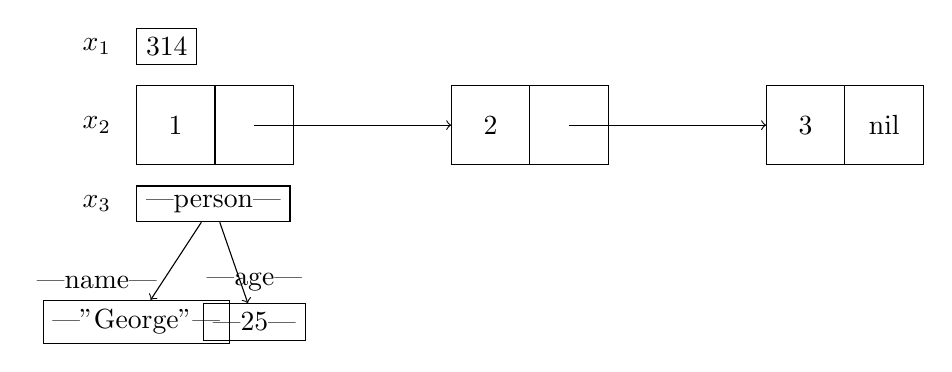
\begin{tikzpicture}
    \draw (0, 0) -- (0, 1) -- (1, 1) -- (1, 0) -- (0, 0);
    \draw (1, 1) -- (2, 1) -- (2, 0) -- (1, 0);
    \node at (0.5, 0.5) {1};

    \draw (4, 0) -- (4, 1) -- (6, 1) -- (6, 0) -- (4, 0);
    \draw (5, 0) -- (5, 1);
    \node at (4.5, 0.5) {2};

    \draw (8, 0) -- (8, 1) -- (10, 1) -- (10, 0) -- (8, 0);
    \draw (9, 0) -- (9, 1);
    \node at (8.5, 0.5) {3};
    \node at (9.5, 0.5) {nil};

    \draw [->] (1.5, 0.5) -- (4, 0.5);
    \draw [->] (5.5, 0.5) -- (8, 0.5);

    \node at (-0.5, 0.5) {$x_2$};
    
    \node at (-0.5, 1.5) {$x_1$};
    \node [right, shape=rectangle, draw] at (0, 1.5) {314};
    
    \node at (-0.5, -0.5) {$x_3$};
    \node (x3) [right, shape=rectangle, draw] at (0, -0.5) {\lstinline|person|};
    \node (George) [shape=rectangle, draw] at (0, -2) {\lstinline|"George"|};
    \node (years_old) [shape = rectangle, draw] at (1.5, -2) {\lstinline|25|};
    \draw [->] (x3) -- (George);
    \draw [->] (x3) -- (years_old);
    \node at (-0.5, -1.5) {\lstinline|name|};
    \node at (1.5, -1.5) {\lstinline|age|  };
\end{tikzpicture}
\caption{Хранилище значений: все переменные привязаны к значениям}
\label{figure:all_variables_bound_to_values}
\end{figure}




В этот момент читатель с некоторым опытом программирования может задаться вопросом: почему мы ввели понятие единого, присваиваемого хранилища, в то время, когда в остальных языках есть хранилища значений или хранилища ячеек. Этому есть много причин. Первая причина --- нам нужно иметь возможность производить вычисления с частичными значениями. Например, процедура может на выходе вернуть привязку к несвязанному аргументу-переменной. Вторая причина --- это декларативный параллелизм, тема Главы 4. Подобный параллелизм возможен благодаря единому, присваиваемому хранилищу. Третья причина --- подобное хранилище является базовым при расширении модели для работы с относительным (логическим) программированием и программированием с ограничениями. Другие причины связаны с эффективностью (например, хвостовая рекурсия и различающиеся списки), рассматриваемой в следующей главе.

\subsection{Создание значения}

Базовой операцией в хранилище является привязка переменной к свеже-созданному значению. Эту операцию мы будем записывать так: $x_{i}=value$ ($x_{i}=\text{\emph{значение}}$). Где $x_{i}$ ссылается непосредственно на переменную в хранилище (и это \emph{не} текстовое имя в программе!) а \emph{value} ссылается на значение, например, 314 или \lstinline|[1 2 3]|. Например, Рис.~\ref{figure:two_variables_bound_to_values} --- это хранилище Рис.~\ref{figure:single-assignment_store_three_unbound_variables} после двух привязок:

\begin{lstlisting}
$x_{1}$ = 314
$x_{2}$ = [1 2 3]
\end{lstlisting}


Операция с единой привязкой $x_{i}$\emph{=value} конструирует \emph{значение value} в хранилище и затем привязывает переменную $x_{i}$ к этому значению. Если переменная уже была привязана, то операция проверит являются ли эти два значения совместимыми. Если они не будут совместимыми, то будет выдан сигнал с ошибкой (используя механизм обработки исключений, смотрите Раздел 2.6).

\subsection{Идентификаторы переменной}

\begin{figure}
  \begin{tikzpicture}
    \draw (1, 1) -- (1, 2) -- (2, 2) -- (2, 1) -- (1, 1);
    \node at (1.5, 1.5) {``X''};

    \draw (7, 0) -- (7, 3) -- (12, 3) -- (12, 0) -- (7, 0);
    \node (x1) at (7.5, 1.5) {$x_{1}$};
    \node [shape=rectangle, draw] at (10, 1.5) {не привязано};
    \node at (1, 2.5) {В определении};
    \node at (9, 2.5 ) {Внутри хранилища};
    \draw [->] (2, 1.5) -- (x1);
  \end{tikzpicture}
\caption{Идентификатор переменной, ссылающейся на непривязанное значение}
\label{figure:referring_to_an_unbound_variable}
\end{figure}


До сих пор мы рассматривали хранилище, которое содержало переменные и значения, то есть, \emph{объекты хранилища}, с которыми мы и выполняли вычисления. Было бы неплохо если бы мы имели возможность ссылаться на объекты хранилища снаружи самого хранилища. Эта роль отведена идентификаторам переменной. \emph{Идентификатор переменной} --- это текстовое имя, ссылающееся на объект хранилища за пределами самого хранилища. Отображение от идентификаторов переменной к объектам хранилища называется \emph{средой}.

Названия переменных в исходном коде программы на самом деле являются идентификаторами переменных. Например, на Рис.~\ref{figure:referring_to_an_unbound_variable} изображён идентификатор ``X'' (заглавная буква X), которая ссылается на переменную хранилища $x_{1}$. Что соответствует среде $\{X \to x_{1}\}$. Для обозначения \emph{любого} идентификатора мы будем использовать запись $\langle x \rangle$. Среда $\{\langle X \rangle \to x_{1}\}$ будет тем же самым что и выше, если $\langle x \rangle$ будет представлять $X$. Как мы увидим позже, идентификаторы переменной и их соответствующие объекты хранилища добавляются в среду через определения \lstinline|local| и \lstinline|declare|.



\subsection{Создание значения с идентификаторами}

\begin{figure}
  \begin{tikzpicture}
    \draw (1, 1) -- (1, 2) -- (2, 2) -- (2, 1) -- (1, 1);
    \node at (1.5, 1.5) {``X''};

    \draw (3, 0) -- (3, 3) -- (12, 3) -- (12, 0) -- (3, 0);
    \node (x1) at (3.5, 1.5) {$x_{1}$};
    \node [shape=rectangle, draw] at (4, 1.5) {};
%    \node at (1, 2.5) {В определении};
    \node at (5, 2.5 ) {Внутри хранилища};
    \draw [->] (2, 1.5) -- (x1);

    \pgfmathsetmacro{\xc}{6};
    \pgfmathsetmacro{\yc}{0.2};
    
    \draw (\xc, \yc) -- (\xc, \yc+0.5) -- (\xc+1, \yc + 0.5) -- (\xc+1, \yc) -- (\xc, \yc);
    \draw (\xc+0.5, \yc+0.5) -- (\xc+0.5, \yc);
    \node at (\xc+0.25, \yc+0.25) {1};

    \draw (\xc+1.5, \yc) -- (\xc+1.5, \yc+0.5) -- (\xc+2.5, \yc + 0.5) -- (\xc+2.5, \yc) -- (\xc+1.5, \yc);
    \draw (\xc+2, \yc+0.5) -- (\xc+2, \yc);
    \node at (\xc+1.75, \yc+0.25) {2};

    \draw (\xc+3, \yc) -- (\xc+3, \yc+0.5) -- (\xc+4, \yc + 0.5) -- (\xc+4, \yc) -- (\xc+3, \yc);
    \draw (\xc+3.5, \yc+0.5) -- (\xc+3.5, \yc);
    \node at (\xc+3.25, \yc+0.25) {3};
    \node at (\xc+3.75, \yc+0.25) {nil};

    \draw [->] (\xc+1, \yc+0.25) -- (\xc+1.5, \yc+0.25);
    \draw [->] (\xc+2.5, \yc+0.25) -- (\xc+3, \yc+0.25);
    \draw [->] (4, 1.5) -- (\xc+0.5, \yc+0.5);
  \end{tikzpicture}
\caption{Идентификатор переменной, ссылающейся на привязанное значение}
\label{figure:identifier_referring_to_a_bound_variable}
\end{figure}

\begin{figure}
  \begin{tikzpicture}
    \draw (1, 1) -- (1, 2) -- (2, 2) -- (2, 1) -- (1, 1);
    \node at (1.5, 1.5) {``X''};

    \draw (3, 0) -- (3, 3) -- (12, 3) -- (12, 0) -- (3, 0);
    \node (x1) at (3.5, 1.5) {$x_{1}$};
%    \node [shape=rectangle, draw] at (4, 1.5) {};
%    \node at (1, 2.5) {В определении};
    \node at (5, 2.5 ) {Внутри хранилища};
    \draw [->] (2, 1.5) -- (x1);

    \pgfmathsetmacro{\xc}{4};
    \pgfmathsetmacro{\yc}{1.25};
    
    \draw (\xc, \yc) -- (\xc, \yc+0.5) -- (\xc+1, \yc + 0.5) -- (\xc+1, \yc) -- (\xc, \yc);
    \draw (\xc+0.5, \yc+0.5) -- (\xc+0.5, \yc);
    \node at (\xc+0.25, \yc+0.25) {1};

    \draw (\xc+1.5, \yc) -- (\xc+1.5, \yc+0.5) -- (\xc+2.5, \yc + 0.5) -- (\xc+2.5, \yc) -- (\xc+1.5, \yc);
    \draw (\xc+2, \yc+0.5) -- (\xc+2, \yc);
    \node at (\xc+1.75, \yc+0.25) {2};

    \draw (\xc+3, \yc) -- (\xc+3, \yc+0.5) -- (\xc+4, \yc + 0.5) -- (\xc+4, \yc) -- (\xc+3, \yc);
    \draw (\xc+3.5, \yc+0.5) -- (\xc+3.5, \yc);
    \node at (\xc+3.25, \yc+0.25) {3};
    \node at (\xc+3.75, \yc+0.25) {nil};

    \draw [->] (\xc+1, \yc+0.25) -- (\xc+1.5, \yc+0.25);
    \draw [->] (\xc+2.5, \yc+0.25) -- (\xc+3, \yc+0.25);
%    \draw [->] (4, 1.5) -- (\xc+0.5, \yc+0.5);
  \end{tikzpicture}
\caption{Идентификатор переменной, ссылающийся на значение}
\label{figure:variable_identifier_referring_to_a_variable}
\end{figure}

Будучи уже привязанной, переменная становится неотличимой от её значения. Рис.~\ref{figure:identifier_referring_to_a_bound_variable} показывает что случится когда $x_{1}$ будет привязан к \lstinline|[1 2 3]| в Рис.~\ref{figure:referring_to_an_unbound_variable}. Пользуясь идентификатором переменной $X$ мы можем описать привязку как \lstinline|$X$=[1 2 3]|. Это текст, который может написать программист для выражения привязки. Также мы можем использовать нотацию \lstinline|$\langle x \rangle$=[1 2 3]| если мы хотим говорить о \emph{любом} идентификаторе. Для того, чтобы эта нотация была корректной в программе, следует заменить $\langle x \rangle$ на конкретный идентификатор.

Знак равенства ``='' относится к операции привязки. После завершения привязки идентификатор ``X'' по-прежнему будет ссылаться на $x_{1}$, который теперь привязан к \lstinline|[1 2 3]|. Ничем не отличается от Рис.~\ref{figure:variable_identifier_referring_to_a_variable}, где $X$ ссылается непосредственно на \lstinline|[1 2 3]|. Следующие ссылки привязанных переменных, используются для получения значения и называются \emph{разыменованием}. Они не видимы для программиста.

\subsection{Частичные значения}

\begin{figure}
  \begin{tikzpicture}
    \draw (1, 1) -- (1, 2) -- (2, 2) -- (2, 1) -- (1, 1);
    \node (X) at (1.5, 1.5) {``X''};

    \draw (3, -2) -- (3, 3) -- (12, 3) -- (12, -2) -- (3, -2);
    \node (x1) at (3.5, 1.5) {$x_{1}$};
%    \node [shape=rectangle, draw] at (4, 1.5) {};
%    \node at (1, 2.5) {В определении};
    \node at (5, 2.5 ) {Внутри хранилища};
    \node (person) [shape = rectangle, draw] at (5, 1.5) {\lstinline|person|};
    \node (George) [shape = rectangle, draw] at (4, 0) {\lstinline|"George"|};
    \node (unbound) [shape = rectangle, draw] at (6, -1) {\lstinline|unbound|};
    \draw [->] (person) -- (George);
    \draw [->] (person) -- (unbound);

    \node at (4, 0.6) {\lstinline|name|};
    \node at (6, -0.4) {\lstinline|age|};

    \node (x2) at (5, -1) {$x_{2}$};

    \node (Y) [shape = rectangle, draw] at (1.5, -1) {``Y''};
    \draw [->] (Y) -- (x2);
    \draw [->] (X) -- (x1);
  \end{tikzpicture}
\caption{Составное значение}
\label{figure:partial_value}
\end{figure}

\begin{figure}
  \begin{tikzpicture}
    \draw (1, 1) -- (1, 2) -- (2, 2) -- (2, 1) -- (1, 1);
    \node (X) at (1.5, 1.5) {``X''};

    \draw (3, -2) -- (3, 3) -- (12, 3) -- (12, -2) -- (3, -2);
    \node (x1) at (3.5, 1.5) {$x_{1}$};
%    \node [shape=rectangle, draw] at (4, 1.5) {};
%    \node at (1, 2.5) {В определении};
    \node at (5, 2.5 ) {Внутри хранилища};
    \node (person) [shape = rectangle, draw] at (5, 1.5) {\lstinline|person|};
    \node (George) [shape = rectangle, draw] at (4, 0) {\lstinline|"George"|};
    \node (unbound) [shape = rectangle, draw] at (6, -1) {\lstinline|25|};
    \draw [->] (person) -- (George);
    \draw [->] (person) -- (unbound);

    \node at (4, 0.6) {\lstinline|name|};
    \node at (6, -0.4) {\lstinline|age|};

    \node (x2) at (5, -1) {$x_{2}$};

    \node (Y) [shape = rectangle, draw] at (1.5, -1) {``Y''};
    \draw [->] (Y) -- (x2);
    \draw [->] (X) -- (x1);
  \end{tikzpicture}
\caption{Частичное значение без несвязанных переменных, то есть, завершённое значение}
\label{figure:complete_value}
\end{figure}

\emph{Частичные значения} --- это структура данных, которая может содержать несвязанные переменные. Рис.~\ref{figure:partial_value} показывает запись \lstinline|person(name:"George"| \lstinline|age:x2)|, на которую ссылается идентификатор \lstinline|X|. Частичным оно является потому, что содержит несвязанную переменную $x_{2}$. Идентификатор \lstinline|Y| ссылается на $x_{2}$. Рис.~\ref{figure:complete_value} иллюстрирует ситуацию после того, как $x_{2}$ привязан к 25 (с помощью операции привязки \lstinline|Y=25|). Теперь $x_{1}$ частичное значение без несвязанных переменных, теперь мы можем назвать $x_{1}$ \emph{завершённым значением}. Декларативная переменная может быть привязана к нескольким частичным значениям, так долго, насколько они будут оставаться совместимыми друг с другом. Мы называем набор частичных значений \emph{совместимыми}, если эти значения могут входить в несвязанные переменные так, что эти переменные будут равны друг другу. Например, \lstinline|person(age:25)| и \lstinline|person(age:x)| совместимы (поскольку $x$ может быть привязан к 25), но \lstinline|person(age:25)| и \lstinline|person(age:26)| не совместимы.


\subsection{Привязка переменная-переменная}

\begin{figure}
  \begin{tikzpicture}
    \draw (1, 1) -- (1, 2) -- (2, 2) -- (2, 1) -- (1, 1);
    \node (X) at (1.5, 1.5) {``X''};

    \draw (3, -2) -- (3, 3) -- (12, 3) -- (12, -2) -- (3, -2);
    \node (x1) at (3.5, 1.5) {$x_{1}$};
    \node (x2) at (3.5, -1) {$x_{2}$};
%    \node [shape=rectangle, draw] at (4, 1.5) {};
%    \node at (1, 2.5) {В определении};
    \node at (5, 2.5 ) {Внутри хранилища};
    \node (Y) [shape = rectangle, draw] at (1.5, -1) {``Y''};
    \pgfmathsetmacro{\xc}{4};
    \pgfmathsetmacro{\yc}{1.25};
    \draw (\xc, \yc) -- (\xc, \yc + 0.5) -- (\xc + 3, \yc + 0.5) -- (\xc + 3, \yc) -- (\xc, \yc);

    \pgfmathsetmacro{\ys}{-1.25};
    \draw (\xc, \ys) -- (\xc, \ys + 0.5) -- (\xc + 3, \ys + 0.5) -- (\xc + 3, \ys) -- (\xc, \ys);

    %    \draw ((4 + 3)/2, (\yc + 0.5)/2) .. controls ((\xc + 3)/2 - 1, (\yc + \ys)/2) .. ((\xc + 3)/2, \ys + 0.5);
    \draw [->] (\xc+1.5, \yc + 0.25) .. controls (\xc + 1, 0) .. (\xc + 1.5, \ys + 0.5);
    \draw [->] (\xc+1.5, \ys + 0.25) .. controls (\xc+2, 0) .. (\xc+1.5, \yc);
    \draw [->] (X) -- (x1);
    \draw [->] (Y) -- (x2);
  \end{tikzpicture}
\caption{Две переменные связаны вместе}
\label{figure:two_variables_bound_together}
\end{figure}

\begin{figure}
  \begin{tikzpicture}
    \draw (1, 1) -- (1, 2) -- (2, 2) -- (2, 1) -- (1, 1);
    \node (X) at (1.5, 1.5) {``X''};

    \draw (3, -2) -- (3, 3) -- (12, 3) -- (12, -2) -- (3, -2);
    \node (x1) at (3.5, 1.5) {$x_{1}$};
    \node (x2) at (3.5, -1) {$x_{2}$};
%    \node [shape=rectangle, draw] at (4, 1.5) {};
%    \node at (1, 2.5) {В определении};
    \node at (5, 2.5 ) {Внутри хранилища};
    \node (Y) [shape = rectangle, draw] at (1.5, -1) {``Y''};
    \pgfmathsetmacro{\xc}{4};
    \pgfmathsetmacro{\yc}{1.25};
    \draw (\xc, \yc) -- (\xc, \yc + 0.5) -- (\xc + 3, \yc + 0.5) -- (\xc + 3, \yc) -- (\xc, \yc);

    \pgfmathsetmacro{\ys}{-1.25};
    \draw (\xc, \ys) -- (\xc, \ys + 0.5) -- (\xc + 3, \ys + 0.5) -- (\xc + 3, \ys) -- (\xc, \ys);

    %    \draw ((4 + 3)/2, (\yc + 0.5)/2) .. controls ((\xc + 3)/2 - 1, (\yc + \ys)/2) .. ((\xc + 3)/2, \ys + 0.5);
    %\draw [->] (\xc+1.5, \yc + 0.25) .. controls (\xc + 1, 0) .. (\xc + 1.5, \ys + 0.5);
    %\draw [->] (\xc+1.5, \ys + 0.25) .. controls (\xc+2, 0) .. (\xc+1.5, \yc);
    \draw [->] (X) -- (x1);
    \draw [->] (Y) -- (x2);

    \pgfmathsetmacro{\xv}{6};
    \pgfmathsetmacro{\yv}{0};
    
    \draw (\xv, \yv) -- (\xv, \yv+0.5) -- (\xv+1, \yv + 0.5) -- (\xv+1, \yv) -- (\xv, \yv);
    \draw (\xv+0.5, \yv+0.5) -- (\xv+0.5, \yv);
    \node at (\xv+0.25, \yv+0.25) {1};

    \draw (\xv+1.5, \yv) -- (\xv+1.5, \yv+0.5) -- (\xv+2.5, \yv + 0.5) -- (\xv+2.5, \yv) -- (\xv+1.5, \yv);
    \draw (\xv+2, \yv+0.5) -- (\xv+2, \yv);
    \node at (\xv+1.75, \yv+0.25) {2};

    \draw (\xv+3, \yv) -- (\xv+3, \yv+0.5) -- (\xv+4, \yv + 0.5) -- (\xv+4, \yv) -- (\xv+3, \yv);
    \draw (\xv+3.5, \yv+0.5) -- (\xv+3.5, \yv);
    \node at (\xv+3.25, \yv+0.25) {3};
    \node at (\xv+3.75, \yv+0.25) {nil};
    \draw [->] (\xv+1, \yv+0.25) -- (\xv+1.5, \yv+0.25);
    \draw [->] (\xv+2.5, \yv+0.25) -- (\xv+3, \yv+0.25);


    \draw [->] (\xc+1.5, \yc + 0.25) -- (\xv + 0.5, \yv + 0.5);
    \draw [->] (\xc+1.5, \ys + 0.25) -- (\xv+0.5, \yv);

  \end{tikzpicture}
\caption{Хранилище после привязки одного из переменных}
\label{figure:after_binding_one_of_the_variable}
\end{figure}

Переменные могут привязываться к переменным. Например, рассмотрим две несвязанные переменные $x_{1}$ и $x_{2}$, на которые ссылаются идентификаторы \lstinline|X| и \lstinline|Y|. После выполнения привязки \lstinline|X=Y| мы получаем ситуацию, проиллюстрированную на Рис.~\ref{figure:two_variables_bound_together}. Две переменные $x_{1}$ и $x_{2}$ равны друг другу. На картинке это изображено через взаимные ссылки переменных. Мы говорим что форма $\{x_{1}, x_{2}\}$ образует \emph{эквивалентное множество}.\footnote{С формальной точки зрения, две переменные образуют класс эквивалентности по отношению к равенству.} Что в свою очередь записывается как $x_{1}=x_{2}$. Три переменные, связанные вместе будут записываться как $x_{1}=x_{2}=x_{3}$ или $\{x_{1}, x_{2}, x_{3}\}$. Если изобразить это в рисунке, то эти переменные сформируют закольцованную цепочку. Вне зависимости от того к чему будет привязана какая-либо переменная в эквивалентности, все остальные переменные увидят эти привязки. Рис.~\ref{figure:after_binding_one_of_the_variable} показывает результат выполнения \lstinline|X=[1 2 3]|.

\subsection{Переменные с потоком данных}\label{subsection:dataflow_variables}

В декларативной модели \emph{создание} переменной и её \emph{привязка} --- различные операции. Что произойдёт если попытаться использовать переменную ещё до привязки? Мы называем такой случай \emph{ошибкой использования переменной}. Некоторые языки создают и связывают переменные за один шаг, таким образом не возникает ошибки использования. Такой подход характерен для функциональных языков программирования. Другие языки позволяют разделять операции создания и привязки. Дальше у нас возможны следующие варианты развития событий при ошибке использования:

\begin{enumerate}
  
\item{Работа программы продолжается и не выдаётся предупреждение об ошибке. Содержимое переменной не определено, то есть, ``мусор'': что был в памяти. Характерно для C++.}

\item{Работа программы продолжается и не выдаётся предупреждение об ошибке. Переменная инициализируется значением по-умолчанию при объявлении переменной, например, 0 для целых чисел. Характерно для Java.}

\item{Работа программы прекращается с сообщением об ошибке (или генерируется исключение). Характерно для Prolog при работе с арифметическими операциями.}

\item{Работа программы приостанавливается до тех пор, пока переменная не будет привязана, после чего работа продолжается.}
\end{enumerate}

Варианты упорядочены по возрастанию правильности поведения. Крайне плохим является первый вариант, поскольку несколько запусков программы могут дать различные результаты. И что ещё хуже --- так это то, что не создаётся сообщение об ошибке, программист может даже не понять что произошло. Второй вариант немного получше. Если в программе была допущена ошибка использования, то по крайней мере, программа всегда будет возвращать один результат, даже если он не верный. И опять программист не уведомлен о существовании ошибки.

Третий и четвёртый варианты допустимы в некоторых ситуациях. В третьем варианте программа с ошибкой использования не будет молчать и даст сигнал. Такое поведение допустимо для последовательных систем, поскольку, в самом деле, является ошибкой. И не допустимо для параллельных систем поскольку результат становится не детерминированным: зависит от обстоятельств, иногда возникает ошибка, иногда нет. В четвёртом варианте программа будет ждать пока переменная не будет привязана, после чего продолжит работу. Это недопустимо для последовательных систем, поскольку программа будет ждать привязки вечно. И допустимо для параллельных систем, где такое поведение может быть частью нормальной работы, например, когда один тред связывает переменную.\footnote{Но, при разработке, хороший отладчик должен обнаруживать нежелательные зависания при отсутствии других запущенных тредов.} Вычислительная модель, использованная в этой книге, использует четвёртый вариант.


Декларативные переменные, приостанавливающие работу программы до тех пор, пока эти переменные они не будут связанными, называются переменными \emph{потоков данных}. Декларативная модель, использующая переменные потоков данных, чрезвычайно удобна в параллельном программировании, то есть, для программ, исполняемых независимо. Если мы выполняем две параллельные операции, скажем \lstinline|A=23| и \lstinline|B=A+1|, то четвёртое решение всегда будет срабатывать корректно и давать ответ \lstinline|B=24|. И не важно, что будет срабатывать первым: \lstinline|A=23| или \lstinline|B=A+1|. В случае с остальными вариантами у нас нет такой гарантии. Такая \emph{потоко-независимая} особенность делает возможным декларативный параллелизм в Главе 4. В этом заключается вся соль переменных потоков данных.

\section{Язык ядра}\label{section:kernel_language}






Декларативная модель определяет простой язык ядра. Все программы, находящиеся в рамках этой модели, могут быть выражены этим языком. Первым делом мы опишем синтаксис языка ядра и его семантику. Затем мы опишем как следует построить полноценный язык на основе языка ядра.

\subsection{Синтаксис}

\begin{table}

  \begin{tabular}{|ll|}
    \hline
    \lstinline|$\langle$s$\rangle$ ::=| & \\
    \lstinline|  skip| & Пустое определение\\
    \lstinline! |${\langle s \rangle}_{1}$ ${\langle s \rangle}_{2}$! & Последовательность определения\\
    \lstinline! |local $\langle x \rangle$ in $\langle s \rangle$ end! & Создание переменной\\
    \lstinline! |${\langle x \rangle}_{1}$=${\langle x \rangle}_{2}$! & Привязка переменная-переменная\\
    \lstinline! |${\langle x \rangle}$=${\langle v \rangle}$! & Создание значения\\
    \lstinline! |if $\langle x \rangle$ then ${\langle s \rangle}_{1}$ else ${\langle s \rangle}_{2}$ end! & Условие\\
    \lstinline! |case $\langle x \rangle$ of $\langle pattern \rangle$ then ${\langle s \rangle}_{1}$ else ${\langle s \rangle}_{2}$ end! & Сравнение по шаблону\\
    \lstinline! |$\{\langle x \rangle {\langle y \rangle}_{1} ... {\langle y \rangle}_{n}\}$! & Применение процедуры\\
    \hline
  \end{tabular}
  
\caption{Декларативный язык ядра}
\label{table:the_declarative_kernel_language}
\end{table}

\begin{table}
  \begin{tabular}{|lrl|}
    \hline
    \lstinline|$\langle v \rangle$| & ::= & \lstinline!$\langle number \rangle$|$\langle record \rangle$|$\langle procedure \rangle$!\\
    \lstinline|$\langle number \rangle$| & ::= & \lstinline!$\langle int \rangle$|$\langle float \rangle$!\\
    \lstinline|$\langle record \rangle$, $\langle pattern \rangle$| & ::= & \lstinline!$\langle literal \rangle$!\\
    \lstinline| | & | & \lstinline!$\langle literal \rangle ({\langle feature \rangle}_{1}:{\langle x \rangle}_{1} ... {\langle feature \rangle}_{n}:{\langle x \rangle}_{n})$!\\
    \lstinline|$\langle procedure \rangle$| & ::= & \lstinline!proc {$\$$ ${\langle x \rangle}_{1} ... {\langle x \rangle}_{n}$} $\langle s \rangle$ end!\\
    \lstinline|$\langle literal \rangle$| & ::= & \lstinline!$\langle atom \rangle$|$\langle bool \rangle$!\\
    \lstinline|$\langle feature \rangle$| & ::= & \lstinline!$\langle atom \rangle$|$\langle bool \rangle$|$\langle int \rangle$!\\
    \lstinline|$\langle bool \rangle$| & ::= & \lstinline!true | false!\\
    \hline
  \end{tabular}
  
\caption{Выражение значений в декларативном языке ядра}
\label{table:value_expressions_kernel_language}
\end{table}

Синтаксис ядра показан в Таблицах \ref{table:the_declarative_kernel_language} и \ref{table:value_expressions_kernel_language}. Этот синтаксис спроектирован так, чтобы быть подмножеством синтаксиса полноценного языка, то есть, все операторы языка ядра являются корректными операторами полноценного языка.

\subsubsection{Синтаксис определения}

Таблица \ref{table:the_declarative_kernel_language} определяет синтаксис $\langle s \rangle$, обозначающий определение. Всего существует восемь определений, о которых мы поговорим позже.

\subsubsection{Синтаксис значения}

Таблица \ref{table:value_expressions_kernel_language} определяет синтаксис $\langle v \rangle$, что обозначает значение. Существует три разновидности выражения значения, это числа, записи и процедуры. Для записей и шаблонов, все аргументы $\langle x \rangle$, ..., ${\langle x \rangle}_{n}$ должны быть различными идентификаторами. Такой подход позволяет с уверенностью говорить о том, что все привязки переменная-переменная написаны в явных операциях ядра.

\subsubsection{Синтаксис идентификатора переменной}

Таблица \ref{table:the_declarative_kernel_language} использует нетерминалы $\langle x \rangle$ и $\langle y \rangle$ для обозначения идентификатора переменной. Кроме того, для обозначения идентификаторов мы будем использовать $\langle z \rangle$. Есть два способа написать идентификатор переменной:

\begin{itemize}
\item{Буква в верхнем регистре, со следующими за ней от нуля и более цифровыми и буквенными символами, например, \lstinline|X|, \lstinline|X1| \\или \lstinline|ThisIsALongVariablentIt|.}

\item{Любая последовательность печатаемых символов, окружённая символом $'$ (обратная кавычка), например, $'$\verb|this is a 25$\variable!|$'$.}
\end{itemize}

Точное определение синтаксиса идентификатора дано в Приложении C. Все свежесозданные переменные не привязываются до тех пор пока выполняется определение. Все идентификаторы переменных должны определяться явно.

\subsection{Значения и типы}

\emph{Тип} или \emph{тип данных} --- это набор значений плюс набор операций, выполняемых с этими значениями. Значение ``относится к типу'' если находится во множестве этого типа. Декларативная модель \emph{типизирована} в некотором множестве ранее определённых типов, называемых \emph{базовыми типами}. Например, программы могут вычисляться через целые числа или через записи, соответственно относящиеся к целочисленному типу или к типу записи. Любая попытка применить некорректную операцию к какому-либо типу будет определена системой и приведёт к возникновению ошибочного состояния (смотрите Раздел 2.6). Модель не накладывает никаких других ограничений на использование этих типов.

Поскольку все типы проверяются, то исключается какое-либо поведение за пределом модели, например, прекращение работы программы по причине неопределённых операций во внутренней структуре данных. Но, не исключено возникновение ошибочных состояний, например, деление на ноль. В декларативной модели, программы, столкнувшиеся с ошибочными состояниями будут немедленно завершены. В модели нет никаких средств для обработки ошибок. В Разделе 2.6 мы расширяем декларативную модель новой концепцией, \emph{исключениями}, что позволит нам обрабатывать ошибки. В расширенной модели, ошибки типов могут быть обработаны внутри модели.

В дополнение к базовым типам программы могут определять свои собственные типы, которые называются \emph{абстрактными типами данных (abstract data types)}, сокращённо ADT. Глава 3 и остальные главы показывают как определять ADT.

\subsubsection{Базовые типы}

Базовыми типами декларативной модели являются числа (целочисленные и плавающие), записи (включая атомы, булевы значения, кортежи, списки и строки) и процедуры. В Таблице \ref{table:value_expressions_kernel_language} описывается их синтаксис. Нетерминал $\langle v \rangle$ обозначает частично сконструированное значение. Позже, по мере чтения книги мы познакомимся с другими базовыми типами, включая чанки (chunks), функторы, ячейки, словари, массивы, порты, классы и объекты. Некоторые из них описаны в Приложении B.

\subsubsection{Динамическая типизация}

Существует два базовых подхода к типизации, а именно: динамическая и статическая типизация. В статической типизации все типы переменных известны во время компиляции. В динамической типизации тип переменной становится известным только во время привязки. Декларативная модель является динамически типизированной. Компилятор пытается проверить что все операции используют корректные типы. Но, поскольку мы имеем дело с динамической типизацией, некоторые проверки типов выполняются во время работы программы.

\subsubsection{Иерархия типов}

\begin{figure}
\begin{tikzpicture}
  \node (value) {Значение};
  \node [below left = 1cm and 3cm of value] (number) {Число};
  \node [below left = 1cm and 0.5cm of value] (record) {Запись};
  \node [below right = 1cm and 0cm of value] (procedure) {Процедура};
  \node [below right = 1cm and 3cm of value] (firstdots) {...};
  \draw [->] (value) -- (number);
  \draw [->] (value) -- (record);
  \draw [->] (value) -- (procedure);
  \draw [->] (value) -- (firstdots);
  \node [below = 0.5cm of procedure] (seconddots) {...};

  \node [below left = 0.5cm and 0.5cm of number] (int) {Целое};
  \node [below  = 0.5cm of number] (float) {Плавающее};
  \draw [->] (number) -- (int);
  \draw [->] (number) -- (float);
  
  \node [below = 0.5cm of int] (char) {Символ};
  \draw [->] (int) -- (char);
  
  \node [below = 0.5cm of record] (tuple) {Кортеж};
  \draw [->] (record) -- (tuple);
  
  \node [below left = 1cm and 0.5cm of tuple] (literal) {Литерал};
  \node [below left = 0.5cm and 0.5cm of literal] (bool) {Булево};
  \node [below left = 0.5cm and 0.5cm of bool] (true) {Истина};
  \node [below = 0.5cm of bool] (false) {Ложь};


  
  \node [below = 0.5cm of literal] (atom) {Атом};
  \node [below right = 0.5cm and 0.5cm of literal] (fourthdots) {...};
  
  \node [below right = 1cm and 0.1cm of tuple] (list) {Список};
  \node [below right = 0.5cm and 1.5cm of tuple] (thirddots) {...};
  \node [below = 0.5cm of list] (string) {Строка};
  \draw [->] (tuple) -- (literal);
  \draw [->] (tuple) -- (list);
  \draw [->] (tuple) -- (thirddots);
  \draw [->] (literal) -- (bool);
  \draw [->] (literal) -- (atom);
  \draw [->] (literal) -- (fourthdots);
  \draw [->] (bool) -- (true);
  \draw [->] (bool) -- (false);
  \draw [->] (list) -- (string);
  \draw [->] (procedure) -- (seconddots);
\end{tikzpicture}
\caption{Иерархия типов декларативной модели}
\label{figure:declarative_model_type_hierarchy}
\end{figure}

Базовые типы декларативной модели можно классифицировать как иерархию. Рис.~\ref{figure:declarative_model_type_hierarchy} иллюстрирует эту иерархию, где каждый узел обозначает тип. Иерархия упорядочена по \emph{вхождению множества}, то есть, все значения типа узла также являются значениями родителя типа узла. Например, все кортежи --- это записи и все списки --- это кортежи. Это значит что все операции типа приемлемы для подтипа, например, все списковые операции будут работать и со строками. Позже мы расширим эту иерархию. Например, все литералы могут быть либо атомами (описано ниже), либо другой разновидностью с постоянными названиями (смотрите Раздел 3.7.5). Участки с незавершённой иерархией отмечены как ``...''.


\subsection{Базовые типы}\label{subsection:basic_types}

Здесь мы дадим некоторые примеры базовых типов и их написание. Более полная информация содержится в Приложении B.

\begin{itemize}

\item{\textbf{Числа}. Числа бывают либо целочисленные, либо с плавающей запятой. Примеры целочисленных значений: \lstinline|314|, \lstinline|0| и \lstinline|~10| (минус 10). Заметьте, что символ минуса записан тильдой ``\lstinline|~|''. Примеры чисел с плавающей запятой: \lstinline|1.0|, \lstinline|3.4|, \lstinline|2.02e2| и \lstinline|~2.02E~2|.}

\item{\textbf{Атомы}. Атом --- это разновидность символьной константы, которая может быть использована как отдельный элемент в вычислениях. Есть несколько способов записи атомов. Атом может быть записан как последовательность символов, начинающихся с буквы в нижнем регистре с последующим произвольным количеством букв и цифр. Кроме того, атом может быть записан как произвольная последовательность печатаемых символов, окружённая одинарными кавычками. Примеры атомов: \lstinline|a_person|, \lstinline|donkeyKong3| и \lstinline|$'$#### hello ####$'$|.}

\item{\textbf{Булевы значения}. Булево значение может быть либо символом \lstinline|true|, либо символом \lstinline|false|.}

\item{\textbf{Записи}. Запись --- это составная структура данных. Она состоит из метки с последующим набором пар идентификаторов свойств и значений. Свойства могут быть атомами, целыми числами или булевыми значениями. Примеры записей: \lstinline|person(age:X1 name:X2)| (со свойствами \lstinline|age| и \lstinline|name|),  \lstinline|person(1:X1 2:X2)|,  \lstinline!$'$|$'$ (1:H 2:T)!, \lstinline!$'$#$'$ (1:H 2:T)!, \lstinline|nil| и \lstinline|person|. Атом --- это запись без свойств.}
%\end{itemize}

\item{\textbf{Кортежи}. Кортеж --- это запись, свойствами которой являются последовательные числа, начинающиеся с 1. В данном случае свойства не указываются. Примеры кортежей: \lstinline|person(1:X1 2:X2)| и \lstinline|person(X1 X2)|, эти оба кортежа обозначают одно и то же.}

\item{\textbf{Списки}. Список может быть либо атомом \lstinline|nil|, либо кортежем  \lstinline!$'$|$'$ (H T)! (меткой является вертикальная черта), где \lstinline|T| либо привязан к списку, либо нет. Этот кортеж называется \emph{списковой парой} или \emph{cons}. Для списков имеется синтаксический сахар:

  \begin{itemize}
  \item{Метка  \lstinline!$'$|$'$!  может быть записана как инфиксный оператор, поэтому \lstinline!H|T! обозначает то же самое, что и  \lstinline!$'$|$'$ (H|T)!.}
    
  \item{Оператор  \lstinline!$'$|$'$!  ассоциирован направо, поэтому \lstinline!1|2|3|nil! обозначает то же самое, что и \lstinline!1|(2|(3|nil))!.}
    
\item{Списки, заканчивающиеся на \lstinline|nil| могут быть записаны с помощью квадратных скобок \lstinline|[ ... ]|, таким образом \lstinline|[1 2 3]| означает то же самое, что и \lstinline!1|2|3|nil!. Такие списки называются \emph{завершёнными списками}.}
  \end{itemize}}
  
\item{\textbf{Строки}. Строка --- это список, состоящий из кодов символов. Строки могут записываться с помощью двойных кавычек, таким образом \lstinline|"E=mc^2"| означает то же самое, что и \lstinline|[69 61 109 99 94 50]|.}
%\end{itemize}

\item{\textbf{Процедуры}. Процедура --- это значение с типом процедуры. Определение:

  \begin{quote}
    \lstinline|$\langle$x$\rangle$=proc {$\$$ ${\langle y \rangle}_{1}$ ... ${\langle y \rangle}_{n}$ } $\langle s \rangle$ end|
  \end{quote}
  
привязывает \lstinline|$\langle x \rangle$| к новому значению процедуры. То есть, просто определяется новая процедура. Символ $\$$ обозначает что значение процедуры является анонимным, то есть, создано без привязки к идентификатору. Существует более знакомое синтаксическое сокращение:

\begin{quote}
  \lstinline|proc { $\langle x \rangle {\langle y \rangle}_{1}$ ... ${\langle y \rangle}_{n}$ } $\langle s \rangle$ end|
\end{quote}

Символ $\$$ замещается идентификатором. Создаётся значение процедуры и немедленно производится попытка привязать его к $\langle x \rangle$. Возможно это сокращение удобно читать, но оно размывает разницу между созданием значения и привязкой значения к идентификатору.}
\end{itemize}

\subsection{Записи и процедуры}

Мы объясним по какой причине записи и процедуры были включены в состав базовых концепций в язык ядра. Этот раздел предназначен для читателей с некоторым опытом в программировании, которых удивляют наши архитектурные решения языка ядра.

\subsubsection{Мощь записей}

Записи --- это базовый способ структурирования данных. В Главе 3 мы увидим что записи --- это строительный материал для большинства структур данных включая списки, деревья, очереди, графы и так далее. Записи играют примерно такую же роль и в большинстве других языках программирования. Но мы увидим, что их мощь может пойти дальше этой роли. Дополнительная мощь зачастую зависит от степени поддержки записей в том или ином языке программирования. Для максимальной мощи язык должен позволять с лёгкостью создавать записи, работать с частями записи и манипулировать ими. В декларативной модели запись создаётся простым и удобным компактным синтаксисом. Часть записи можно получить создав простой шаблон, также обладающий компактным синтаксисом. И наконец, есть много операций для манипуляции записями: добавление, удаление или выбор полей, конвертация в списки и обратно и так далее. В целом, язык осуществляющий подобный уровень поддержки записей называется \emph{символическим (symbolic)} языком.

Если записи хорошо поддерживаются языком, то они (записи) могут использоваться для повышения эффективности множества других техник. Эта книга сфокусирована на трёх техниках: объектно - ориентированное программирование, архитектура графического интерфейса пользователя (GUI) и компонентное программирование. В Главе 7, посвящённой объектно-ориентированному программированию, показано как записи могут представлять сообщения и методы, используемые объектами для взаимодействия. В Главе 10, посвящённой архитектуре GUI, показано как записи могут представлять ``виджеты'', базовые строительные блоки для пользовательского интерфейса. В компонентном программировании, Раздел 3.9, показано как записи могут представлять модули, группирующиеся вместе связанными операциями.

\subsubsection{Почему процедуры?}

Читатель, обладающий некоторым опытом программирования, может задаться вопросом: почему процедуры входят в наш язык ядра как базовые конструкции? Любители объектно-ориентированного программирования могут спросить: почему бы для этого не применить объекты? Любители функционального программирования спросят: а почему использованы именно процедуры, а не функции? Мы могли выбрать любой вариант, но почему остановились именно на процедурах? Причины достаточно очевидны.

Процедуры проще объектов, поэтому процедуры предпочтительнее. Объекты достаточно усложнены, смотрите Главу 7. Процедуры не обязательно определяют такие сущности, как математические функции, поэтому процедуры предпочтительнее функций.\footnote{С теоретической точки зрения, процедуры --- это ``процессы'', используемые в таких параллельных исчислениях, как $\pi$ исчисление. Аргументы --- это каналы. В этой главе мы используем последовательно составленные процессы с одиночным каналом. Главы 4 и 5 показывают другие разновидности каналов (с последовательностями сообщений) и осуществляют параллельную композицию процессов.} Например, на основе процедур мы определяем функции и объекты как абстракции. В дополнение, процедуры гибки поскольку процедуры не делают никаких допущений по числу введённых и выведенных данных. Функция всегда даёт на выходе одно значение. Процедура может иметь на входе и выходе любое количество значений, включая ноль. Мы увидим, что процедуры --- это чрезвычайно мощные строительные блоки, когда будем говорить о высокоуровневом программировании в Разделе 3.6.

\subsection{Базовые операции}

\begin{table}
  \begin{tabular}{|lll|}
    \hline
    Операция & Описание & Тип аргумента\\
    \hline
    \lstinline|A==B| & Проверка на равенство & Значение\\
    \lstinline|A\=B| & Проверка на неравенство & Значение\\
    \lstinline|{IsProcedure P}| & Проверка на процедуру & Значение\\
    \lstinline|A=<B| & Проверка на меньше чем либо равно & Число или Атом\\
    \lstinline|A<B| & Проверка на меньше чем & Число или Атом\\
    \lstinline|A>=B| & Проверка на больше либо равно & Число или Атом\\
    \lstinline|A>B| & Проверка на больше & Число или Атом\\
    \lstinline|A+B| & Сложение & Число\\
    \lstinline|A-B| & Вычитание & Число\\
    \lstinline|A*B| & Умножение & Число\\
    \lstinline|A div B| & Целочисленное деление & Целое число\\
    \lstinline|A mod B| & Остаток от деления & Целое число\\
    \lstinline|A/B| & Деление & Число с плавающей запятой\\
    \lstinline|{Arity R}| & Арность & Запись\\
    \lstinline|{Label R}| & Метка & Запись\\
    \lstinline|R.F| & Выбор поля & Запись\\
    \hline
  \end{tabular}
  
\caption{Примеры базовых операций}
\label{table:examples_of_basic_operations}
\end{table}

В таблице \ref{table:examples_of_basic_operations} проиллюстрированы базовые операции, которые мы будем использовать в этой и последующих главах. Для многих из них есть синтаксический сахар, поэтому они могут быть записаны как выражения. Например, \lstinline|X=A*B| --- это синтаксический сахар для  \lstinline|{Number.$'$*$'$ A B X}|, где  \lstinline|Number.$'$*$'$|  --- это процедура, ассоциированная для типа \lstinline|Number.|\footnote{Если быть точным, \lstinline|Number| --- это модуль в котором сгруппированы операции над типом \lstinline|Number| и \lstinline|Number.$'$*$'$| выбирает операцию умножения.} Все операции могут быть записаны подобной длинной записью, например,  \lstinline|Value.$'$==$'$|, \lstinline|Value.$'$<$'$|, \lstinline|Int.$'$div$'$|, \lstinline|Float.$'$/$'$|. В таблице используется синтаксический сахар везде, где только он есть.

\begin{itemize}

\item{\textbf{Арифметика}. Числа с плавающей запятой обладают четырьмя базовыми операциями: \lstinline|+|, \lstinline|-|, \lstinline|*| и \lstinline|/|, с их обычными значениями. Целые числа обладают базовыми операциями \lstinline|+|, \lstinline|-|, \lstinline|*|, \lstinline|div| и \lstinline|mod|, где \lstinline|div| --- это целочисленное деление (остаток отбрасывается) и \lstinline|mod| --- остаток от деления. Например, \lstinline|10 mod 3 = 1|.}

\item{\textbf{Операции над записями}. Над записями существуют три базовые операции: \lstinline|Arity|, \lstinline|Label| и ``\lstinline|.|'' (точка, обозначает выбор поля). Например, дано следующее:

  \begin{quote}
\lstinline|X=person(name:"George"| \lstinline|age:25)|
  \end{quote}
  
здесь \lstinline|{Arity X}=[age name]|, \lstinline|{Label X} = person| и \lstinline|X.age=25|. Вызов \lstinline|Arity| возвращает список, содержащий: первое, целые свойства в порядке возврастания и, второе, атомы свойств, в порядке возрастания по алфавиту.}

\item{\textbf{Сравнения}. Булевы функции сравнения включают в себя \lstinline|==| и \lstinline|\=|, которые могут сравнивать два значения на равенство, также, числовые сравнения \lstinline|=<|, \lstinline|<|, \lstinline|>=| и \lstinline|>|, которые могут сравнивать два целых значения, два значения с плавающей запятой или два атома. Атомы сравниваются в соответствии их алфавитному порядку при печати. В следующем примере, \lstinline|Z| привязывается к максимуму из \lstinline|X| и \lstinline|Y|.

  \begin{lstlisting}
declare X Y Z T in
X=5 Y=10
T=(X>=Y)
if T then Z=X else Z=Y end
  \end{lstlisting}
  
Для \lstinline|if| есть синтаксический сахар, который позволяет использовать выражение как условие. Вышеприведённый пример можно переписать так:

\begin{lstlisting}
declare X Y Z in
X=5 Y=10
if X>=Y then Z=X else Z=Y end
\end{lstlisting}
}
  
\item{\textbf{Процедурные операции}. Над процедурами можно выполнять три базовые операции: определять их (с помощью оператора \lstinline|proc|), вызывать их (в записи с фигурными скобками) и проверять является ли значение процедурой с помощью функции \lstinline|IsProcedure|. Вызов \lstinline|{IsProcedure P}| вернёт \lstinline|true| если \lstinline|P| является процедурой, в противном случае будет возвращено \lstinline|false|.}
\end{itemize}

В приложении B дан более полный набор базовых операций.

\section{Семантика языка ядра}

Исполнение языка ядра состоит из вычисления функций над частичными значениями. Для того, чтобы увидеть это мы дадим семантику языка ядра в терминах простой операционной модели. Модель спроектирована так, чтобы дать программисту возможность просто рассуждать о корректности и сложности. Это разновидность абстрактной машины, но с высокоуровневой абстракцией, отбрасывающей такие детали как регистры и точную адресацию памяти.

\subsection{Базовые концепции}\label{subsection:basic_concepts}

Прежде чем приступить к формальной семантике, позвольте уделить внимание тому, как выполняется язык ядра. Это позволит стимулировать изучение семантики и упростит её понимание.

\subsubsection{Простое исполнение}

При нормальном исполнении, операторы выполняются один за другим в порядке их появления в тексте. Рассмотрим простое исполнение:

\begin{lstlisting}
local A B C D in
   A=11
   B=2
   C=A+B
   D=C*C
end
\end{lstlisting}

Выглядит довольно просто; \lstinline|D| привязывается к 169. Рассмотрим подробнее происходящие процессы. Оператор \lstinline|local| создаёт четыре новых переменных в хранилище и делает так, чтобы идентификаторы \lstinline|A|, \lstinline|B|, \lstinline|C|, \lstinline|D| ссылались на эти переменные. (Оператор \lstinline|local| приведён в Таблице \ref{table:the_declarative_kernel_language}). Далее следуют две привязки, \lstinline|A=11| и \lstinline|B=2|. Сложение \lstinline|C=A+B| складывает значения \lstinline|A| и \lstinline|B| и привязывает \lstinline|C| к результату \lstinline|13|. В следующей операции, происходит умножение значения \lstinline|C| на своё же значение и \lstinline|D| привязывается к получившемуся результату 169. Достаточно просто.

\subsubsection{Идентификаторы переменных и статическая область видимости}

Мы видим, что оператор \lstinline|local| выполняет две вещи: создаёт новую переменную и делает так, чтобы идентификатор ссылался на переменную. Идентификатор ссылается на переменную только внутри оператора \lstinline|local|, то есть, между \lstinline|local| и \lstinline|end|. Это явление мы называем \emph{областью видимости} идентификатора. За пределами этой области идентификатор не будет означать то же самое. Рассмотрим происходящие процессы подробнее. Взглянем на следующий фрагмент:

\begin{lstlisting}
local X in
   X=1
   local X in
      X=2
      {Browse X}
   end
   {Browse X}
end
\end{lstlisting}

Что будет напечатано при выполнении этой программы? При выполнении этой программы вначале будет напечатано 2, а затем 1. В данном случае мы имеем дело всего лишь с одним идентификатором \lstinline|X|, но, в различных этапах работы это идентификатор будет ссылаться на различные переменные.

Подведём итоги этой идеи. Значение такого идентификатора как \lstinline|X| определяется вышестоящим оператором \lstinline|local|, определяющим \lstinline|X|. Область программы, в которой \lstinline|X| сохраняет своё значение, называется областью видимости \lstinline|X|. Просто просмотрев текст программы мы можем определить область видимости идентификатора; нам не нужно выполнять такие усложнённые действия, как запуск или анализ программы. Это правило видимости называется \emph{лексической областью видимости} или \emph{статической областью видимости}. Позже мы увидим другую разновидность правила области видимости --- динамическую область видимости --- которая иногда бывает полезной. Но лексическая область видимости, на данный момент, является наиболее важной по причине локализованности, то есть, действие идентификатора можно определить просто взглянув на отдельно взятую часть программы.

\subsubsection{Процедуры}

Процедуры --- это одни из наиболее важных строительных блоков любого языка. Мы покажем простой пример определения и вызова процедуры. Пример процедуры, привязывающей \lstinline|Z| к максимуму из \lstinline|X| и \lstinline|Y|:

\begin{lstlisting}
proc {Max X Y ?Z}
   if X>=Y then Z=X else Z=Y end
end
\end{lstlisting}

Для облегчения чтения мы пометили выходной аргумент знаком вопроса ``?''. Этот знак никак не влияет на работу программы; это просто комментарий. Вызов \lstinline|{Max 3 5 C}| привязывает \lstinline|C| к 5. Как именно работает процедура? При вызове \lstinline|Max| идентификаторы \lstinline|X|, \lstinline|Y| и \lstinline|Z| привязываются к 3 и 5, а не привязанная переменная ссылается на \lstinline|C|. Когда \lstinline|Max| привязывает \lstinline|Z|, то он привязывает и переменную \lstinline|C|. Поскольку \lstinline|C| также ссылается этой переменной, то одновременно выполняется привязка \lstinline|C|. Этот способ передачи параметров называется \emph{вызовом по ссылке}. На выходе из процедуры выполняется передача ссылки на не привязанную переменную, привязывающуюся внутри процедуры. В этой книге, в основном, используется вызов по ссылке и для переменных потока данных и для изменяемых переменных. В Разделе 6.4.4 описываются некоторые другие механизмы передачи параметров.

\subsubsection{Процедуры с внешними ссылками}

Рассмотрим тело \lstinline|Max|. Это всего лишь оператор \lstinline|if|:

\begin{lstlisting}
if X>=Y then Z=X else Z=Y end
\end{lstlisting}

Это определение обладает одной особенностью: оно не может исполняться! Причиной всему неопределённость идентификаторов \lstinline|X|, \lstinline|Y| и \lstinline|Z|. Эти неопределённые идентификаторы называются \emph{свободными идентификаторами}. Иногда они называются свободными переменными, но, если быть строгими, то это не переменные. Однако, если вставить это определение в тело \lstinline|Max|, то это определение \emph{может} выполняться, поскольку все свободные идентификаторы определены как аргументы процедуры.

Что получится если мы напишем процедуру, определяющую лишь \emph{некоторые} из свободных идентификаторов в качестве аргументов? Для примера, определим процедуру \lstinline|LB| с тем же телом как и \lstinline|Max|, но только с двумя аргументами:

\begin{lstlisting}
proc {LB X ?Z}
   if X>=Y then Z=X else Z=Y end
end
\end{lstlisting}

Что будет выполнять эта процедура при запуске? Очевидно, что она берёт любое число \lstinline|X| и привязывает \lstinline|Z| к \lstinline|X| если \lstinline|X>=Y|, в противном случае \lstinline|Z| привязывается к \lstinline|Y|. То есть, по крайней мере, \lstinline|Z| будет привязан к \lstinline|Y|. Каково значение \lstinline|Y|? \lstinline|Y| не является одной из аргументов процедуры. Значением \lstinline|Y| будет \lstinline|Y| той области, \emph{в которой определена процедура}. Это следствие статической области видимости. Если в той области, где определена процедура, \lstinline|Y=9|, то вызов \lstinline|{LB 3 Z}| привяжет \lstinline|Z| к \lstinline|9|. Рассмотрим следующий фрагмент программы:

\begin{lstlisting}
local Y LB in
   Y=10
   proc {LB X ?Z}
      if X>=Y then Z=X else Z=Y end
   end
   local Y=15 Z in
      {LB 5 Z}
   end
end
\end{lstlisting}

Чему привяжет \lstinline|Z| вызов \lstinline|{LB 5 Z}|? Будет выполнена привязка к 10. Привязка \lstinline|Y=15| при вызове \lstinline|LB| будет проигнорирована; здесь важна привязка \lstinline|Y=10| при определении функции.

\subsubsection{Динамическая область видимости против статической области видимости}

Рассмотрим следующий простой пример:

\begin{lstlisting}
local P Q in
   proc {Q X} {Browse stat(X)} end
   proc {P X} {Q X} end
   local Q in
      proc {Q X} {Browse dyn(X)} end
      {P hello}
   end
end
\end{lstlisting}

Что должно отобразиться: \lstinline|stat(hello)| или \lstinline|dyn(hello)|? Статическая область видимости говорит, что должно отобразиться \lstinline|stat(hello)|. Другими словами, \lstinline|P| использует версию \lstinline|Q|, существующую в определении \lstinline|P|. Но, существует и другое решение: \lstinline|P| может использовать версию \lstinline|Q|, существующую в вызове \lstinline|P|. Это называется \emph{динамической областью видимости}. Обе из этих областей видимости могут использоваться как правило по-умолчанию для области видимости в языках программирования. Изначально язык Lisp обладал динамической областью видимости. Произошедшие от Lisp-а Common Lisp и Scheme, по-умолчанию, работают со статической областью видимости. Common Lisp до сих пор позволяет определять переменные с динамической областью видимости. Эти переменные называются \emph{специальными переменными} \cite{181}. Какую из областей видимости лучше использовать по-умолчанию? Для значений процедуры корректным будет использование статической области видимости. Обоснование следующее: определённая процедура будет работать везде вне зависимости от среды, в которой она была вызвана. Это важная деталь в деле разработки программного обеспечения.

Но всё же динамическая область видимости удобна для некоторых, отдельно взятых, областях. Например, рассмотрим случай, когда код процедуры передаётся через сеть от одного компьютера --- к другому. Некоторые внешние ссылки процедуры, например, вызовы операций общих библиотек, могут использовать динамическую область видимости. Таким образом, процедура может использовать локальный код для этих операций вместо удалённого кода. Такой подход гораздо эффективней.\footnote{Однако, нет никакой гарантии, что операция на целевой машине будет работать так как было задумано. Поэтому, даже для распределённых программ, по-умолчанию, должна применяться статическая область видимости.}



\subsubsection{Процедурная абстракция}

Подытожим полученные знания о \lstinline|Max| и \lstinline|LB|. Важную роль играют три концепции:

\begin{itemize}
\item{\emph{Процедурная абстракция}. Любой оператор может быть создан в процедуре с помощью вставки оператора в определение процедуры. Это называется \emph{процедурной абстракцией}. Также мы говорим что оператор абстрагирован в процедуре.}

\item{\emph{Свободные идентификаторы}. Свободный идентификатор в операторе --- это идентификатор, не определённый в этом операторе. Он должен быть определён в вышестоящем операторе.}

\item{\emph{Статическая область видимости}. Процедура может обладать внешними ссылками, где свободные идентификаторы в теле процедуры не определены как аргументы. В \lstinline|LB| содержится одна внешняя ссылка. В \lstinline|Max| нет ни одной ссылки. Значение внешней ссылки --- это значение, при котором определялась процедура. Это вывод из статической области видимости.}
\end{itemize}

Процедурная абстракция и статическая область видимости вместе создают одну из наиболее мощных инструментов, представленных в этой книге. С точки зрения семантики мы увидим, что их реализация проста.

\subsubsection{Поведение потока данных}

В едином присваиваемом хранилище, переменные могут быть не привязанными. С другой стороны, некоторые операторы нуждаются в привязке переменных, в противном случае, они не смогут выполняться. Например, что произойдёт когда мы выполним следующий участок кода:

\begin{lstlisting}
local X Y Z in
   X=10
   if X>=Y then Z=X else Z=Y end
end
\end{lstlisting}

Сравнение \lstinline|X>=Y| вернёт \lstinline|true| или \lstinline|false|, если сможет разобраться в этой ситуации. Если \lstinline|Y| не привязана, то, строго говоря, программа не сможет понять что ей следует делать. Что ей нужно делать? Продолжать программу с одним из вариантов \lstinline|true| или \lstinline|false| --- это не корректное решение. Генерация ошибки --- это радикальная мера, поскольку программа не выполнила ничего неправильного (но и ничего правильного тоже). Мы можем захотеть, чтобы программа просто остановила своё выполнение без сигналов о каких-либо ошибках. Если другая активность (которая будет определена позже) привяжет \lstinline|Y|, то тогда остановленная работа будет продолжена так, как будто ничто и не мешало нормальному течению программы. Такое поведение называется \emph{поведением потока данных}. Поведение потока данных --- это второй мощный инструмент, представленный в этой книге, также известный как \emph{параллелизм}. С точки зрения семантики, мы увидим, что поведение потока данных тоже можно реализовать простым способом.

\subsection{Абстрактная машина}

Мы будем определять семантику ядра как \emph{операционную} семантику, то есть, определяя значение языка ядра через его исполнение на абстрактной машине. Вначале мы определим базовые концепции абстрактной машины: среды, семантика операторов, стек операторов, состояние исполнения и вычисление. Далее мы покажем как исполнять программу. И наконец, мы рассмотрим как производить вычисления со средами, что является общей семантической операцией.







\subsubsection{Обзор концепций}

\begin{figure}
\begin{tikzpicture}
  \draw (4, 8) ellipse (3 and 1);
  \node [text width = 4cm] at (10, 8) {Семантический стек (оператор во время выполнения)};
  \draw (4, 3) ellipse (3 and 2);
  \node [text width = 4cm] at (10, 3) {Единое, присваиваемое хранилище (хранилище расширено переменными потока данных)};
  \draw (4, 7) -- (4, 5);
  \node at (4, 8) {\lstinline|U=Z.age X=U+1 if X<2 then ...|};
  \node at (4, 4.5) {\lstinline|W=atom|};
  \node at (3, 3) {\lstinline|Z=person(age: Y)|};
  \node at (3, 2) {\lstinline|Y=42|};
  \node at (6, 2.5) {\lstinline|X|};
  \node at (4.5, 1.5) {\lstinline|U|};
\end{tikzpicture}
\caption{Модель декларативного вычисления}
\label{figure:the_declarative_computation_model}
\end{figure}

Запущенная программа определяется в терминах вычисления, которое в свою очередь является последовательностью исполняемых состояний. Проясним что именно это обозначает. Нам нужны следующие концепции:

\begin{itemize}
\item{\emph{Единое, присваиваемое хранилище} $\sigma$  --- это набор хранимых переменных. Эти переменные разделены на (1) равные и несвязанные наборы переменных и (2) переменные, привязанные к числу, записи или процедуре. Например, в хранилище $ \{ {x}_{1}, {x}_{2} = {x}_{3}, {x}_{4} = a | {x}_{2} \} $, ${x}_{1}$ не привязано, ${x}_{2}$ и ${x}_{3}$ равны и не привязаны и ${x}_{4}$ привязано к частичному значению $a | {x}_{2}$. Переменная хранилища привязана к значению, неотделимому от этого значения. Поэтому, иногда, переменная хранилища называется \emph{сущностью хранилища}.}

\item{\emph{Среда} $E$ --- это отображение от идентификаторов переменных в сущности $\sigma$. Рассмотрено в Разделе \ref{section:the_single_assignment_store}. Мы будем обозначать $E$ как набор пар, например, $\{ X \to x, Y \to y \} $, где $X$, $Y$ --- это идентификаторы и $x$, $y$ ссылаются на сущности хранилища.}

\item{\emph{Семантический оператор} --- это пара $ ( \langle s \rangle, E) $ где $ \langle s \rangle$ --- это оператор и $E$ --- это среда. Семантический оператор относится к оператору, на который он ссылается в хранилище. Набор возможных операторов дан в Разделе \ref{section:kernel_language}.}

\item{\emph{Исполняемое состояние} --- это пара $ ( ST, \sigma ) $ где $ST$ --- это стек семантических операторов и $\sigma$ --- это единое, присваиваемое хранилище. Иллюстрация состояния исполнения дана на Рис.~\ref{figure:the_declarative_computation_model}.}

\item{\emph{Вычисление} --- это последовательность исполняемых состояний с начального состояния: $ ( {ST}_{0}, {\sigma}_{0} ) \to ({ST}_{1}, {\sigma}_{1} ) \to ({ST}_{2} , {\sigma}_{2} ) \to ...$.}
\end{itemize}

Один переход в вычислении называется \emph{шагом вычисления}. Шаг вычисления \emph{атомарен}, то есть, нет никаких промежуточных состояний. То есть, шаг происходит так, как будто действие выполняется ``за раз''. В этой главе все вычисления \emph{последовательны}, то есть, состояние исполнения содержит только \emph{один} стек оператора, которое трансформируется в линейную последовательность шагов.

\subsubsection{Выполнение программы}

Выполним программу в этой семантике. Программа --- это просто определение $\langle s \rangle$. Вот как выполняется программа:

\begin{itemize}
\item{Исходное исполняемое состояние такое:

  \begin{quote}
    $$([(\langle s \rangle, \phi)], \phi)$$
  \end{quote}
  
То есть, инициализированное хранилище пусто (нет переменных, пустой набор $\phi$) и исходное исполняемое состояние имеет только один семантический оператор $(\langle s \rangle, \phi)$ в стеке $ST$. Семантический оператор содержит $\langle s \rangle$ и пустую среду $(\phi)$. Для обозначения стека мы используем скобки $[ ... ]$.}

\item{На каждом шаге первый элемент $ST$ покидает стек и исполнение выполняется в соответствии с формой элемента.}

\item{Конечное состояние исполнения (если оно есть) --- это состояние, в котором семантический стек оказывается пустым.}
\end{itemize}

Семантический стек $ST$ может быть в одном из трёх состояний времени исполнения:

\begin{itemize}
\item{\emph{Запущенный:} $ST$ может выполнять шаги вычислений.}

\item{\emph{Прекративший работу:} $ST$ пуст.}

\item{\emph{Приостановлен:} $ST$ не пуст, но он не может выполнять никаких шагов вычисления.}
\end{itemize}

\subsubsection{Вычисление со средами}

При работе программы часто выполняются вычисления, связанные со средами. Среда $E$ --- это функция, которая отображает идентификаторы переменных $\langle x \rangle$ в сущности хранилища (и не привязанные переменные и значения). Запись $E(\langle x \rangle)$ возвращает из хранилища сущность, ассоциированную с идентификатором $\langle x \rangle$. Для определения семантики инструкций абстрактной машины нам нужны две общих операций над средами, а именно: \emph{присоединение (adjunction)} и \emph{ограничение (restriction)}.

Сложение определяет новую среду складывая отображение к уже существующей среде. Запись

$$E + \{ \langle x \rangle \to  x \}$$

обозначает новую среду $E'$ сконструированную из $E$ с помощью добавления к нему отображения $\{ \langle x \rangle \to x \}$. Эти отображения перекрывают все другие отображения от идентификатора $\langle x \rangle$. То есть, $E'( \langle x \rangle)$ равен $x$, и $E'( \langle y \rangle)$ равен $E( \langle y \rangle)$ для всех идентификаторов $\langle y \rangle$ отличных от $\langle x \rangle$. Когда нам нужно добавить более чем одного отображения за раз, мы пишем $E+ \{ {\langle x \rangle}_{1} \to {x}_{1}, ..., {\langle x \rangle}_{n} \to {x}_{n}\}$.

Ограничение определяет новую среду, представляющую подмножество из уже существующего множества. Запись вида

$$E|_{ \{ {\langle x \rangle}_{1} ,..., { \langle x \rangle}_{n} \}}$$

обозначает новую среду $E'$, такую, что $dom(E') = dom(E) \cap  \{ { \langle x \rangle }_{1} , ..., {\langle x \rangle}_{n} \}$ и $E'(\langle x \rangle) = E(\langle x \rangle)$ для всех $\langle x \rangle \in  dom(E')$. То есть, новая среда не содержит никаких других идентификаторов, кроме указанных в наборе.

\subsection{Не приостанавливаемые операторы}

Первым делом ознакомимся с семантикой не приостанавливаемых операторов,

\subsubsection{Оператор skip}

Семантика оператора следующая:

(\lstinline|skip|, $E$)


Исполнение завершится после того, как эта пара выскочит из семантического стека.

\subsubsection{Последовательная композиция}

Семантика оператора следующая:


$$( {\langle s \rangle}_{1} {\langle s \rangle}_{2}, E)$$


Исполнение состоит из следующих действий:

\begin{itemize}
\item{Вставка $( {\langle s \rangle}_{2}, E)$ в стек.}

\item{Вставка $( {\langle s \rangle}_{1}, E)$ в стек.}
\end{itemize}

\subsubsection{Определение переменной (оператор local)}

Семантика оператора следующая:

( \lstinline|local| $\langle x \rangle$ \lstinline|in| $\langle s \rangle$ \lstinline|end|, $E$)

Исполнение состоит из следующих действий:

\begin{itemize}
\item{Создание в хранилище новой переменной $x$.}

\item{Принимаем $E'$ за $E+\{ \langle x \rangle \to x\}$, то есть, $E'$ --- это тоже самое, что и $E$ за исключением отображение от $\langle x \rangle$ в $x$.}

\item{Вставка $(\langle s \rangle,E')$ в стек.}
\end{itemize}

\subsubsection{Привязка значение-значение}

Семантика оператора следующая:

$$({\langle x \rangle}_{1} = {\langle x \rangle}_{2},E)$$

Выполнение состоит из следующего действия:

\begin{itemize}
\item{Привязка $E({\langle x \rangle}_{1})$ и $E({\langle x \rangle}_{2})$ в хранилище.}
\end{itemize}

\subsubsection{Создание значения}

Семантика оператора следующая:

$$(\langle x \rangle = \langle v \rangle,E)$$

где $\langle v \rangle$ --- это частично сконструированное значение, которое может быть либо записью, либо числом, либо процедурой. Выполнение состоит из следующих действий:

\begin{itemize}
\item{Создание новой переменной $x$ в хранилище.}

\item{Конструирование значения, представляемого как $\langle v \rangle$ в хранилище и присоединение к $x$ ссылки на это значение. Все идентификаторы в $\langle v \rangle$ замещаются их содержимыми через $E$.}

\item{Привязка $E(\langle x \rangle)$ и $x$ в хранилище.}
\end{itemize}

Мы увидели как конструировать значения записей и чисел, но как насчёт значений процедур? Для того, чтобы рассмотреть эту операцию, нужно вначале рассмотреть концепцию лексической области видимости.

\subsubsection{Возвращение к лексической области видимости}

Оператор $\langle s \rangle$ может содержать много вхождений идентификаторов переменных. Для каждого идентификатора мы можем задаться вопросом: где был определён этот идентификатор? Если определение находится в том же операторе (либо часть $\langle s \rangle$, либо нет) текстуально окружающим (то есть, включающим в себя) идентификатор, то мы говорим, что определение подчиняется \emph{лексической области видимости}. Поскольку область видимости определена в тексте исходного кода, то она к тому же называется \emph{статической областью видимости}.

Идентификатор в операторе может быть \emph{привязанным}, либо \emph{свободным} в зависимости от оператора. Идентификатор \lstinline|X| \emph{привязывается} в зависимости от оператора $\langle s \rangle$ если он определён внутри $\langle s \rangle$, то есть, внутри оператора \lstinline|local|, в операторе \lstinline|case| или как аргумент в определении процедуры. Не привязанный идентификатор является \emph{свободным}. Свободные идентификаторы могут появляться только в незавершённых фрагментах программ, то есть, в определениях, которые невозможно запустить. Будет справедливо сказать что в запущенной программе каждый идентификатор является привязанным.

Ниже дан пример программы, содержащей и свободные и связанные переменные:

\begin{table}
\fbox{%
  \parbox{12cm}{%
    {\large{Связанные идентификаторы и связанные переменные}} \\

Не путайте связанный идентификатор со связанной переменной! Связанный идентификатор не существует во время исполнения программы; это текстовое имя переменной, существующей внутри определяющей её конструкции (например, определение процедуры или переменной). Связанная переменная существует во время выполнения программы; это переменная потока данных, привязанная к частичному значению.

  }%
}
\end{table}

\begin{lstlisting}
local Arg1 Arg2 in
   Arg1=111*111
   Arg2=999*999
   Res=Arg1+Arg2
end
\end{lstlisting}

В этом участке программы все идентификаторы переменных определены в лексической области видимости. Идентификаторы \lstinline|Arg1| и \lstinline|Arg2| связаны, а идентификатор \lstinline|Res| --- свободен. Такое определение нельзя запустить. Для того, чтобы его можно было запустить, должна существовать часть большего участка программы, определяющей \lstinline|Res|. Вот расширение, которое можно запустить на исполнение:

\begin{lstlisting}
local Res in
   local Arg1 Arg2 in
      Arg1=111*111
      Arg2=999*999
      Res=Arg1+Arg2
   end
   {Browse Res}
end
\end{lstlisting}

Такая программа запустится, поскольку не содержит свободных идентификаторов.


\subsubsection{Значения процедур (замыкания)}

Рассмотрим как конструируется значение процедуры в хранилище. Это не так просто как кажется, поскольку процедуры могут иметь внешние ссылки. Например:

\begin{lstlisting}
proc {LowerBound X ?Z}
   if X>=Y then Z=X else Z=Y end
end
\end{lstlisting}

В этом примере оператор \lstinline|if| работает с тремя свободными переменными: \lstinline|X|, \lstinline|Y| и \lstinline|Z|. Два из них, \lstinline|X| и \lstinline|Z|, --- также являются формальными параметрами. Третья, \lstinline|Y|, --- не формальный параметр. Свободная переменная \lstinline|Y| определена средой, в которой определена сама процедура. Значение процедуры само должно отображать \lstinline|Y| в хранилище. В противном случае мы не сможем вызвать процедуру, поскольку \lstinline|Y| будет неопределённой ссылкой.

Рассмотрим что происходит в общем случае. Выражение процедуры записывается так:

\begin{lstlisting}
proc {$\$$ ${\langle y \rangle}_{1}$ ... ${\langle y \rangle}_{n}$} $\langle s \rangle$ end
\end{lstlisting}

Оператор $\langle s \rangle$ может иметь идентификаторы свободных переменных. Каждый свободный идентификатор является либо формальным параметром, либо нет. Первый вид свободных идентификаторов определяется каждый раз заново при вызове процедуры. Эти свободные идентификаторы создают множество формальных параметров $\{ {\langle y \rangle}_{1}, ..., {\langle y \rangle}_{n}\}$. Второй вид свободных идентификаторов определяется один раз и для всех элементов при определении процедуры. Мы называем их \emph{внешними ссылками (external references)} процедуры. Обозначать их мы будем так: $\{ {\langle z \rangle}_{1}, ..., {\langle z \rangle}_{k}\}$. Тогда значение процедуры будет выражаться парой:

\begin{lstlisting}
$($proc {$\$$ ${\langle y \rangle}_{1}$ ... ${\langle y \rangle}_{n}$} $\langle s \rangle$ end, $CE)$
\end{lstlisting}

Здесь $CE$ (\emph{контекстная среда (contextual environment)}) выражает $E|_{\{ {\langle z \rangle}_{1}, ..., {\langle z \rangle}_{n}\}}$, где $E$ --- это среда, в которой определена процедура. Эта пара размещается в хранилище так же, как и любое другое значение.

Поскольку значение процедуры содержит среду так же, как и определение процедуры, то в этом случае значение процедуры часто называют \emph{замыканием (closure)} или \emph{замыканием лексической области видимости (lexically-scoped closure)}. Такое название дано потому, что значение процедуры ``замыкает'' (то есть, упаковывает) среду во время определения процедуры. Также может называться захватом среды. При вызове процедуры контекстная среда используется для конструирования среды исполняемого тела процедуры.

\subsection{Приостанавливаемые операторы}

Осталось рассмотреть три оператора языка ядра:

\begin{lstlisting}
$\langle s \rangle$ ::= ...
   | if $\langle x \rangle$ then ${\langle s \rangle}_{1}$ else ${\langle s \rangle}_{2}$ end
   | case $\langle x \rangle$ of $\langle pattern \rangle$ then ${\langle s \rangle}_{1}$ else ${\langle s \rangle}_{2}$ end
   | { $\langle x \rangle$ ${\langle y \rangle}_{1}$ ... ${\langle y \rangle}_{n}$}
\end{lstlisting}

Что должно произойти с этими операторами, если $\langle x \rangle$ будет не привязанным? Из обсуждения в Разделе \ref{subsection:dataflow_variables} мы знаем что должно случиться. Оператор просто будет ждать привязки $\langle x \rangle$. Мы говорим, что это \emph{приостанавливаемые} операторы. Они обладают \emph{состоянием активации}, которое должно вернуть истинное значение для продолжения исполнения. Под состоянием понимается следующее: $E(\langle x \rangle)$ должен быть \emph{определён (determined)}, то есть, привязан к числу, записи или процедуре.

В условиях декларативной модели этой главы, при приостановке оператора его дальнейшая работа невозможна, поскольку нет никаких других операций, которые могли бы перевести состояние активации в истинное значение. Программа просто остановит работу. В Главе 4, при переходе к параллельному программированию, мы будем работать с вычислениями, обладающими более чем одним семантическим стеком. Приостановленный стек $ST$ может быть запущен вновь, если другой стек выполнит операцию, переводящую активационное условие $ST$ в истинное значение. В указанной главе мы увидим, что взаимодействие между одним стеком и другим через состояние активации является базовым для работы потока данных. На данный момент мы будем держаться в рамках одного семантического стека.

\subsubsection{Условное выражение (оператор if)}

Семантика оператора следующая:

\begin{lstlisting}
$($ if $\langle x \rangle$ then ${\langle s \rangle}_{1}$ else ${\langle s \rangle}_{2}$ end, $E)$
\end{lstlisting}

Выполнение зависит от следующих действий:

\begin{itemize}
\item{Если активационное условие установлено в истинное значение ($E(\langle x \rangle)$ определён), то выполняются следующие действия:

  \begin{itemize}
\item{Если $E(\langle x \rangle)$ не булево значение (\lstinline|true| или \lstinline|false|), то вызывается состояние ошибки.}

\item{Если $E(\langle x \rangle)$ установлено в \lstinline|true|, то в стек вставляется $({\langle s \rangle}_{1}, E)$.}

\item{Если $E(\langle x \rangle)$ установлено в \lstinline|false|, то в стек вставляется $({\langle s \rangle}_{2}, E)$.}
  \end{itemize}
}

\item{Если условие активации не определено, то программа не выполняется. Состояние работы программы остаётся прежним. Мы говорим что работа программы \emph{приостановлена (suspends)}. Пауза может быть временной. Если какое-либо другое действие в системе определит условие активации, то работа программы будет продолжена.}
\end{itemize}

\subsubsection{Использование процедуры}

Семантика оператора следующая:

$(\{ \langle x \rangle {\langle y \rangle}_{1} ... {\langle y \rangle}_{n}\},E)$

Выполнение состоит из следующих действий:

\begin{itemize}
\item{Если условие активации установлено в \lstinline|true| ($E(\langle x \rangle)$ определён), то выполняются следующие действия:

  \begin{itemize}
  \item{Если $E(\langle x \rangle)$ не является процедурным значением или является процедурой с числом аргументов отличающихся от $n$, то вызывается состояние ошибки.}

  \item{Если $E(\langle x \rangle)$ является формой вида $($\lstinline|proc| $\{ \$ {\langle z \rangle}_{1} ... {\langle z \rangle}_{n}\} {\langle s \rangle}$ \lstinline|end|, $CE)$, то в стек вставляется $(\langle s \rangle, CE + \{ {\langle z \rangle}_{1} \to E({\langle y \rangle}_{1}), ..., {\langle z \rangle}_{n} \to E({\langle y \rangle}_{n})\})$.}
\end{itemize}
}

\item{Если условие активации не определено, то работа программы приостанавливается.}
\end{itemize}

\subsubsection{Сравнение с шаблоном (оператор case)}

Семантика оператора следующая:

\begin{lstlisting}
  $($case $\langle x \rangle$ of $\langle lit \rangle$ $({\langle feat \rangle}_{1}: {\langle x \rangle}_{1} ... {\langle feat \rangle}_{n}: {\langle x \rangle}_{n})$ then ${\langle s \rangle}_{1}$ else ${\langle s \rangle}_{2}$ end,$E)$
\end{lstlisting}

(Здесь $\langle lit \rangle$ и $\langle feat \rangle$ --- синонимы для $\langle literal \rangle$ и $\langle feature \rangle$.) Выполнение состоит из следующих действий:

\begin{itemize}
\item{Если условие активации установлено в истинное значение ($E( \langle x \rangle)$ определён), то выполняются следующие действия:

  \begin{itemize}
\item{Если меткой $E( \langle x \rangle)$ является $\langle lit \rangle$ и её арность $[ {\langle feat \rangle}_{1} ... {\langle feat \rangle}_{n}]$, то в стек вставляется $({ \langle s \rangle}_{1},E+ \{ { \langle x \rangle }_{1} \to E(\langle x \rangle).{ \langle feat \rangle }_{1}, ..., { \langle x \rangle }_{n} \to E(\langle x \rangle).{ \langle feat \rangle }_{n} \})$.}

\item{В противном случае в стек вставляется $( { \langle s \rangle }_{2},E)$.}
  \end{itemize}
}

\item{Если условие активации не определено, то выполнение программы приостанавливается.}
\end{itemize}

\subsection{Возвращение к базовым концепциям}

Теперь, когда мы ознакомились с семантикой ядра, вернёмся к примерам из Раздела \ref{subsection:basic_concepts} и посмотрим что именно там происходит. Мы рассмотрели три примера; мы предполагаем, что вы выполнили остальные упражнения.

\subsubsection{Идентификаторы переменных и статическая область видимости}

Мы увидели что следующее определение $\langle s \rangle$ печатает вначале 2, а затем 1:

$$
{\langle s \rangle} \equiv
\begin{cases}
  \text{~~~~~~~~\lstinline|local X in|}\\
  \text{~~~~~~~~~~~~\lstinline|X=1|} \\
       {\langle s \rangle}_{1} \equiv
       \begin{cases}
         \text{\lstinline|local X in|} \\
         \text{~~~~\lstinline|X=2|} \\
         \text{~~~~\lstinline|$\{$Browse X$\}$|} \\
         \text{\lstinline|end|}
       \end{cases} \\
                   {\langle s \rangle}_{2} \equiv \text{~~\lstinline|$\{$Browse X$\}$|} \\
                   \text{~~~~~~~~\lstinline|end|}
\end{cases}
$$

Один и тот же идентификатор \lstinline|X| вначале ссылается на 2, а затем на 1. Для того, чтобы лучше понять происходящее, мы запустим $\langle s \rangle$ в нашей абстрактной машине.

\begin{enumerate}
\item{Начальное состояние вычисления следующее:

  $$
([(\langle s \rangle, \phi)], \phi)
  $$
  
И среда, и хранилище пусты ($E= \phi$ и $\sigma = \phi$).}

\item{После выполнения первого оператора \lstinline|local| и привязки \lstinline|X=1|, мы получим:

  $$
([({\langle s \rangle}_{1} {\langle s \rangle}_{2}, \{X \to x \})],
  \{x=1\})
  $$

Идентификатор \lstinline|X| ссылается на переменную в хранилище $x$, которая привязана к 1. Следующим исполняемым определением будет композиция последовательности ${\langle s \rangle}_{1} {\langle s \rangle}_{2}$.}

\item{После выполнения композиции последовательности мы получим:

  $$
([({\langle s \rangle}_{1}, \{X \to x \}), ({\langle s \rangle}_{2}, \{X \to x \})], \{x=1 \})
$$

Каждая из определений ${\langle s \rangle}_{1}$ и ${\langle s \rangle}_{2}$ обладает своей собственной средой. В данный момент обе среды содержат идентичные значения.}

\item{Начнём выполнение ${\langle s \rangle}_{1}$. Первый оператор в ${\langle s \rangle}_{1}$ --- это \lstinline|local|. Его выполнение даёт следующее:

  $$
([(X=2 \text{~\lstinline|$\{$Browse X$\}$|},\{X \to x'\}), ({\langle s \rangle}_{2}, \{X \to x\})], \{x', x=1\})
$$

Создаётся новая переменная $x'$ и вычисляется новая среда $\{X \to x \}+\{X \to x'\}$, где $\{X \to x'\}$. Второе отображение $X$ перекрывает первое.}

\item{После привязки \lstinline|X=2| мы получим:

  $$
([(\text{\lstinline|$\{$Browse X$\}$|},\{X \to x'\}), (\text{\lstinline|$\{$Browse X$\}$|},\{X \to x\})],\{x'=2,x=1\})
$$

(Не забывайте что ${\langle s \rangle}_{2}$ --- это \lstinline|Browse|.) Теперь мы видим почему два вызова \lstinline|Browse| отображают различные значения. А всё потому, что они обладают различными средами. Внутренний оператор \lstinline|local| создаёт свою собственную среду, в которой \lstinline|X| ссылается на другую переменную. Но, эти манипуляции не оказывают никакого воздействия на внешний оператор \lstinline|local|, который продолжает сохранять свою среду вне зависимости от того, что происходит в других инструкциях.}
\end{enumerate}

\subsubsection{Определение и вызов процедуры}

Наш следующий пример определяет и вызывает процедуру \lstinline|Max|, которая вычисляет максимум из двух чисел. С помощью семантики мы можем в мельчайших деталях увидеть что происходит при определении и выполнении \lstinline|Max|. Вот пример синтаксиса ядра:

$$
\langle s \rangle \equiv \begin{cases}
  \text{\lstinline!local Max in!}\\
  \text{~~~~ \lstinline!local A in!}\\
  \text{~~~~~~~~ \lstinline!local B in!}\\
  \text{~~~~~~~~~~~~ \lstinline!local C in!}\\
  \langle s \rangle _1 \equiv \begin{cases}
    \text{~~~~~~~~\lstinline[mathescape=false]!Max=proc \{$ X Y Z\}!}\\
    \langle s \rangle _3 \equiv \begin{cases}
      \text{~~~~~~~~~~~~\lstinline!local T in!}\\
      \text{~~~~~~~~~~~~~~~~\lstinline!T=(X>=Y)!}\\
      \text{~~~~~~~~~} \langle s \rangle _4 \equiv \text{\lstinline!if T then Z=X else Z=Y end!}\\
      \text{~~~~~~~~~~\lstinline!end!}
    \end{cases}\\
    \text{~~~~~~~~~~~~\lstinline!end!}\\
    \text{~~~~~~~~\lstinline!A=3!}\\
    \text{~~~~~~~~\lstinline!B=5!}\\
    \langle s \rangle _2 \equiv \text{\lstinline!Max \{A B C\}!}\\
  \end{cases}\\
  \text{~~~~~~~~~~~~\lstinline!end!}\\
  \text{~~~~~~~~\lstinline!end!}\\
  \text{~~~~\lstinline!end!}\\
  \text{\lstinline!end!}
  \end{cases}
$$

Это определение представлено в синтаксисе языка ядра. Мы можем представить это определение как расширенную форму следующего определения:

\begin{lstlisting}
local Max C in
   proc {Max X Y ?Z}
      if X>=Y then Z=X else Z=Y end
   end
   {Max 3 5 C}
end
\end{lstlisting}

Такая версия читается гораздо лучше, но её смысл тот же, что и у предыдущей версии. Мы добавили следующие три сокращения:

\begin{itemize}
\item{Определение более одной переменной с помощью оператора \lstinline|local|. Будет выполнена трансляция во вложенные операторы \lstinline|local|.}

\item{Использование ``однострочных'' значений вместо переменных, например, \lstinline|{P 3}| --- это сокращение для \lstinline|local X in X=3 {P X} end|.}

\item{Использование вложенных операций, например, вставка операции \lstinline|X>=Y| на место булевой операции в операторе \lstinline|if|.}
\end{itemize}

С этого момента мы будем использовать эти сокращения во всех примерах.

Теперь выполним определение $\langle s \rangle$. Для ясности мы пропустим некоторые промежуточные шаги.

\begin{enumerate}
\item{Начальное исполняемое состояние такое:

  $$
  ([(\langle s \rangle, \phi)], \phi)
  $$
  
И среда и хранилище пусты ($E= \phi$ и $\sigma = \phi$).}

\item{После исполнения четырёх определений \lstinline|local| мы получим:

  $$
  ([({\langle s \rangle}_{1}, \{Max \to m, A \to a, B \to b, C \to c\})], \{m, a, b, c\})
  $$

  Хранилище содержит четыре переменных $m$, $a$, $b$ и $c$. Среда ${\langle s \rangle}_{1}$ содержит отображения для этих переменных.}

\item{После выполнения привязок \lstinline|Max|, \lstinline|A| и \lstinline|B| мы получим:

  \begin{eqnarray*}
  ([(\text{\lstinline|$\{$Max A B C$\}$|}, \{Max \to m, A \to a, B \to b, C \to c\})], \\
  \{m = (\text{\lstinline|proc \{$\$\;$  X Y Z\}${\langle s \rangle}_{3}\;$ end|}, \phi), a = 3, b = 5, c\})
  \end{eqnarray*}
  
Переменные $m$, $a$ и $b$ теперь привязаны к значениям. Процедуру можно вызывать. Заметьте, что контекстная среда \lstinline|Max| пуста, поскольку она не содержит свободных идентификаторов.}

\item{После применения процедуры мы получим

  \begin{eqnarray*}
    ([({\langle s \rangle}_{3}, \{ X \to a, Y \to b, Z \to c\})], \\
    \{m = (\text{\lstinline|proc \{$\$\;$ X Y Z\}${\langle s \rangle}_{3}\;$ end|}, \phi), a = 3, b = 5, c\})
  \end{eqnarray*}

Среда ${\langle s \rangle}_{3}$ теперь содержит отображения с новых идентификаторов \lstinline|X|, \lstinline|Y| и \lstinline|Z|.}

\item{После выполнения сравнения \lstinline|X>=Y| мы получим:

  \begin{eqnarray*}
    ([({\langle s \rangle}_{4}, \{ X \to a, Y \to b, Z \to c, T \to t\})], \\
    \{m = (\text{\lstinline|proc \{$\$\;$ X Y Z\}${\langle s \rangle}_{3}\;$ end|}, \phi), a = 3, b = 5, c, t = \text{\lstinline|false|}\})
  \end{eqnarray*}

Добавляется новый идентификатор \lstinline|T| и его переменная \lstinline|t| привязывается к \lstinline|false|.}

\item{Исполнение завершается после оператора ${\langle s \rangle}_{4}$ (условие):

  \begin{eqnarray*}
  ([], \{m = (\text{\lstinline|proc \{$\$\;$ X Y Z\}${\langle s \rangle}_{3}\;$ end|}, \phi), a = 3, b = 5, c, t = \text{\lstinline|false|}\})
  \end{eqnarray*}

Стек определения пуст и \lstinline|c| привязан к 5.}
\end{enumerate}

\subsubsection{Процедура с внешними ссылками (часть 1)}

Второй пример определяет и вызывает процедуру \lstinline|LowerBound|, которая проверяет чтобы число никогда не опустилось ниже минимально допустимой границы. Интересным моментом в \lstinline|LowerBound| является использование внешней ссылки. Рассмотрим как будет выполняться следующий код:

\begin{lstlisting}
local LowerBound Y C in
   Y=5
   proc {LowerBound X ?Z}
      if X>=Y then Z=X else Z=Y end
   end
   {LowerBound 3 C}
end
\end{lstlisting}

Очень похоже на пример с \lstinline|Max|. Тело \lstinline|LowerBound| идентично телу \lstinline|Max|. Единственная разница в том, что \lstinline|LowerBound| содержит внешнюю ссылку. Значение процедуры следующее:

\begin{lstlisting}
$($ proc $\{\$\;$ X Z$\}\;$ if X>=Y then Z=X else Z=Y end end, $\{Y \to y\})$
\end{lstlisting}

где содержимое хранилища такое:

$$
y = 5
$$

Когда процедура определена, то есть, когда значение процедуры создано, среда содержит отображение \lstinline|Y|. Теперь применим эту процедуру. Мы предполагаем что эта процедура вызывается как \lstinline|{LowerBound A C}|, где \lstinline|A| привязывается к \lstinline|3|. До применения положение было таким:

\begin{eqnarray*}
([(\text{\lstinline|\{LowerBound A C\}|}, \{Y \to y, \text{\lstinline|LowerBound|} \to lb, A \to a, C \to c\})], \\ \{lb = (\text{\lstinline|proc $\{\$\;$ X Z$\}\;$ if X>=Y then Z=X else Z=Y end end|}, \{Y \to y\}), \\ y = 5, a = 3, c\})
\end{eqnarray*}

После применения получаем следующее:

\begin{eqnarray*}
([(\text{\lstinline|if X>=Y then Z=X else Z=Y end|}, \{Y \to y, X \to a, Z \to c\})], \\ \{lb = (\text{\lstinline|proc $\{\$\;$ X Z$\}\;$ if X>=Y then Z=X else Z=Y end end|}, \{Y \to y\}), \\ y = 5, a = 3, c\})
\end{eqnarray*}

Новая среда начинается с вычисления контекстной среды ($\{Y \to y\}$ в значении процедуры) и добавления отображения с формальных аргументов \lstinline|X| и \lstinline|Z| в непосредственные аргументы $a$ и $c$.

\subsubsection{Процедуры с внешними ссылками (часть 2)}

В последней операции, идентификатор \lstinline|Y| ссылается на $y$ и в вызывающей среде и в контекстной среде \lstinline|LowerBound|. Как изменится выполнение если вместо \lstinline|{LowerBound 3 C}| будет применено следующее:

\begin{lstlisting}
local Y in
   Y=10
   {LowerBound 3 C}
end
\end{lstlisting}

Теперь \lstinline|Y| не ссылается на $y$ вызывающей среды. Перед тем как посмотреть ответ, пожалуйста, отложите книгу, возьмите лист бумаги и проработайте этот вопрос. До этого участка программы у нас фактически та же ситуация, что и раньше:

\begin{eqnarray*}
( [(\text{\{\lstinline|LowerBound A C|\}}, \{Y \to y', \text{\lstinline|LowerBound|} \to lb, A \to a, C \to c\})], \\
\{ lb = (\text{\lstinline|proc $\;\{\$\;$ X Z$\}\;$ if X>=Y then Z=X else Z=Y end end|}, \{Y \to y\}), \\
y' = 10, y = 5, a = 3, c\} )
\end{eqnarray*}

Вызывающая среда изменилась немного: \lstinline|Y| ссылается на новую переменную $y'$, которая привязана к 10. До применения новая среда вычисляется таким же способом, что и раньше, начиная с контекстной среды и добавления формальных аргументов. Это означает, что $y'$ игнорируется! В семантическом стеке складывается та же ситуация что прежде:

\begin{eqnarray*}
( [(\text{\lstinline|if X>=Y then Z=X else Z=Y end|}, \{Y \to y, X \to a, Z \to c\})], \\
\{ lb = (\text{\lstinline|proc $\;\{\$\;$ X Z$\}\;$ if X>=Y then Z=X else Z=Y end end|}, \{Y \to y\}), \\
y' = 10, y = 5, a = 3, c\} )
\end{eqnarray*}

В хранилище по прежнему имеется привязка $y'=10$. Но $y'$ не ссылается семантическим стеком, поэтому эта привязка не играет никакой роли при выполнении программы.

\subsection{Оптимизация последнего вызова}

Рассмотрим рекурсивную процедуру с единственным вызовом, который находится на последнем месте в процедуре. Такие процедуры мы называем процедурами с \emph{хвостовой рекурсией (tail-recursive)}. Наша абстрактная машина выполняет процедуру хвостовой рекурсии в стеке с неизменным размером. А всё потому, что наша абстрактная машина выполняет \emph{оптимизацию последнего вызова}. Иногда подобный подход называют \emph{оптимизацией хвостовой рекурсии}, но, эта терминология менее точна, поскольку оптимизация работает для любого последнего вызова, а не только для вызовов с хвостовой рекурсией (смотрите Упражнения). Рассмотрим следующую процедуру:

\begin{lstlisting}
   proc {Loop10 I}
      if I==10 then skip
      else
         {Browse I}
         {Loop10 I+1}
      end
   end
\end{lstlisting}

Вызов \lstinline|{Loop10 0}| отобразит последовательные целые числа от 0 до 9. Рассмотрим как выполняется процедура.

\begin{itemize}
\item{Начальное состояние исполнения такое:

  \begin{eqnarray*}
( [(\text{\lstinline|$\{$Loop10 0$\}$|}, E_0)], \sigma)
    \end{eqnarray*}

где $E_0$ --- среда вызова.}

\item{После выполнения оператора \lstinline|if| состояние станет таким:

  \begin{eqnarray*}
( [(\text{\lstinline|$\{$Browse I$\}$|}, \{I \to i_0 \}) (\text{\lstinline|$\{$Loop10 I+1$\}$|} , \{I \to i_0 \})], \\
\{i_0 = 0\} \cup \sigma  )
  \end{eqnarray*}
}

  \item{После выполнения \lstinline|Browse| мы получим первый рекурсивный вызов:

    \begin{eqnarray*}
( [(\text{\lstinline|$\{$Loop10 I+1$\}$|}, \{I \to i_0 \})], \\
      \{i_0 = 0\} \cup \sigma  )
      \end{eqnarray*}
    }

\item{После срабатывания оператора \lstinline|if| в рекурсивном вызове, картина станет такой:

  \begin{eqnarray*}
( [(\text{\lstinline|$\{$Browse I$\}$|}, \{I \to i_1 \}) (\text{\lstinline|$\{$Loop10 I+1$\}$|}, \{I \to i_1 \})], \\
    \{i_0 = 0, i_1 = 1\} \cup \sigma  )
    \end{eqnarray*}
  }

\item{После очередного срабатывания \lstinline|Browse| мы получим второй рекурсивный вызов:

  \begin{eqnarray*}
( [(\text{\lstinline|$\{$Loop10 I+1$\}$|}, \{I \to i_1 \})], \\
    \{i_0 = 0, i_1 = 1\} \cup \sigma  )
    \end{eqnarray*}
  }
\end{itemize}

Очевидно, что стек после $k$-го рекурсивного вызова всегда будет выражаться так:

\begin{eqnarray*}
  [(\text{\lstinline|$\{$Loop10 I+1$\}$|}, \{I \to i_{k-1}\})]
\end{eqnarray*}


Есть только один семантический оператор и размер его среды является константой. Это оптимизация последнего вызова. Оптимизация последнего вызова --- эффективный способ программировать циклы в декларативной модели: цикл будет вызываться через последний вызов.

\subsection{Активная память и управление памятью}

В примере \lstinline|Loop10| поведение семантического стека и хранилища очень сильно отличается. Размер семантического стека является константой. С другой стороны хранилище с каждым вызовом становится больше. После $k$-го рекурсивного вызова, хранилище имеет такую форму:

\begin{eqnarray*}
  \{i_0 = 0, i_1 = 1, ..., i_{k-1} = k - 1\} \cup \sigma
\end{eqnarray*}

Рассмотрим почему такой рост на практике не оказывается проблемой. Внимательно изучим семантический стек. Переменные $\{i_0, i_1, ..., i_{k-2}\}$  не нужны для выполнения этого вызова. Единственная нужная переменная --- это $i_{k-1}$. Удаление не нужных переменных даст нам меньшее хранилище:

\begin{eqnarray*}
  \{i_{k-1} = k - 1\} \cup \sigma
\end{eqnarray*}


Работа с этим маленьким хранилищем даст тот же результат что и раньше!

С точки зрения семантики следует что запущенной программе нужны только информация из семантического стека и часть хранилища, доступная из семантического стека. Частичное значение \emph{доступно (reachable)} если на него ссылается оператор семантического стека или другое доступное частичное значение. Семантический стек и доступная часть хранилища вместе называются \emph{активной памятью}. Остальная часть хранилища может быть безопасно переработана, то есть, использованная память может быть повторно использована для других целей. Поскольку размер активной памяти из примера \lstinline|Loop10| привязан к малой константе, то возможен бесконечный цикл без расходования системной памяти.

















\subsubsection{Цикл использования памяти}

\begin{figure}
  \begin{tikzpicture}
    \node [shape=circle, draw, line width=2pt] (Inactive) at (1, 1) {Неактивная};
    \node [shape=circle, draw, line width=2pt] (Active) at (1, 5) {Активная};
    \node [shape= circle, draw, line width=2pt] (Free) at (6, 5) {Свободная};
    %    \draw [->] (Active) ..controls +(left:8mm) and +(up:8mm).. (Free);
%    \draw [->] (Active) -- (Free);

    \draw [->] (Active) ..controls (3.5, 4).. (Free);
    \node [below] at (3.5, 4) {\text{\emph{Освобождено}}};

    \draw [->] (Free) ..controls (3.5, 6).. (Active);
    \node [above] at (3.5, 6) {\text{\emph{Выделено}}};

    \draw [->] (Active) -- (Inactive);
    \node [left, text width = 4cm] at (1, 3) {\emph{Становится неактивной (программное выполнение)}};

    \draw [->] (Inactive) ..controls (5.5, 1.5).. (Free);
    \node [below right, text width = 4cm] at (5.5, 1.5) {\emph{Переработано (либо вручную, либо с помощью сборщика мусора)}};
  \end{tikzpicture}
\caption{Жизненный цикл блока памяти}
\label{figure:memory_use_cycle}
\end{figure}

Память состоит из последовательности \emph{слов (words)}. Эта последовательность разделена на \emph{блоки}, где блок состоит состоит из последовательности одного или более слов, используемых для хранения языка или части языка. Блоки --- это базовые элементы выделения памяти. Рис.~\ref{figure:memory_use_cycle} иллюстрирует жизненный цикл блока памяти. Каждый блок памяти последовательно циркулирует по трём состояниям: \emph{активное (active)}, \emph{неактивное (inactive)} и \emph{свободное (free)}. \emph{Управление памятью (Memory management)} --- это задача, сводящаяся к контролю корректного прохождения памяти через этот цикл. Запущенная программа, которой нужен блок памяти, выделяет этот блок из пула \emph{свободных (free)} блоков памяти. В процессе работы запущенной программе может больше не понадобиться некоторая часть выделенной памяти:

\begin{itemize}
\item{Если программа может определить это непосредственно сама, то программа снимет выделение с памяти. Сразу после этого память станет свободной. Эта ситуация обрисована в семантическом стеке примера \lstinline|Loop10|.}

\item{Если программа не может определить это непосредственно сама, то память становится \emph{неактивной (inactive)}. Она просто больше не доступна запущенной программе. Эта ситуация обрисована в хранилище примера \lstinline|Loop10|.}
\end{itemize}

Обычно, с памяти, использованной для управления потоком выполнения (семантический стек) может быть снято выделение, а память, использованная для структур данных (хранилище), может стать неактивной.

Неактивная память должна периодически перерабатываться, то есть, система должна определять что она неактивна и возвращать её в пул свободной памяти. В противном случае, в системе будет \emph{утекать память (memory leak)} и в конце концов память закончится. Переработка неактивной памяти --- это сложнейшая часть управления памятью, поскольку определение недоступности памяти --- это глобальная зависимость. Она зависит от всего состояния исполнения запущенной программы. Такие низкоуровневые языки, как C и C++ оставляют переработку памяти на совести программиста, что является главным источником программных ошибок. Есть две разновидности происходящих ошибок:

\begin{itemize}
\item{\emph{Зависшая ссылка}. Происходит тогда, когда блок переработан, но по прежнему доступен. Система будет периодически задействовать этот блок. Это означает, что структуры данных будут разрушаться непредсказуемыми способами, приводя к сбою программы. Эта ошибка особенно губительна, поскольку эффект (сбой), обычно, расположен очень далеко от причины (некорректная переработка). Из-за чего зависшие ссылки трудно отлаживать.}

\item{\emph{Утечка памяти (Memory leak)}. Случается тогда, когда недоступный блок продолжает считаться доступным и, по этой причине, не перерабатывается. Эффект выражается в том, что размер активной памяти постоянно растёт пока, в один момент, не будут исчерпаны все ресурсы памяти. Утечки памяти менее опасны чем зависшие ссылки, поскольку программы могут продолжать работать некоторое время до тех пор, пока не остановятся из-за ошибки. Такие долгоживущие программы, как операционные системы и серверы, не должны быть подвержены утечкам памяти.}
\end{itemize}

\subsubsection{Сборка мусора}

Много таких высокоуровневых языков, как Erlang, Haskell, Java, Lisp, Prolog, Smalltalk и так далее, выполняют \emph{автоматическую переработку}. То есть, переработка производится системой независимо от запущенной программы. Она полностью устраняет зависшие ссылки и значительно сокращает утечки памяти. Плюс ко всему освобождая программиста от большинства трудностей, связанных с ручным управлением памятью. Автоматическая переработка называется \emph{сборкой мусора (garbage collection)}. Сборка мусора --- это хорошо известная техника, используемая долгое время. Она была применена в 1960-х для первых Lisp систем. В 1990-х, широко используемые языки не применяли сборку мусора, причиной этому послужило неверное суждение об абсолютной неэффективности сборки мусора. Но, в последствии, она начала применяться в широко используемых языках программирования по причине популярности языка Java.

Типичная сборка мусора состоит из двух фаз. В первой фазе она определяет активную память. Она выполняет эту операцию находя все структуры данных, доступных с начального множества указателей, называемых \emph{корневым набором (root set)}. Корневой набор --- это набор указателей, от которых всегда будет зависеть программа. В абстрактной машине определённой нами, корневой набор --- это просто семантический стек. В целом, в корневой набор входят все указатели в готовых тредах и все указатели структур данных операционной системы. Мы увидим это когда расширим машину для реализации новых концепций вводимых в последующих главах. Кроме того, корневой набор включает в себя некоторые указатели, относящиеся к распределённому программированию (а именно, ссылки с удалённых мест; смотрите Главу 11).

Во второй фазе, сборщик мусора дефрагментирует память. То есть, собирает все активные блоки памяти в один непрерывный блок (блок без промежутков), а свободные участки памяти собирает в другой непрерывный блок.

Современные алгоритмы сборщика мусора достаточно эффективны, поэтому большинство приложений могут использовать их с малыми затратами памяти и малыми временными задержками \cite{95}. Большинство широко используемых сборщиков мусора работают в ``пакетном'' режиме, то есть, большинство времени они бездействуют и запускаются только тогда, когда общее количество активной и неактивной памяти достигает заранее определённого уровня. Если сборщик мусора запущен, то программа не может полностью выполнить свою задачу. Пользователем программы этот момент воспринимается как иногда возникающие паузы в работе программы. Обычно эти паузы достаточно маленькие и не мешают работе.

Описанные в этой книге алгоритмы сборщика мусора называются сборщиками мусора реального времени, они работают последовательно, чередуясь с выполнением программы. Они могут использоваться в таких случаях, как программирование в реальном времени, то есть там, где не должно быть никаких пауз.

\subsubsection{Сборка мусора --- не волшебство}

Использование сборщика мусора облегчает бремя управления памятью для программиста, но не полностью устраняет эту задачу. Есть два случая, ответственность за которые ложится на разработчика: избегание утечек памяти и управление внешними ресурсами.

\paragraph{Избегание утечек памяти}

Избегание утечек памяти входит в ответственность программиста. Если программа продолжает ссылаться на структуру данных, которая больше не нужна, то память, занятая структурой данных никогда не будет восстановлена. Программа должна заботиться о том, чтобы отбрасывать ссылки на уже не нужные структуры данных.

Например, возьмём рекурсивную функцию, проходящую по списку. Если голова списка будет передана рекурсивному вызову, то память, занимаемая списком не будет восстанавливаться на протяжении работы функции. Вот пример:

\begin{lstlisting}
local L Sum in
   L = [1 2 3 ... 1000000]

   fun {Sum X L1 L}
      case L1 of Y|L2 then {Sum X+Y L2 L}
      else X end
   end

   {Browse {Sum 0 L L}}
end
\end{lstlisting}

\lstinline|Sum| суммирует элементы списка. Но она по-прежнему сохраняет ссылку на \lstinline|L|, исходный список, даже если \lstinline|L| уже не требуется для работы. Что означает, что \lstinline|L| будет оставаться в памяти до тех пор, пока Sum не закончит свою работу. Более лучшее определение будет таким:

\begin{lstlisting}
   fun {Sum X L1}
      case L1 of Y|L2 then {Sum X+Y L2}
      else X end
   end

   {Browse {Sum 0 L}}
\end{lstlisting}

Здесь ссылка на \lstinline|L| теряется немедленно. Это простейший пример. Но всё может быть гораздо сложнее. Например, рассмотрим активную структуру данных \lstinline|S|, содержащую список с другими структурами данных \lstinline|D1, D2, ..., Dn|. Если одна из них, скажем \lstinline|Di|, больше не нужна программе, то её следует удалить из списка. В противном случае память, занятая \lstinline|Di| никогда не будет восстановлена.

Хорошо написанная программа должна ``очищать'' память за собой: проверять, что не остались ссылки на уже не нужные структуры данных. Выполнять чистку можно в декларативной модели, но она получается громоздкой.\footnote{Более эффективно чистку можно выполнять с помощью явного состояния (смотрите Главу 6).}



\paragraph{Управление внешними ресурсами}

Программе Mozart часто требуются внешние структуры данных по отношению к его процессу в операционной системе. Подобные структуры данных мы часто называем \emph{внешними ресурсами (external resources)}. Влияние внешних ресурсов на управление памятью оказывается двумя путями. Внутренняя структура данных Mozart может обратиться к внешнему ресурсу и наоборот. Эти оба действия требуют некоторого вмешательства программиста. Рассмотрим каждый случай по отдельности.

Первым рассматриваемым случаем будет вариант, когда структура данных Mozart будет ссылаться на внешний ресурс. Например, запись может ссылаться на элемент графики графического дисплея или на открытый файл в файловой системе. Если запись больше не нужна, то элемент графики будет удалён или файл будет закрыт. В противном случае графический дисплей или файловая система будут приводить к утечке памяти. Здесь нужно воспользоваться техникой под названием \emph{финализация (finalization)}, которая описывает действия, выполняемые после того, как структура данных будет недоступна. Финализация описывается в Разделе 6.9.2.

Второй вариант --- когда внешнему ресурсу требуется структура данных Mozart. Такой вариант часто обрабатывается просто. Например, рассмотрим сценарий, когда программа Моцарт реализует сервер базы данных, доступный для внешних клиентов. Такой сценарий имеет простое решение: никогда не выполнять автоматическую переработку хранилища базы данных. Другие сценарии могут быть не такими простыми. Общим решением будет создание внешней части программы Mozart, представляющую внешний ресурс. Такая часть должна быть активной (то есть, иметь свой собственный тред), поэтому она не будет перерабатываться бессистемно. Для ресурса она будет выглядеть как ``прокси''. Прокси будет сохранять ссылку на структуру данных Mozart так долго, насколько это будет нужно ресурсу. Если ресурсу более не нужна структура данных то ресурс даст знать об этом прокси. В Разделе 6.9.2 рассматриваются другие техники.

\subsubsection{Сборщик мусора в Mozart}

Система Mozart выполняет автоматическое управление памятью. В арсенале есть и локальный сборщик мусора и распределённый сборщик мусора. Последний используется для распределённого программирования и описан в Главе 11. Локальный сборщик мусора использует алгоритм \emph{копирования двойного пространства}.

Сборщик мусора делит память на два пространства каждое из них занимает половину доступного пространства. В любой момент запущенная программа полностью расположена в одной половине. Сборка мусора выполняется тогда, когда не остаётся свободной памяти в этой половине. Сборщик мусора находит все структуры данных, доступных из корневого набора и копирует их в другую половину памяти. Поскольку они копируются в один непрерывный блок памяти, то одновременно происходит дефрагментация.

Преимуществом копирующего сборщика мусора является то, что его время исполнения пропорционально размеру активной памяти, а не общему размеру памяти. Сборка мусора для маленьких программ будет проходить быстро, даже если они запущены в большом массиве памяти. Два недостатка копирующего сборщика мусора заключаются в том, что в любой момент времени половина памяти остаётся неиспользованной, и долго живущие структуры данных (например, системные таблицы) будут копироваться при каждой сборке мусора. Рассмотрим как исправить эти два недостатка. Копирования долго живущих данных можно избежать воспользовавшись модифицированным алгоритмом сборщика мусора на основе \emph{поколений}. Этот сборщик мусора делит активную память на поколения. Долго живущие структуры данных помещаются в самое старое поколение, это поколение будет очищаться реже.

Недостаток памяти становится серьёзной проблемой если размер активной памяти приближается к максимально возможному адресуемому размеру памяти в нижележащей архитектуре. На данный момент компьютерные технологии переживают переходный период от 32-битной адресации к 64-битной. В компьютерах с 32-битной адресацией лимит достигается при размере активной памяти в 1000 мегабайт и выше. (Из-за ограничений операционной системы лимит, обычно, не достигает 4000 мегабайт.) На момент написания этой книги, этот лимит достигнут большими программами на высокопроизводительных персональных компьютерах. Для таких программ мы рекомендуем использовать компьютер с 64-битной адресацией, лишённый таких недостатков.

\section{От языка ядра к практическому языку}

Язык ядра обладает всеми необходимыми концепциями для декларативного программирования. Но если попытаться применить этот язык для декларативного программирования, выяснится что этот язык слишком минималистичен. Программы на языке ядра слишком многословны. Оказывается, что значительную часть этого многословия можно устранить разумным добавлением синтаксического сахара и лингвистических абстракций. Чему посвящён этот раздел:

\begin{itemize}
\item{Определению набора синтаксических сокращений, уменьшающих текст программы и дающих полный читаемый синтаксис.}

\item{Определению важных лингвистических абстракций, а именно, \emph{функций}, позволяющих программировать более кратко и облегчающих чтение программы.}

\item{Рассматривается интерактивный интерфейс системы Mozart и его связь с декларативной моделью. Что в свою очередь подводит к оператору \lstinline|declare|, являющемуся вариантом оператора \lstinline|local|, предназначенного для интерактивного использования.}
\end{itemize}

Получившийся язык используется в Главе 3, описывающей техники программирования в декларативной модели.

\subsection{Синтаксические удобства}

Язык ядра определяет простой синтаксис для всех его конструкций и типов. Полный язык обладает следующими удобствами, повышающими комфорт программирования:

\begin{itemize}
\item{Вложенные частичные значения можно записывать коротким способом.}

\item{Переменные можно определять и инициализировать за один шаг.}

\item{Выражения могут записываться коротким способом.}

\item{Операторы \lstinline|if| и \lstinline|case| можно вкладывать коротким способом.}

\item{Новые операторы \lstinline|andthen| и \lstinline|orelse| определены для использования их в качестве вложенных в операторе \lstinline|if|.}

\item{Операторы могут быть конвертированы в выражения с помощью применения маркера вложенности.}
\end{itemize}

Используемые в ядре языка нетерминальные символы и семантики соответствуют полному синтаксису следующим образом:

~\\

  \begin{tabular}{ll}
    Синтаксис ядра & Полный синтаксис\\
    \hline
    \lstinline|$\langle$ x $\rangle$, $\langle$ y $\rangle$, $\langle$ z $\rangle$| & \lstinline|$\langle$ variable $\rangle$| \\
    \lstinline|$\langle$ s $\rangle$| & \lstinline|$\langle$ statement $\rangle$, $\langle$ stmt $\rangle$| \\
  \end{tabular}





\subsubsection{Вложенные частичные значения}

Из Таблицы \ref{table:value_expressions_kernel_language}, демонстрирующей синтаксис записей и шаблонов, следует, что их аргументы являются переменными. На практике, оказывается, что много частичных значений вложены глубже чем значения на таблице. А поскольку вложенные значения используются очень часто, то мы дадим для них синтаксический сахар. Например, мы расширим синтаксис, что позволит нам писать \lstinline|person(name:"George"$\;$ age:25)| вместо более громоздкого:

\begin{lstlisting}
local A B in A="George" B=25 X=person(name:A age:B) end
\end{lstlisting}

где \lstinline|X| привязан к вложенной записи.

\subsubsection{Неявная инициализация переменной}

Для сокращения программ и повышения их читаемости, есть синтаксический сахар, привязывающий переменную сразу же после её определения. Идея заключается в том, чтобы вставить оператор привязки между \lstinline|local| и \lstinline|in|. Вместо \lstinline|local X in X=10 {Browse X} end|, где \lstinline|X| упоминается три раза, сокращение позволит нам написать \lstinline|local X=10 in {Browse X} end|, где \lstinline|X| встречается только дважды. Простой пример:

\begin{lstlisting}
local X=$\langle$expression$\rangle$ in $\langle$statement$\rangle$ end
\end{lstlisting}

Здесь определяется \lstinline|X| и выполняется привязка к результату $\langle \text{\lstinline|expression|} \rangle$. Общий случай:

\begin{lstlisting}
local $\langle$pattern$\rangle$=$\langle$expression$\rangle$ in $\langle$statement$\rangle$ end
\end{lstlisting}

где \lstinline|$\langle$pattern$\rangle$| --- это любое частичное значение. Здесь определяются все переменные в \lstinline|$\langle$pattern$\rangle$|, затем выполняется привязка \lstinline|$\langle$pattern$\rangle$| к результату \lstinline|$\langle$expression$\rangle$|. В обоих случаях переменные оказываются с \emph{левой стороны равенства}, то есть, \lstinline|X| или переменные в \lstinline|$\langle$pattern$\rangle$|, если они указаны.

Неявная инициализация переменной удобна для работы с составными структурами данных. Например, если \lstinline|T| привязан к записи \lstinline|tree(key:a left:L right:R value:1)|, то для того, чтобы получить данные из всех полей достаточно знака равенства:

\begin{lstlisting}
local
   tree(key:A left:B right:C value:D)=T
in
   $\langle$statement$\rangle$
end
\end{lstlisting}

Это разновидность соответствия шаблону. \lstinline|T| должен иметь правильную структуру, в противном случае будет создано исключение. Создание исключения должно быть частью работы оператора \lstinline|case|, обобщающей подобные случаи, таким образом программист должен решать что делать если шаблон не совпал. Если не прибегать к сокращениям, то нам придётся иметь дело с такой программой:

\begin{lstlisting}
local A B C D in
   {Label T}=tree
   A=T.key
   B=T.left
   C=T.right
   D=T.value
   $\langle$statement$\rangle$
end
\end{lstlisting}

что длиннее и труднее для чтения. А что если \lstinline|T| будет иметь более четырёх полей, но нам нужно извлечь только четыре поля? Тогда мы можем воспользоваться следующей записью:

\begin{lstlisting}
local
   tree(key:A left:B right:C value:D ...)=T
in
   $\langle$statement$\rangle$
end
\end{lstlisting}

Многоточие ``...'' обозначает, что \lstinline|T| может содержать другие поля.



\subsubsection{Выражения}

\begin{table}
  \begin{tabular}{|lrl|}
    \hline
    $\langle \text{\lstinline|expression|} \rangle$ & \lstinline|::=| & $\langle \text{\lstinline|variable|} \rangle | \langle \text{\lstinline|int|} \rangle | \langle \text{\lstinline|float|} \rangle |$\\
    & \lstinline!|! & $\langle \text{\lstinline|expression|} \rangle \langle \text{\lstinline|evalBinOp|} \rangle \langle \text{\lstinline|expression|} \rangle$\\
    & \lstinline!|! & $'(' \langle \text{\lstinline|expression|} \rangle \langle \text{\lstinline|evalBinOp|} \rangle \langle \text{\lstinline|expression|} \rangle ')'$\\
    & \lstinline!|! & $'\{' \langle \text{\lstinline|expression|} \rangle \{ \langle \text{\lstinline|expression|} \rangle \} '\}'$\\
    & \lstinline!|! & $...$\\
    $\langle \text{\lstinline|evalBinOp|} \rangle$ & \lstinline|::=| & $'\text{\lstinline|+|}' \;|\; '\text{\lstinline|-|}' \;|\; '\text{\lstinline|*|}' \;|\; '\text{\lstinline|/|}' \;|\; \text{\lstinline|div|} \;|\; \text{\lstinline|mod|}$\\
    & \lstinline!|! & $ '\text{\lstinline|==|}' \;|\; '\text{\lstinline|\\=|}' \;|\; '\text{\lstinline|<|}' \;|\; '\text{\lstinline|=<|}' \;|\; '\text{\lstinline|>|}' \;|\; '\text{\lstinline|>=|}' \;|\; ... $\\
    \hline
  \end{tabular}
  
\caption{Выражения для вычислений с числами}
\label{table:expressions_for_calculating_with_numbers}
\end{table}

\emph{Выражение (expression)} --- это синтаксический сахар для последовательности операций, возвращающих значение. Выражение отличается от определения, также являющегося последовательностью операций, но, не возвращающих значение. Выражение может использоваться внутри определения там, где требуется значение. Например, \lstinline|11*11| --- это выражение, а \lstinline|X=11*11| --- это определение. Семантически выражение определяется прямой трансляцией в синтаксис ядра. Таким образом, \lstinline|X=11*11| транслируется в \lstinline|{Mul 11 11 X}|, где \lstinline|Mul| --- это трёхаргументная процедура, выполняющая умножение.\footnote{Его настоящее имя $\text{\lstinline|Number.|} ' \text{\lstinline|*|} '$, поскольку является частью модуля \lstinline|Number|.}

Таблица \ref{table:expressions_for_calculating_with_numbers} показывает синтаксис выражений, выполняющих вычисления с числами. Позже мы познакомимся с выражениями, предназначенными для вычислений с другими типами данных. Выражения строятся иерархически, начиная с базовых выражений (например, переменные и числа) и комбинируя их вместе. Есть два способа комбинирования: используя операторы (например, сложение \lstinline|1+2+3+4|) или используя вызовы функций (например, квадратный корень \lstinline|{Sqrt 5.0}|).


\subsubsection{Вложенные операторы if и case}

\begin{table}
  \begin{tabular}{|lrl|}
    \hline
    $\langle \text{\lstinline|statement|} \rangle$ & \lstinline|::=| & \lstinline|if $\langle$expression$\rangle$ then $\langle$inStatement$\rangle$|\\
    & & $\{ \text{\lstinline|elseif $\;\langle$expression$\rangle\;$ then $\;\langle$inStatement$\rangle\;$|}\}$ \\
    &  & \lstinline|[else $\langle$inStatement$\rangle$ ] end| \\
    & \lstinline!|! & ... \\
    $\langle \text{\lstinline|inStatement|} \rangle$ & \lstinline|::=| & \lstinline|[ { $\langle$declarationPart$\rangle$ }+ in ] $\langle$statement$\rangle$| \\
    \hline
  \end{tabular}
  
\caption{Оператор \lstinline|if|}
\label{table:the_if_statement}
\end{table}

\begin{table}
  \begin{tabular}{|lrl|}
    \hline
    $\langle \text{\lstinline|statement|} \rangle$ & \lstinline|::=| & \lstinline|case $\langle$expression$\rangle$|\\
    & & \lstinline|of $\langle$pattern$\rangle$ [ andthen $\langle$expression$\rangle$ ] then $\langle$inStatement$\rangle$| \\
    & & \lstinline|{ $'$[]$'$ $\langle$pattern$\rangle$ [ andthen $\langle$expression$\rangle$ ] then $\langle$inStatement$\rangle$ }| \\
    &  & \lstinline|[else $\langle$inStatement$\rangle$ ] end| \\
    & \lstinline!|! & ... \\
    $\langle \text{\lstinline|pattern|} \rangle$ & \lstinline|::=| & \lstinline!$\langle$variable$\rangle$ | $\langle$atom$\rangle$ | $\langle$int$\rangle$ | $\langle$float$\rangle$!\\
    & \lstinline!|! & \lstinline!$\langle$string$\rangle$ | unit | true | false! \\
    & \lstinline!|! & \lstinline!$\langle$label$\rangle$ $'$($'$ { [ $\langle$feature$\rangle$ $'$:$'$ ] $\langle$pattern$\rangle$ } [ $'$...$'$ ] $'$)$'$! \\
    & \lstinline!|! & \lstinline|$\langle$pattern$\rangle$ $\langle$consBinOp$\rangle$ $\langle$pattern$\rangle$| \\
    & \lstinline!|! & \lstinline|$'$[$'$ { $\langle$pattern$\rangle$ }+ $'$]$'$| \\
    $\langle \text{\lstinline|consBinOp|} \rangle$ & \lstinline|::=| & \lstinline!$'$#$'$ | $'$|$'$! \\
    \hline
  \end{tabular}
  
\caption{Оператор \lstinline|case|}
\label{table:the_case_statement}
\end{table}

Мы добавили синтаксический сахар, облегчающий написание операторов \lstinline|if| и \lstinline|case| с несколькими альтернативами и усложнёнными состояниями. В Таблице \ref{table:the_if_statement} дан синтаксис полного оператора \lstinline|if|. В Таблице \ref{table:the_case_statement} дан синтаксис полного оператора \lstinline|case| и его шаблонов. (Некоторые нетерминалы в этой таблице определены в Приложении C.) Эти операторы будут транслированы в примитивы операторов \lstinline|if| и \lstinline|case| языка ядра. Вот пример полного оператора \lstinline|case|:

\begin{lstlisting}
case Xs#Ys
of nil#Ys then $\langle$s$\rangle_1$
[] Xs#nil then $\langle$s$\rangle_2$
[] (X|Xr)#(Y|Yr) andthen X=<Y then $\langle$s$\rangle_3$
else $\langle$s$\rangle_4$ end
\end{lstlisting}

Он состоит из последовательности альтернативных вариантов, разделённых символом ``\lstinline|[]|''. Альтернативы часто называются \emph{условиями (clauses)}. Этот оператор транслируется в следующий синтаксис ядра:

\begin{lstlisting}
case Xs of nil then $\langle$s$\rangle_1$
else
   case Ys of nil then $\langle$s$\rangle_2$
   else
      case Xs of X|Xr then
         case Ys of Y|Yr then
            if X=<Y then $\langle$s$\rangle_3$ else $\langle$s$\rangle_4$ end
         else $\langle$s$\rangle_4$ end
      else $\langle$s$\rangle_4$ end
   end
end
\end{lstlisting}

Эта трансляция иллюстрирует важную особенность оператора \lstinline|case|: условия проверяются последовательно, начиная с первого условия. Переход к следующему условию будет осуществлён только тогда, когда шаблон условия не будет соответствовать входному аргументу.

Вложенные шаблоны обрабатываются начиная с внешнего шаблона, с последующим переходом к вложенным. Вложенный шаблон \lstinline!(X|Xr)#(Y|Yr)! содержит один внешний шаблон формы \lstinline!A#B! и два внутренних шаблона формы \lstinline!A|B!. Все три шаблона --- это кортежи, записанные с использованием инфиксного синтаксиса с инфиксными операторами \lstinline|$'$#$'$| и \lstinline!$'$|$'$!. Они могут быть записаны и с помощью обычного синтаксиса, например: \lstinline!$'$#$'$(A B)! и \lstinline!$'$|$'$(A B)!. Каждый внутренний шаблон  \lstinline!(X|Xr)! и \lstinline!(Y|Yr)! работает со своим более простым оператором \lstinline|case|. Внешний шаблон, использующий \lstinline|$'$#$'$|, исчезает из трансляции поскольку оказывается в качестве входного аргумента \lstinline|case|-ов. Поэтому сопоставление с \lstinline|$'$#$'$|  может выполняться во время трансляции.

\subsubsection{Операторы andthen и orelse}

Операторы \lstinline|andthen| и \lstinline|orelse| используются при вычислениях с булевыми значениями. Выражение:

\begin{lstlisting}
$\langle$expression$\rangle_1$ andthen $\langle$expression$\rangle_2$
\end{lstlisting}

транслируется в:

\begin{lstlisting}
if $\langle$expression$\rangle_1$ then $\langle$expression$\rangle_2$ else false end
\end{lstlisting}

Преимущество использования \lstinline|andthen| заключается в том, что $\text{\lstinline|$\langle$expression$\rangle_2$|}$ не будет вычислено, если \lstinline|$\langle$expression$\rangle_1$| установлен в \lstinline|false|. Существует аналогичный оператор \lstinline|orelse|. Выражение:

\begin{lstlisting}
$\langle$expression$\rangle_1$ orelse $\langle$expression$\rangle_2$
\end{lstlisting}

транслируется в:

\begin{lstlisting}
if $\langle$expression$\rangle_1$ then true else $\langle$expression$\rangle_2$ end
\end{lstlisting}

Таким образом, \lstinline|$\langle$expression$\rangle_2$| не будет вычисляться если \lstinline|$\langle$expression$\rangle_1$| установлен в \lstinline|true|.

\begin{table}
  \begin{tabular}{|lrl|}
    \hline
    $\langle \text{\lstinline|statement|} \rangle$ & \lstinline|::=| & \lstinline|fun $'${$'$ $\langle$variable$\rangle$ { $\langle$pattern$\rangle$ } $'$}$'$ $\langle$inExpression$\rangle$ end|\\
    & \lstinline!|!& \lstinline|...|\\
    \lstinline|$\langle$expression$\rangle$| & \lstinline|::=| & \lstinline|fun $'${$'$ $'\$'$ { $\langle$pattern$\rangle$ } $'$}$'$ $\langle$inExpression$\rangle$ end| \\
    & \lstinline!|!& \lstinline|proc $'${$'$ $'\$'$ { $\langle$pattern$\rangle$ } $'$}$'$ $\langle$inStatement$\rangle$ end| \\
    & \lstinline!|!& \lstinline|$'${$'$ $\langle$expression$\rangle$ { $\langle$expression$\rangle$ } $'$}$'$| \\
    & \lstinline!|!& \lstinline|local { $\langle$declarationPart$\rangle$ }+ in $\langle$expression$\rangle$ end| \\
    & \lstinline!|!& \lstinline|if $\langle$expression$\rangle$ then $\langle$inExpression$\rangle$| \\
    & & \lstinline|{ elseif $\langle$expression$\rangle$ then $\langle$inExpression$\rangle$ }| \\
    & & \lstinline|[ else $\langle$inExpression$\rangle$ ] end| \\
    & \lstinline!|!& \lstinline|case $\langle$expression$\rangle$| \\
    & & \lstinline|of $\langle$pattern$\rangle$ [ andthen $\langle$expression$\rangle$ ] then $\langle$inExpression$\rangle$| \\
    & & \lstinline|{ $'$[]$'$ $\langle$pattern$\rangle$ [ andthen $\langle$expression$\rangle$ ] then $\langle$inExpression$\rangle$ }| \\
    & & \lstinline|[ else $\langle$inExpression$\rangle$ ] end| \\
    & \lstinline!|!& \lstinline|...| \\
    \lstinline|$\langle$inStatement$\rangle$| & \lstinline|::=| & \lstinline|[ { $\langle$declarationPart$\rangle$ }+ in ] $\langle$statement$\rangle$| \\
    \lstinline|$\langle$inExpression$\rangle$| & \lstinline|::=| & \lstinline|[ { $\langle$declarationPart$\rangle$ }+ in ] [ $\langle$statement$\rangle$ ] $\langle$expression$\rangle$| \\
    \hline
  \end{tabular}
\caption{Синтаксис функции}
\label{table:function_syntax}
\end{table}



\subsubsection{Вкладываемые маркеры}

Вкладываемый маркер ``\lstinline[mathescape=false]|$|'' преобразовывает любое определение в выражение. Значение выражения --- это то, что на данном месте должен обозначать вложенный маркер. Например, определение \lstinline|{P X1 X2 X3}| может быть записано как \lstinline[mathescape=false]|{P X1 $ X3}|, где \lstinline[mathescape=false]|$|  представляет \lstinline|X2|. Это позволяет сократить исходный код, поскольку отпадает необходимость в определении и использовании идентификатора \lstinline|X2|. Переменная, соответствующая \lstinline|X2| скрывается из исходного кода.

Вложенные маркеры могут улучшить читаемость кода для опытных программистов, но, и в то же время затруднить понимание трансляции текста программы в язык ядра для начинающих программистов. Мы будем использовать их только тогда, когда они очень сильно улучшают читаемость. Например, вместо того, чтобы написать:

\begin{lstlisting}
local X in {Obj get(X)} {Browse X} end
\end{lstlisting}

мы напишем \lstinline[mathescape=false]|{Browse {Obj get($)}}|. Начав пользоваться вложенными маркерами, вы поймёте, что они весьма ёмки и просты. Обратите внимание, что синтаксис значений, используемых в процедурах, как это описано в Разделе~\ref{subsection:basic_types}, согласуется с синтаксисом вложенного маркера.

\subsection{Функции (оператор fun)}

Декларативная модель даёт воспользоваться лингвистическими абстракциями для программирования с помощью функций. Это первый пример лингвистической абстракции, как это описывалось в Разделе \ref{subsection:language_semantics}. Мы определим новый синтаксис для определений и вызовов функций и покажем, как они транслируются в язык ядра.

\subsubsection{Определение функций}

Определение функции отличается от определения процедуры в двух моментах: функция определяется с помощью ключевого слова \lstinline|fun| и тело должно заканчиваться выражением. Например, простое определение:

\begin{lstlisting}
fun {F X1 ... XN} $\langle$statement$\rangle$ $\langle$expression$\rangle$ end
\end{lstlisting}

Что транслируется в следующее определение процедуры:

\begin{lstlisting}
proc {F X1 ... XN ?R} $\langle$statement$\rangle$ R=$\langle$expression$\rangle$ end
\end{lstlisting}

Дополнительный аргумент \lstinline|R| привязывается в теле процедуры. Если телом функции является оператор \lstinline|if|, то каждое ветвление \lstinline|if| может заканчиваться выражением:

\begin{lstlisting}
fun {Max X Y}
   if X>=Y then X else Y end
end
\end{lstlisting}

Что транслируется в

\begin{lstlisting}
proc {Max X Y ?R}
   R = if X>=Y then X else Y end
end
\end{lstlisting}

Можно продолжить трансляцию, трансформируя \lstinline|if| из выражения в определение. Что в конечном итоге приведёт к финальному результату:

\begin{lstlisting}
proc {Max X Y ?R}
   if X>=Y then R=X else R=Y end
end
\end{lstlisting}

Такие же правила применяются для \lstinline|local|, \lstinline|case| и, как мы увидим позже, для остальных операторов. Каждый оператор может использоваться как выражение. Грубо говоря, выполняемая последовательность в процедуре заканчивается \emph{определением}, соответствующая последовательность в функции заканчивается \emph{выражением}. В Таблице~\ref{table:function_syntax} указан полный синтаксис выражений. В этой таблице приведены все ранее изученные определения и показано как использовать их в выражениях. В частности, есть значения функций, являющиеся простыми значениями процедур, записанными в функциональном синтаксисе.

\subsubsection{Вызовы функции}

Вызов функции \lstinline|{F X1 ... XN}| транслируется в вызов процедуры \lstinline|{F X1 ... XN R}|, где \lstinline|R| замещает вызов функции в остальных вызовах. Например, следующий вложенный вызов \lstinline|F|:

\begin{lstlisting}
{Q {F X1 ... XN} ... }
\end{lstlisting}

транслируется в

\begin{lstlisting}
local R in
   {F X1 ... XN R}
   {Q R ... }
end
\end{lstlisting}

В целом, вложенные функции вычисляются \emph{до} функций, в которые они вложены. Если их несколько, то тогда они вычисляются в том порядке, в котором они появляются в программе.

Вызовы функции в структурах данных

Есть ещё одно правило о вызовах функций, которое следует запомнить. Это правило касается вызова внутри структуры данных (запись, кортеж или список). Вот пример:

Ys={F X}|{Map Xr F}

В этом случае трансляция помещает вложенные вызовы после оператора привязки:

local Y Yr in
Ys=Y|Yr
{F X Y}
{Map Xr F Yr}
end

Таким образом, рекурсивный вызов оказывается последним. В Разделе 2.4.6 объяснена важность этого шага для эффективности исполнения. Полная функция Map определяется так:

fun {Map Xs F}
case Xs
of nil then nil
[] X|Xr then {F X}|{Map Xr F}
end
end

Map применяет функцию F для всех элементов списка и возвращает результат. Вот пример вызова:

{Browse {Map [1 2 3 4] fun { X} X*X end}}

Будет напечатано [1 4 9 16]. Определение Map будет транслироваться в язык ядра таким образом:

proc {Map Xs F ?Ys}
case Xs of nil then Ys=nil
else case Xs of X|Xr then
local Y Yr in
Ys=Y|Yr
{F X Y}
{Map Xr F Yr}
end
end end
end

Переменная потока данных Yr используется в качестве "хранителя" результата в рекурсивном вызове {Map Xr F Yr}. Такой приём позволяет помещать рекурсивный вызов в последнее место. В нашей модели это означает, что рекурсия исполняется с той же самой эффективностью по месту и времени, что и такие итеративные конструкции, как loop.

Таблица 2.8: Интерактивный синтаксис операторов

значение процедуры

не привязано

не привязано

Результат первого declare X Y

значение процедуры

не привязано

не привязано

не привязано

не привязано

Результат второго declare X Y

Рисунок 2.19: Определение глобальных переменных

2.5.3 Интерактивный интерфейс (оператор declare)

Система Mozart обладает интерактивным интерфейсом, позволяющим инкрементально вводить программные фрагменты и выполнять их так, как они были введены. Фрагменты соответствуют синтаксису интерактивных определений, как это показано в Таблице 2.8. Интерактивное определение (interactive statement) - это либо уже существующее определение, или новая форма, определение declare. Мы подразумеваем, что пользователь вводит интерактивные определения в систему один за другим. (В примерах, данных в этой книге, оператор declare часто опускается. Он должен добавляться если в примере определяются новые переменные.)

Интерактивный интерфейс позволяет не только вводить новые операторы. Он обладает всей функциональностью, необходимой для разработки программного обеспечения. В Приложении A подведён итог для некоторого функционала. Ну а сейчас, мы считаем, что пользователь знает как вводить определения.

Интерактивный интерфейс обладает единой, глобальной средой. Определение declare добавляет новые отображения в эту среду. Отсюда следует, что declare можно использовать только интерактивно, а не в отдельных программах. Введение следующего определения:

declare X Y

создаёт две новых переменных в хранилище, x1 и x2, и добавляет отображение с X и Y на них. Поскольку отображение находится в глобальной среде, мы говорим, что X и Y являются глобальными переменными (global variables) или интерактивными переменными (interactive variables). Повторное введения того же самого определения приведёт к тому, что X и Y будут отображаться в две новые переменные, x3 и x4. Рисунок 2.19 показывает что произойдёт. Начальные переменные, x1 и x2, по прежнему расположены в хранилище, но на них уже не ссылаются X и Y. На рисунке Browse отображается в значение процедуры, реализующее браузер. Определение declare добавляет новые переменные и отображения, но оставляет уже существующие в хранилище переменные без изменений.

Добавление нового отображения к идентификатору, уже отображающегося в переменную может привести к тому, что переменная станет недоступной, если к ней нет других ссылок. Если переменная являются частью вычисления, то она по-прежнему остаётся доступной из вычисления. Например:

declareXY
X=25
declareA
A=person(age:X)
declareXY

Сразу после привязки X=25, X отображается в 25, но после второго declare X Y, X отображается в новую не привязанную переменную. 25 по прежнему доступен через глобальную переменную A, которая привязана к записи person(age:25). Запись содержит 25 поскольку X отображалось в 25 когда выполнялась привязка A=person(age:X). Второе declare X Y изменяет отображение X, но не запись person(age:25) поскольку эта запись уже существует в хранилище. Такое поведение declare реализовано для того, чтобы поддерживать модульный стиль программирования. Выполнение программного фрагмента не приведёт к изменению результатов уже вычисленных фрагментов.

Существует вторая форма declare:

declareXYinhstmti

которая, как и раньше, определяет две глобальные переменные видимые в stmt. Разница с первой формой в том, что stmt не объявляет переменные (несмотря на то, что они присутствуют в declare).

Браузер

В интерактивном интерфейсе есть инструмент под названием Браузер (The Browser), позволяющий заглянуть в хранилище. Этот инструмент доступен программисту как процедура под названием Browse. Процедура Browse имеет один аргумент. Вызывается как {Browse expr}, где expr - любое выражение. Он может отображать частичные значения и будет обновлять окно каждый раз, когда частичные значения привязываются к другим значениям. Введём следующую команду:

{Browse 1}

отобразится целое число 1. Введём следующие строки:

declareYin
{Browse Y}

отобразится только имя переменной, а именно, Y. Значение отображено не будет. Что означает, что Y, на данный момент, не привязана. Рисунок 2.20 показывает окно браузера после этих двух операций. Если Y привязан, например, после Y=2, то браузер обновит окно и покажет эту привязку.

Рисунок 2.20: Браузер

Работа потока данных

Ранее мы увидели, что декларативные переменные поддерживают работу потока данных, то есть, операция будет ждать и не работать до тех пор, пока не будут привязаны все аргументы. Для последовательно выполняющихся программ это не очень полезно, поскольку в этом случае программы будут ждать вечно. С другой стороны, это удобно для параллельных программ, в которых одновременно выполняются более чем одна операция. Независимо исполняемая последовательность инструкций называется тредом (thread). Программирование с более чем одним тредом называется параллельным программированием (concurrent programming); оно рассматривается в Главе 4.

Все примеры в этой главе выполняются в одном треде. Если быть более точным, каждый фрагмент программы исполняется в интерактивном интерфейсе в своём собственном треде. Что даёт нам возможность продемонстрировать простой пример работы потока данных в этой главе. Например, введём следующее определение:

declareABCin
C=A+B
{Browse C}

Ничего не отобразится, поскольку инструкция C=A+B блокирована (оба её аргумента не привязаны). Теперь, введём следующее определение:

A=10

Таким образом мы привяжем A, но, инструкция C=A+B, по-прежнему, остаётся заблокированной поскольку B - до сих пор не привязана. И наконец, введём следующее:

B=200

В браузере будет отображено 210. Любая операция, не только сложение, будет блокироваться если не достаточно входных данных для вычисления результата. Например, будут блокироваться сравнения. Операция сравнения X==Y будет блокироваться если невозможно решить равняется ли переменная X переменной Y или нет. Такое, например, может происходить если один или обе переменных не привязаны.

Ошибки программирования часто приводят к приостановке выполнения потока данных. Если вы ввели определение и должен был быть отображён результат, но ничего не отобразилось, то возможно, проблема заключается в блокированной операции. Внимательно проверьте все операции и убедитесь, что их аргументы привязаны. В идеале, отладчик системы должен обнаруживать появление блокированных операций в программе мешающих работе.

2.6 Исключения

Как мы обрабатываем исключительные ситуации в программе? Например, деление на ноль, открытие несуществующего файла или выбор несуществующего поля записи? Эти ошибки не появляются в корректной программе, поэтому они не должны усложнять обычный стиль программирования. С другой стороны, иногда они всё же появляются. Поэтому в программах должен быть способ лёгкой обработки таких ошибок. Декларативная модель не может осуществлять подобную поддержку без громоздких проверок в программе. Более элегантный способ заключается в расширении модели с помощью механизма обработки исключений (exception-handling mechanism). В этом разделе освещается данный механизм. Мы дадим синтаксис и семантику расширенной модели и рассмотрим какие исключения возникают в полном языке.

2.6.1 Мотивация и базовые концепции

В семантике Раздела 2.4 мы говорили о "возникновении ошибки" когда определение не может корректно продолжать работу. Например, условие создаст ошибку если его аргументом будет не булево значение. До сих пор мы смутно представляли что же произойдёт после этой ошибки. Устраним эти пробелы. Мы должны быть в состоянии определить эти ошибки и обрабатывать их из запущенной программы. Программа не должна останавливаться при возникновении ошибок. Программа должна подконтрольно передать управление другой части, под названием обработчик исключений (exception handler), и передать обработчику ошибок значение, описывающее ошибку.

Как должен выглядеть механизм обработки исключений? Мы можем сделать два вывода. Первое, он должен быть в состоянии ограничить (confine) ошибку, то есть, гарантировать, что эта ошибка не загрязнит всю программу. Мы называем это принципом ограничения ошибки (error confinement principle):

Предположим, что программа выполнена в виде взаимодействующих "компонентов", организованных в иерархическом виде. Каждый компонент построен из более мелких компонентов. Слово "компонент" мы специально взяли в кавычки, поскольку языку не нужна компонентная концепция. Языку достаточно быть композиционным (compositional), то есть, программы строятся в виде слоёв. Тогда следуя принципу ограничения ошибки, получается, что ошибка, появившаяся в компоненте, должна перехватываться на границе компонента. За пределами компонента ошибка либо невидима, либо создаётся аккуратный отчёт об ошибке.

Таким образом, механизм вызывает "прыжок" изнутри компонента к его границе. Второй вывод: прыжок должен быть единой операцией. Механизм должен быть в состоянии, в единой операции, выйти из любого уровня вложенности контекста. На Рисунке 2.21 проиллюстрирована эта операция. В нашей семантике, контекст (context) - это просто объект семантического стека, то есть, инструкция, которая должна быть выполнена позже. Вложенные контексты создаются вызовами процедур и последовательными композициями.

Декларативная модель не может совершить прыжок за одну операцию. Прыжок будет запрограммирован явно в виде маленьких прыжков, один прыжок для одного контекста, используя булевы переменные и условия. Программы становятся более громоздкими, особенно с учётом дополнительного программирования вокруг каждого места, где может появляться ошибка. Теоретически можно показать, что единственным способом сохранить простоту программы - это расширить модель [103, 105].

Мы предлагаем простое расширение до модели, удовлетворяющей этим условиям. Мы добавили два определения: оператор try и оператор raise. Оператор try создаёт контекст перехвата исключений вместе с обработчиком исключений. Оператор raise перепрыгивает к границе внутреннего контекста, перехватывающего исключение и здесь вызывает обработку исключения. Вложенные операторы try создают вложенные контексты. Выполнение try s catch x then s1 end соответствует выполнению s, если s не вызывает исключения. С другой стороны, если s вызывает исключение, то есть, через выполнение оператора raise, то (всё ещё продолжающееся) выполнение s будет прервано. Вся информация, относящаяся к s будет извлечена из семантического стека. Контроль будет перемещён к s1, с передачей к нему ссылки на исключение в x.

Любое частичное значение может быть исключением. Это означает, что механизм обработки исключений расширяем программистом, то есть, новые исключения можно определять так, как это нужно программам. Такой подход позволяет программисту предвидеть новые исключительные ситуации. Поскольку исключение может быть несвязанной переменной, то процесс создания исключения и определение рода исключения может выполняться параллельно. Другими словами, исключение может создаваться (и перехватываться) ещё до того, как выясниться что это за исключение! Довольно разумное решение для языков с переменными потока данных: на определённом этапе мы уже знаем что есть проблема, но ещё не знаем какая это проблема.

прыжок

контекст исполнения

исполняемый контекст перехвата исключения

появление исключения

Рисунок 2.21: Обработка исключений

Пример

Дадим простой пример обработки исключений. Рассмотрим следующую функцию, вычисляющую простые арифметические выражения и возвращающую результат:

fun{Eval E}
if{IsNumber E}thenE
else
caseE
of plus(X Y)then{Eval X}+{Eval Y}
[] times(X Y)then{Eval X}*{Eval Y}
else raiseillFormedExpr(E)end
end
end
end

В этом примере мы говорим, что выражение сформировано некорректно (ill-formed) если оно не определяется Eval-ом, то есть, если оно содержит другие значения чем числа, plus и times. Попытка вычислить некорректно сформированное выражение E приведёт к созданию исключения. Исключение представляет из себя кортеж, illFormedExpr(E), который содержит некорректно сформированное выражение. Вот пример использования Eval:

try
{Browse {Eval plus(plus(5 5) 10)}}
{Browse {Eval times(6 11)}}
{Browse {Eval minus(7 10)}}
catchillFormedExpr(E)then
{Browse*** Illegal expressionE}
end

Если при вызове любого Eval возникнет исключение, то контроль будет передан варианту catch, отображающему сообщение об ошибке.

2.6.2 Декларативная модель с исключениями

Мы расширили декларативную модель вычислений исключениями. Таблица 2.9 содержит синтаксис расширенного языка ядра. Программы могут использовать два новых оператора, try и raise. В дополнение, есть ещё и третий оператор, catch x then s end, необходимый для внутренних нужд семантики и не применяемый в программах. Оператор catch - это "маркер" семантического стека, определяющий границу контекста перехвата исключений. Теперь мы расскажем семантику этих операторов.

Пустое определение

Последовательность определений

Создание переменной

Привязка переменная-переменная

Создание значения

Условие

Соответствие шаблону

Применение процедуры

Контекст исключения

Создание исключения

Таблица 2.9: Декларативный язык ядра с исключениями

Оператор try

Семантика оператора следующая:

(tryhsi1 catchhxithenhsi2 end,E)

Исполнение состоит из следующих действий:

Помещение семантического определения (catchhxithenhsi2 end,E) в стек.

Помещение  (hsi 1,E) в стек.

Оператор raise

Семантика оператора следующая:

(raisehxiend,E)

Исполнение состоит из следующих действий:

Поочерёдно изымать элементы из стека в поиске оператора catch.

- Если оператор catch найден - извлечь его из стека.

- Если стек пуст и catch так и не найден, то прекратить исполнение с сообщением об ошибке "Uncaught exception".

Использовать в качестве найденного catch (catchhyithenhsiend,Ec).

Вставить в стек (hsi,Ec+{hyi→E(hxi)}).

Рассмотрим как обрабатываются не перехваченные исключения в системе Mozart. При интерактивном исполнении сообщение об ошибке печатается в окне эмулятора Oz. В случае с отдельными приложениями, программа прекращает работу, а сообщение об ошибке отправляется в стандартный вывод ошибок процесса. Поведение при необработанных исключениях можно модифицировать используя Системный модуль Property.

Таблица 2.10: Синтаксис исключения

Оператор catch

Семантика оператора следующая:

(catchhxithenhsiend,E)

Работа завершается, когда эта пара извлекается из семантического стека. То есть, оператор catch, так же, как и skip, ничего не выполняет.

2.6.3 Полный синтаксис

В Таблице 2.10 содержится синтаксис оператора try в полноценном языке. В операторе try содержится необязательный вариант finally. Вариант catch содержит необязательные последовательности шаблонов. Рассмотрим, как определяются эти расширения.

Вариант finally

Оператор try может определить вариант finally, всегда выполняющийся вне зависимости от того, возникло или нет состояние исключения. Новый синтаксис:

tryhsi1 finallyhsi2 end

будет выполнена следующая трансляция в язык ядра:

tryhsi1
catchXthen
hsi2
raiseXend
end
hsi2

(где идентификатор X является не свободным в s2). Возможно определить такую трансляцию, в которой s2 будет появляться только один раз; мы оставим эту задачу для читателя.

Условие finally полезно при работе с внешними, по отношению к вычислительной модели, объектами. С помощью finally мы можем гарантировать некоторые "очищающие" действия, выполняемые над объектом, вне зависимости от появления или отсутствия исключений. Простым примером будет чтение файла. Предположим, что F - это открытый файл 11, процедура ProcessFile выполняет некоторые действия с файлом, а процедура CloseFile закрывает файл. Затем следующий фрагмент программы позволяет уверенно говорить о том, что F будет закрыт после завершения ProcessFile, вне зависимости от того, возникло или нет исключение:

11 Обработку файлового ввода/вывода мы рассмотрим позже.

try
{ProcessFile F}
finally{CloseFile F}end

Заметьте, что этот оператор try не перехватывает исключение; он просто выполняет CloseFile как только завершится ProcessFile. Мы можем комбинировать и перехват исключения и выполнение последнего определения:

try
{ProcessFile F}
catchXthen
{Browse*** Exceptionwhen processing file ***}
finally{CloseFile F}end

Поведение подобно двум вложенным операторам try: внутренним является вариант clause, а внешним вариант finally.

Сравнение с шаблоном

Оператор try может использовать сравнение с шаблоном для перехвата исключений, соответствующих заданному шаблону. Другие исключения переданы другому вложенному оператору try. Новый синтаксис:

tryhsi
catchhpi1 thenhsi1
[]hpi2 thenhsi2
...
[]hpin thenhsin
end

транслируется в язык ядра следующим образом:

tryhsi
catchXthen
caseX
ofhpi1 thenhsi1
[]hpi2 thenhsi2
...
[]hpin thenhsin
else raiseXend
end
end

Если исключение не соответствует ни одному шаблону, то исключение будет просто вызвано ещё раз.

2.6.4 Системные исключения

Система Mozart сама выдаёт несколько исключений. Они называются системными исключениями (system exceptions). Все они являются записями с одним из трёх меток: failure, error или system:

failure: обозначает попытку выполнения противоречивой операции привязки (например, 1=2) в хранилище (смотрите Раздел 2.7.2).

error: обозначает ошибки времени исполнения в программе, то есть, ситуации, которые не должны возникать при нормальной работе. Эти ошибки делятся на два вида: типовые и предметные. Типовые ошибки (type error) возникают при вызове операции с аргументом некорректного типа, например, применение не процедуры к некоторому аргументу ({foo 1}, где foo - это атом), или сложение целого числа с атомом (например, X=1+a). Предметная ошибка (domain error) возникает при вызове операции с аргументом, находящимся за пределом предметной области операции (даже если аргумент обладает верным типом), например, извлечение квадратного корня из отрицательного числа, деление на ноль или выбор несуществующего поля записи.

system: обозначает состояние времени исполнения, возникающее в среде процесса операционной системы Mozart, например, такие непредсказуемые ситуации, как закрытый файл или окно или неудачное открытие соединения между двумя процессами Mozart в распределённом программировании (смотрите Главу 11).

Содержимое записи исключения зависит от версии системы Mozart. Поэтому программисты должны полагаться только на метку. Например:

fun {One} 1 end
fun {Two} 2 end
try {One}={Two}
catch
failure(...) then {Browse caughtFailure}
end

Шаблон failure(...) перехватывает любую запись с меткой failure.

2.7 Углублённые темы

Этот раздел даёт дополнительную информацию для углублённого понимания декларативной модели, её ограничений и возможных разновидностей.

2.7.1 Функциональные языки программирования

Функциональное программирование заключается в определении функций, работающих с завершёнными значениями, где функции - это настоящие функции в математическом смысле. Язык, в котором, данный подход является единственно возможным для вычислений - называется чистым функциональным языком (pure functional language). Рассмотрим как декларативная модель относится к чистому функциональному программированию. Для интересующихся историей, формальными основами и предпосылками функционального программирования мы рекомендуем изучить статью за авторством Пола Худака [85].

$\lambda$ исчисление

Чистые функциональные языки основаны на формализме названном $\lambda$ исчислением ($\lambda$ calculus). Существует много разновидностей $\lambda$ исчисления. Все эти разновидности схожи в двух базовых операциях, а именно в определении и вычислении функций. Например значение функции fun { X} X*X end идентично $\lambda$ выражению $\lambda x$. x*x. Это выражение состоит из двух частей: x до точки, является аргументом функции, и выражение x*x, являющийся результатом функции. Функция Append, соединяющая вместе два списка, может быть определена как значение функции:

Append=fun { Xs Ys}
if {IsNil Xs} then Xs
else {Cons {Car Xs} {Append {Cdr Xs} Ys}}
end
end

Что эквивалентно следующему $\lambda$ выражению:

append = xs, ys . if isNil(xs) then ys
else cons(car(xs), append(cdr(xs), ys))

Определение Append использует следующие вспомогательные функции:

fun
{IsNil X} X==nil end
fun
{IsCons X} case X of  then true else false end end
fun
{Car H|T} H end
fun
{Cdr H|T} T end
fun
{Cons H T} H|T end

Ограничение декларативной модели

Декларативная модель более универсальна чем $\lambda$ исчисление в двух пунктах. Первое, она определяет функции с частичными значениями, то есть, с несвязанными переменными. Второе, она использует процедурный синтаксис. Для того, чтобы определить чистый функциональный язык нужно добавить в декларативную модель два синтаксических ограничения, в результате декларативная модель всегда будет вычислять функции с полными значениями:

При определении переменной немедленно привязывать её к значению. То есть, оператор local всегда обладает следующими двумя формами:

local hxi=hvi in hsi end
local hxi={hyi hyi1 ... hyin } in hsi end

Всегда использовать функциональный синтаксис, а не процедурный синтаксис. Для функциональных вызовов внутри структур данных выполнять вложенный вызов до создания структуры данных (а не после как в Разделе 2.5.2). Это поможет избежать вставки не связанных переменных в структуру данных.

С такими ограничениями модели больше не нужны не привязанные переменные. Декларативная модель с такими ограничениями называется (строгой) функциональной моделью ((strict) functional model). Такая модель очень близка к таким хорошо известным функциональным языкам программирования, как Scheme и Standard ML. Доступен весь спектр высокоуровневых техник программирования. Сравнение с шаблоном возможно с помощью оператора case.

Разновидности функционального программирования

Рассмотрим некоторые разновидности темы функционального программирования: 12

12 В дополнение к перечисленному здесь, функциональная модель не осуществляет никакой специальной синтаксической или реализационной поддержки каррирования. Каррирование - это высокоуровневая техника программирования, описанная в Разделе 3.6.6.

Функциональная модель этой главы динамически типизирована как Scheme. Большинство функциональных языков статически типизированы. Раздел 2.7.3 описывает разницу между двумя подходами. Но, многие статически-типизированные языки, например, Haskell и Standard ML, выполняют приведение типов, позволяющее компилятору приводить типы всех функций.

Благодаря переменным потока данных и единому, присваиваемому хранилищу, декларативная модель позволяет использовать такие техники программирования, которые нельзя найти в большинстве функциональных языках, включая Scheme, Standard ML, Haskell и Erlang. Сюда входят некоторые формы оптимизации последнего вызова и техники для вычислений с частичными значениями, показанные в Главе 3.

Декларативная конкурентная модель Главы 4 добавляет параллелизм в то же время сохраняя все хорошие свойства функционального программирования. Это возможно благодаря переменным потока данных и единому, присваиваемому хранилищу.

В декларативной модели, по-умолчанию, функции энергичны (eager), то есть, аргументы функции вычисляются до исполнения тела функции. Также такое поведение называется строгим (strict) вычислением. Функциональные языки Scheme и Standard ML - строгие. Существует другой, удобный порядок вычисления, ленивое (lazy) вычисление, в котором аргументы функции вычисляются только тогда, когда нужны результаты их вычислений. Haskell - это ленивый функциональный язык. 13 Ленивое вычисление - это мощная техника контроля потока вычислений в функциональном программировании [87]. Она позволяет программировать потенциально бесконечные структуры данных без явных границ. Раздел 4.5 в деталях описывает ленивость. Энергичные декларативные программы могут вычислять функции и никогда не использовать результат, тем самым выполнив ненужную работу. С другой стороны, ленивые декларативные программы выполняют абсолютный минимум работы для достижения нужного результата.

13 Если быть точным, то Haskell - это не строгий язык. Это равносильно ленивости для большинства практических целей. Разница описана в Разделе 4.9.2.

Таблица 2.11: Равенство (объединение) и тест на равенство (проверка на следование)

2.7.2 Объединение и следование

В Разделе 2.2 мы увидели, что привязывание переменных потока данных к частичным и другим значениям использует операцию равенства ('=') как это показано в Таблице 2.11. В Разделе 2.3.5 мы увидели, как сравнивать значения, используя операции проверки равенства ('==' и '\='). До сих пор мы видели только простые примеры этих операций. Рассмотрим более общие случаи.

Привязка переменной к значению - это отдельный случай операции под названием объединение (unification). Объединение Term1=Term2 делает равными частичные значения Term1 и Term2, если возможно, добавив ноль или более привязок в хранилище. Например, f(X Y)=f(1 2) выполняет две привязки: X=1 и Y=2. Если два термина не могут быть равными, то будет порождено исключение. Объединение существует из-за частичных значений; если они будут только завершёнными значениями, то объединение не имеет значения.

Проверка является ли переменная равной значению представляет специальный случай операций проверки следования (entailment check) и проверки не следования (disentailment check). Проверка следования Term1==Term2 (и его противоположность проверка не следования Term1\=Term2) - это двухаргументная булева функция блокируемая до тех пор, пока не будет известно равны или не равны Term1 и Term2. 14 Проверки следования или не следования никогда не выполняют никаких привязок.

14 Слово "следование" пришло из логики. Это форма логической импликации. Поскольку равенство Term1==Term2 истинно если хранилище, рассматриваемое как конъюнкция равенств, "логически следует" Term1==Term2.

Объединение (операция =)

Хороший способ объяснить концепцию объединения: объединение - это операция, добавляющая информацию в единое, присваиваемое хранилище. Хранилище - это набор переменных потока данных, где каждая переменная является привязанной или не привязанной к другим объектам хранилища. Информация хранилища - это всего лишь набор всех привязок. После выполнения новой привязки, например X=Y, будет добавлена информация, о том, что X и Y равны. Если X и Y были уже привязаны до выполнения X=Y, то в хранилище могут быть добавлены некоторые другие привязки. Например, если в хранилище уже были X=foo(A) и Y=foo(25), то выполнение X=Y привяжет A к 25. Объединение - это, своего рода, "компилятор", получающий новую информацию и "компилирующий её в хранилище" учитывая уже существующие привязки. Для того, чтобы понять как это работает, рассмотрим несколько возможностей.

Простейший пример - это привязки к значениям, например, X=person(name:X1 age:X2), и привязки переменная - переменная, например, X=Y. Если X и Y не привязаны, то каждая их этих операций добавит привязку в хранилище.

Объединение симметрично. Например, person(name:X1 age:X2)=X означает то же самое, что и X=person(name:X1 age:X2).

Любые два частичных значения могут быть объединены. Например, объединение двух записей:

person(name:X1 age:X2)
person(name:"George" age:25)

Что привяжет X1 к "George" и X2 к 25.

Если частичные значения уже равны, то объединение ничего не выполнит. Например, объединение X и Y где хранилище содержит две записи:

X=person(name:"George" age:25)
Y=person(name:"George" age:25)

Ничего не выполнит.

Если частичные значения не совместимы, то ничего не будет объединено. Например, объединение двух записей:

person(name:X1 age:26)
person(name:"George" age:25)

Записи обладают различными значениями поля age, а именно, 25 и 26, поэтому они не могут быть объединены. Это объединение породит исключение failure, которое может быть перехвачено оператором try. Объединение может привязать X1 к "George", но может и не привязать; всё зависит от того, как объединение определяет несовместимость. Ещё один способ получить предупреждение о неудачном объединении - это выполнить оператор fail.

Объединение симметрична по отношению к аргументам. Например, объединение двух записей:

person(name:"George" age:X2)
person(name:X1 age:25)

В результате выполнится привязка X1 к "George" и X2 к 25, также, как и раньше.

Объединение может создавать циклические структуры, то есть, структуры, ссылающиеся сами на себя. Например, объединение X=person(grandfather:X) создаст запись, где поле grandfather ссылается на саму запись. Такая ситуация случается в некоторых безумных историях о путешествии во времени.

Объединение может связывать циклические структуры. Например, создадим две циклические структуры, в X и Y, выполнив X=f(a:X b:) и Y=f(a: b:Y). Теперь, выполнение объединения X=Y создаёт структуры с двумя циклами, который мы можем написать как X=f(a:X b:X). Этот пример иллюстрирован на Рисунке 2.22.

Рисунок 2.22: Объединение циклических структур

Алгоритм объединения

Рассмотрим точное определение объединения. Мы определим операцию объединения (x, y), объединяющую два частичных значения x и y в хранилище . Объединение - это базовая операция логического программирования. Будучи использованной в контексте объединения, переменные хранилища называются логическими переменными (logic variables). Логическое программирование, также называемое программированием отношений, обсуждается в Главе 9.

Хранилище

Хранилище состоит из набора k переменных, x1, ..., xk, которые делятся на два вида:

Равные наборы не привязанных переменных (также говорят о наборах эквивалентных (equivalence sets) переменных). Переменные из этих наборов равны между собой, но не равны другим переменным.

Переменные, привязываемые к числу, записи или процедуре (также называются определёнными (determined) переменными).

Примером будет хранилище {x1=foo(a:x2), x2=25, x3=x4=x5, x6, x7=x8} в котором содержатся восемь переменных. В этом хранилище содержатся три эквивалентных набора, а именно: {x3, x4, x5}, {x6} и {x7, x8}. И два определённых переменных, а именно: x1 и x2.

Простейшая операция привязки

Мы определим объединение в терминах простейшей операции привязки в хранилище . Операция привязывает все переменные в эквивалентный набор:

bind(ES, v) привязывает все переменные в эквивалентном наборе ES к числу или записи v. Например, операция bind({x7, x8}, foo(a:x2)) модифицирует хранилище так, что x7 и x8 больше не находятся в эквивалентном наборе, но оба оказываются привязанными к foo(a:x2).

bind(ES1, ES2) выполняет объединение эквивалентного набора ES1 с эквивалентным набором ES2. Например, операция bind({x3, x4, x5}, {x6}) модифицирует хранилище так, что x3, x4, x5 и x6 будут в одном эквивалентном наборе, а именно {x3, x4, x5, x6}.

Алгоритм

Теперь мы определим операцию unify(x, y) следующим образом:

1. Если x - эквивалентный набор ESx и y - эквивалентный набор ESy, то выполняется bind(ESx, ESy). Если x и y - это один и тот же эквивалентный набор, то результатом будет бездействие.

2. Если x - это эквивалентный набор ESx и y - определён, то выполняется bind(ESx, y).

3. Если y - это эквивалентный набор ESy и x - определён, то выполняется bind(ESy, y).

4. Если x привязан к l(l1:x1, ..., ln:xn) и y привязан к l'(l'1:y1, ..., l'm:ym) с l<>l' или {l1, ..., ln}<>{l'1, ..., l'm}, то порождается исключение, уведомляющее о неудачном исполнении операции.

5. Если x привязан к l(l1:x1, ..., ln:xn) и y привязан к l(l1:y1, ..., ln:yn), то, для i от 1 до n выполнится unify(xi, yi).

Обработка циклов

Вышеприведённый алгоритм не обрабатывает объединение частичных значений с циклами. Например, предположим, что хранилище содержит x=f(a:x) и y=f(a:y). Вызов unify(x, y) приведёт к рекурсивному вызову unify(x, y), идентичному исходному вызову. Алгоритм попадёт в бесконечный цикл! Очевидно, что у x и y одна структура: объединение должно добавить ноль привязок к хранилищу и затем прекратить работу. Как нам исправить эту проблему?

Простым исправлением будет проверка что unify(x, y) вызывается не чаще одного раза для каждой возможной пары двух переменных (x, y). Поскольку любая попытка повторного вызова не приведёт ни к каким действиям, то выполнится немедленный возврат. Если в хранилище содержится k переменных, то будет выполнено не более k2 unify вызовов, поэтому этот алгоритм гарантирует завершение. На практике оказывается, что число unify вызовов гораздо меньше чем k2. Мы можем реализовать исправление, используя таблицу, хранящую все вызванные пары. Что в свою очередь даёт нам алгоритм unify'(x, y):

Обозначим через M новую, пустую таблицу.

Вызовем unify''(x, y).

Теперь нужно дать определение unify''(x, y):

Если (x, y)EM, то ничего не делаем.

В противном случае, вставим (x, y) в M и затем выполним исходный алгоритм unify(x, y), в котором рекурсивные вызовы unify замещены на вызовы unify''.

Этот алгоритм может быть написан в декларативной модели через передачу M двух дополнительных аргументов к unify''. Таблица, хранящая предыдущие вызовы и с помощью которой можно предотвратить повторные вызовы называется таблицей мемоизации (memoization table).

Отображение циклических структур

Мы увидели, что объединение может создавать циклические структуры. Для того, чтобы браузер отображал циклические структуры, его нужно настроить. В меню браузера "Options", нажмите пункт "Representation" и выберите режим "Graph". Есть три режима отображения, а именно, "Tree" (по умолчанию), "Graph" и "Minimal Graph". "Tree" не может отображать общие и циклические элементы. "Graph" корректно обрабатывает общие и циклические элементы, отображая их в виде графа. "Minimal Graph" показывает маленький граф, состоящий из данных. Мы дадим некоторые примеры. Рассмотрим следующие два объединения:

localXYZin
f(X b)=f(a Y)
f(Z a)=Z
{Browse [X Y Z]}
end

Если браузер настроен на режим отображения "Graph", то в браузере напечатается список [a b R14 = f(R14 a)]. Терм R14 = f(R14 a) - это текстовое представление циклического графа. Переменная с названием R14 добавлена браузером; различные версии Mozart могут добавлять различные имена переменных. В качестве второго примера, при браузере, настроенном на "Graph", введём следующее объединение:

declareXYZin
a(X c(Z) Z)=a(b(Y) Y d(X))
{Browse XYZ}

Теперь установите браузер в режим "Minimal Graph" и ещё раз отобразите терм. Как вы объясните разницу?

Проверки на следование и не следование (операции == и \=)

Проверка следования X==Y - это булева функция, проверяющая равенство X и Y. Противоположная проверка, X\=Y, называется проверкой на не следование. Обе проверки в целом используют один алгоритм. 15 Проверка следования возвращает true, если хранилище подразумевает содержание информации X=Y проверяемым способом (хранилище "следует" X=Y) и false, если хранилище не подразумевает X=Y, опять же проверяемым способом (хранилище "не следует" X=Y). Проверка блокируется, если нельзя определить равны или не равны X и Y. Определяется таким образом:

15 Строго говоря, для проверки на следование и не следование используется один алгоритм. Он возвращает true или false в зависимости от того, какая проверка вызвала его.

Значение true возвращается если графы, начиная с узлов X и Y обладают одинаковой структурой, то есть, попарно соответствующие узлы имеют одинаковые значения или являются одним и тем же узлом. Мы называем это равенством структуры (structure equality).

Значение false возвращается тогда, когда графы обладают различной структурой или попарно соответствующие узлы обладают различными значениями.

Исполнение блокируется когда обнаруживается что попарно соответствующие узлы различны и по-крайней мере один из них не привязан.

Вот пример:

declareL1 L2 L3 Head Tailin
L1=Head|Tail
Head=1
Tail=2|nil
L2=[1 2]
{Browse L1==L2}
L3=´|´(1:1 2:´|´(2 nil))
{Browse L1==L3}

Все три списка L1, L2 и L3 идентичны. Вот пример, когда проверка чтения не может быть произведена:

declareL1 L2 Xin
L1=[1]
L2=[X]
{Browse L1==L2}

Ввод этого примера не отобразит ничего, поскольку проверка следования не может решить равны ли L1 и L2 или нет. Возможны оба варианта: если X привязать к 1, то обе переменные L1 и L2 будут равны, если X привязать к 2, то эти переменные не будут равны. Попробуйте ввести X=1 или X=2 и посмотрите результат. Теперь перейдём к следующему примеру:

declareL1 L2 Xin
L1=[X]
L2=[X]
{Browse L1==L2}

Оба списка содержат одну и ту же не привязанную переменную X. Что произойдёт в этом случае? Подумайте об этом прежде чем прочитать ответ в сноске. 16 И, наконец, последний пример:

16 Браузер напечатает true, поскольку L1 и L2 равны вне зависимости от того, к чему будет привязан X.

declareL1 L2 Xin
L1=[1 a]
L2=[X b]
{Browse L1==L2}

Будет напечатано false. И хотя сравнение 1==X будет блокироваться, последующая проверка двух графов покажет явное различие, поэтому полная проверка вернёт false.

2.7.3 Динамическая и статическая типизация

"Единственный способ установить границы возможного — попытаться сделать шаг за эти границы."
- Второй Закон Кларка, Артур Чарльз Кларк (1917 - 2008)

Для языка важно быть сильно типизированным (strongly-typed), то есть, иметь систему типов, принудительно навязываемую языком. (В отличие от слабо типизированного (weakly-typed) языка, в котором внутренним представлением типа можно управлять из программы. В этой книге мы больше не будем говорить о слабо типизированных языках.) Существует два главных семейства строгой типизации: динамическая типизация и статическая типизация. Мы начали изучение декларативной модели с динамической типизацией, но, мы ни недостаточно изучили причины, побудившие использование динамической типизации, ни разницу между статической и динамической типизацией лежащую в их основе. В динамически типизированном языке переменные могут быть привязаны к объектам любого типа, поэтому, в основном, их тип известен только во время работы программы. С другой стороны, в статически типизированном языке все типы переменных известны во время компиляции. Тип может быть объявлен программистом или предположен компилятором. При проектировании языка, одним из важнейших вопросов является типизация языка - какую типизацию выбрать: динамическую типизацию, статическую типизацию или некую их смесь? Какие преимущества и недостатки есть у динамической и у статической типизации? Базовый принцип заключается в том, что статическая типизация накладывает некоторые ограничения на программы, которые мы можем писать, уменьшается выразительность языка, но, улучшаются такие стороны, как перехват ошибок, эффективность, безопасность и частичная программная верификация. Рассмотрим ближе положительные и отрицательные стороны:

Динамическая типизация не устанавливает ограничений на программы, которые можно писать. Если быть точным, возможен запуск любых синтаксически корректных программ. Некоторые из этих программ будут вызывать исключения, возможно из-за ошибок типа, которые будут перехватываться обработчиком исключений. Динамическая типизация позволяет воспользоваться широкими разновидностями техник программирования. Улучшенная гибкость особенно хорошо ощущается на практике. Программист тратит гораздо меньше времени на подгонку программы к системе типов.

С помощью динамической типизации задача отдельной компиляции становится тривиальной, то есть, модули могут компилироваться ничего не зная друг о друге. Становится возможным по-настоящему открытое программирование, в котором модули, написанные независимо друг от друга могут работать и взаимодействовать друг с другом. Также повышается масштаб разработки программ, то есть, чрезвычайно большие программы могут разделяться на модули, которые можно компилировать по-отдельности без перекомпилирования других модулей. Это труднее сделать со статической типизацией, поскольку приходится соблюдать дисциплину типов между границами модулей.

Динамическая типизация сокращает время, между идеей и её реализацией. Динамическая типизация позволяет использовать инкрементальную среду разработки, являющейся частью исполняемой системы. Инкрементальная среда разработки позволяет тестировать программы и программные фрагменты даже если они не завершены или находятся в неустойчивом состоянии.

Статическая типизация позволяет перехватывать больше программных ошибок во время компиляции. Определения статических типов - это частичная спецификация программы, то есть, они определяют часть программного поведения. Проверка типов, встроенная в компилятор, проверяет удовлетворяет ли программа частичной спецификации. Эта особенность может быть весьма мощной. Современные системы статических типов могут перехватывать удивительное количество семантических ошибок.

Статическая типизация позволяет создавать более эффективные реализации. Поскольку компилятор имеет больше информации о том, какое значение может содержать переменная, то он может выбрать более эффективное отображение. Например, если переменная булевого типа, то компилятор может реализовать его с помощью единственного бита. В динамически типизированном языке компилятор не всегда может вывести тип переменной. Когда компилятор не может вывести тип переменной, то обычно выделяет полное слово (word) памяти, таким образом в этой переменной может быть размещено любое возможное значение (или указатель на значение).

Статическая типизация может улучшить безопасность программы. Безопасные абстрактные системы типов (Abstract Data Types - ADTs) могут быть построены исключительно на защите, предоставляемой системой типов.

К несчастью, выбор между динамической и статической типизацией довольно часто основывается на эмоциональных (по наитию) реакциях, а не на рациональных аргументах. Сторонники динамической типизации говорят о свободе выражения, быстроте разработки программ и критикуют малую выразительность статической типизации. С другой стороны, сторонники статической типизации подчёркивают преимущество статической типизации в написании корректных и эффективных программ и указывают на нахождение большинства программных ошибок во время компиляции. Трудно сказать какая система типизации лучше. Судя по нашему опыту, разница не велика. Программирование со статической типизацией подобно набору текста со включённой проверкой орфографии: хороший писатель в состоянии обойтись без проверки орфографии, но она может улучшить качество текста.

Каждый подход имеет свою роль в практической разработке программ. Статическая типизация рекомендуется тогда, когда первостепенными оказывается эффективность и корректность, но, при условии хорошего понимания техник программирования. Динамическая типизация рекомендуется для быстрой разработки и когда программы должны быть настолько гибкими, насколько это возможно, например, прототипы приложений, операционные системы и некоторые приложения в области искусственного интеллекта.

Выбирая между статической и динамической типизацией не следует пользоваться логикой "всё или ничего". В каждый подход можно добавить немного другого подхода, пользуясь некоторыми его преимуществами. Например, различные разновидности полиморфизма (где переменная должна обладать значениями нескольких различных типов) добавляют гибкость в статически типизированные функциональные и объектно-ориентированные языки. На данный момент активно исследуемой областью является проектирование статически типизированных систем, берущих максимальную гибкость от динамически типизированных систем, в то же время поощряя хороший стиль программирования и позволяя выполнять верификацию программы во время компиляции.

Все вычислительные модели, данные в этой книге, являются подмножествами динамически типизированного языка Oz. Одна из исследовательских целей проекта Oz - это изучение техник программирования, возможных в вычислительной модели, интегрирующей несколько парадигм программирования. Единственный способ достижения этой цели лежит через динамическую типизацию.

Когда техники программирования будут известны, следующим возможным шагом будет проектирование системы статической типизации. И пока исследования, посвящённые увеличению функциональности и выразительности Oz по-прежнему проводятся в Консорциуме Mozart, проект Alice Саарского университета в Саарбрюккене, Германия, пошёл по пути добавления статически типизированной системы. Alice - это статически типизированный язык, вобравший в себя большую часть выразительности Oz. На момент написания этой книги, Alice может взаимодействовать с Oz (программы могут быть написаны частично в Alice, и частично в Oz) поскольку Alice основывается на реализации Mozart.

2.8 Упражнения

1. Рассмотрим следующее определение:

proc{P X}
ifX>0then{P X-1}end
end

Является ли идентификатор P, присутствующий в теле процедуры, свободным или привязанным? Обоснуйте ваш ответ. Подсказка: дать ответ будет проще если вы транслируете процедуру в язык ядра.

2. В Разделе 2.4 описывается выполнение вызова процедуры. Рассмотрим следующую процедуру MulByN:

declareMulByN Nin
N=3
proc{MulByN X ?Y}
Y=N*X
end

в виде вызова {MulByN A B}. Предположим, что среда вызова содержит {A->10, B->x1}. При исполнении тела процедуры в среду будет добавлено отображение N->3. Почему необходим этот шаг? В частности, не может ли N->3 уже существовать где-либо в среде вызова? Не будет ли достаточным просто убедится в том, что идентификатор N уже отображается в 3? Дайте пример, когда N не существует в среде вызова. Затем дайте второй пример, когда N уже существует, но привязан к значению, отличающемуся от 3.

3. Если тело функции содержит определение if без варианта else, то при ложном значении условия if возникает исключение. Объясните почему такое поведение является корректным. Такая ситуация не возникает в процедурах. Объясните почему.

4. В этом упражнении исследуется взаимосвязь между определением if и определением case.

(a) Определите оператор if в терминах оператора case. Это упражнение демонстрирует что условие не добавляет никакой выразительности по сравнению с совпадениями шаблона. Выразительность может быть добавлена как лингвистическая абстракция.

(b) Определите оператор case в терминах оператора if используя операции Label, Arity и '.' (выбор свойства).

Это упражнение показывает, что оператор if - это более примитивная версия оператора case.

5. Это упражнение проверяет ваше понимание всего оператора case. Дана следующая процедура:

proc{Test X}
caseX
ofa|Zthen{Browse´case´(1)}
[] f(a)then{Browse´case´(2)}
[] Y|ZandthenY==Zthen{Browse´case´(3)}
[] Y|Zthen{Browse´case´(4)}
[] f(Y)then{Browse´case´(5)}
else{Browse´case´(6)}end
end

Без запуска кода на исполнение, скажите что случится, если вы введёте {Test [b c a]}, {Test f(b(3))}, {Test f(a)}, {Test f(a(3))}, {Test f(d)}, {Test [a b c]}, {Test [c a b]}, {Test a|a} и {Test '|' (a b c)}. При необходимости можете использовать трансляцию ядра и семантику. После того, как вы опишете результат, проверьте ваше понимание происходящих вещей запустив указанные примеры в Mozart.

6. Дана следующая процедура:

proc{Test X}
caseXoff(aYc)then{Browse´case´(1)}
else{Browse´case´(2)}end
end

Без запуска кода скажите что случится когда вы введёте:

declareX Y {Test f(X b Y)}

Проделайте то же самое для

declareX Y {Test f(a Y d)}

Проделайте то же самое для

declareX Y {Test f(X Y d)}

Если понадобится, используйте трансляцию ядра и семантику. После того, как вы опишете результат, проверьте ваше понимание происходящих вещей запустив указанные примеры в Mozart. Теперь выполните следующий пример:

declareXY
iff(X Y d)==f(a Y c)then{Browse´case´(1)}
else{Browse´case´(2)}end

Даст ли этот код тот же результат или результат будет отличаться от предыдущего примера? Опишите результат.

7. Дан следующий код:

declareMax3 Max5
proc{SpecialMax Value ?SMax}
fun{SMax X}
ifX>ValuethenXelseValueend
end
end
{SpecialMax 3 Max3}
{SpecialMax 5 Max5}

Без запуска кода скажите что случится когда вы введёте:

{Browse [{Max3 4} {Max5 4}]}

Проверьте ваше понимание происходящих вещей запустив указанный пример в Mozart.

8. В этом упражнении изучается взаимосвязь между лингвистическими абстракциями и высокоуровневым программированием.

(a) Определим функцию AndThen следующим образом:

fun{AndThen BP1 BP2}
if{BP1}then{BP2}else false end
end

Выполним следующий вызов:

{AndThenfun{}hexpressioni1 end
fun{}hexpressioni2 end}

будет ли равен результат andthen expression2 результату при expression1? Вычисляется или нет expression2 в той же ситуации?

(b) Напишите функцию OrElse, выполняющую orelse, как AndThen, выполняющий andthen. Опишите её поведение.

9. В этом упражнении изучается важность хвостовой рекурсии в свете семантики, данной в этой главе. Рассмотрим следующие две функции:

fun{Sum1 N}
ifN==0then0elseN+{Sum1 N-1}end
end
fun{Sum2 N S}
ifN==0thenSelse{Sum2 N-1 N+S}end
end

(a) Расширьте два определения в синтаксис ядра. Должно быть ясно, что Sum2 является хвостовой рекурсией, а Sum1 - нет.

(b) Выполните вручную оба вызова {Sum1 10} и {Sum2 10 0}, используя семантику этой главы проследите что происходит в стеке и в хранилище. Как увеличивается стек в обоих случаях?

(c) Что произойдёт в системе Mozart если вы вызовите {Sum1 100000000} или {Sum2 100000000 0}? Какой из них, скорее всего, будет работать? А какой не будет работать? Испытайте оба вызова в Mozart для проверки ваших рассуждений.

10. Рассмотрим следующую функцию SMerge, которая производит слияние двух отсортированных списков:

fun{SMerge Xs Ys}
caseXsYs
ofnilYsthenYs
[] XsnilthenXs
[] (X|Xr)(Y|Yr)then
ifX=<Ythen
X|{SMerge Xr Ys}
else
Y|{SMerge Xs Yr}
end
end
end

Расширьте SMerge в синтаксис ядра. Заметьте, что XY - это кортеж из двух аргументов, которые могут быть записаны как  (X Y). Если вы правильно следовали правилам Раздела 2.5.2, то получившаяся процедура должна быть с хвостовой рекурсией.

11. Оптимизация последнего вызова это не просто рекурсивные вызовы, но гораздо важнее. Рассмотрим следующие взаимно рекурсивные определения функций IsOdd и IsEven:

fun{IsEven X}
ifX==0then true else{IsOdd X-1}end
end
fun{IsOdd X}
ifX==0then false else{IsEven X-1}end
end

Мы говорим, что эти функции - взаимно рекурсивные (mutually recursive), потому что, каждая функция вызывает другую функцию. Взаимная рекурсия может состоять из произвольного числа функций. Набор функций называется взаимно рекурсивным (mutually recursive) если они могут быть выстроены в такую последовательность, когда каждая функция вызывает следующую, а последний вызов вызывает первую функцию. Для этого упражнения покажите, что вызовы {IsOdd N} и {IsEven N} исполняются с неизменным размером стека для всех неотрицательных N. В целом, если каждая функция во взаимно рекурсивном наборе содержит один вызов функции в теле и этот вызов функции - последний, то все функции в наборе будут выполняться в стеке, размер которого является некоторой константой.

12. В Разделе 2.7.2 было сказано, что операция привязки гораздо более общая, чем просто привязка переменных: она делает два различных значения равными (если они совместимы). Эта операция называется объединением (unification). Цель этого упражнения - выяснить, чем интересно объединение. Рассмотрим три объединения X=[a Z], Y=[W b] и X=Y. Покажите, что переменные X, Y, Z и W будут привязаны к одним значениям, вне зависимости от выполнения этих трёх объединений. В Главе 4 мы увидим, что эта порядковая независимость важна для декларативного параллелизма.
